% !TeX encoding = UTF-8
% !TeX program = xelatex
% !TeX spellcheck = en_US

\documentclass[degree=master]{thuthesis}
  % 学位 degree:
  %   doctor | master | bachelor | postdoc
  % 学位类型 degree-type:
  %   academic(默认)| professional


% 论文基本配置,加载宏包等全局配置
% !TeX root = ../main.tex

% 论文基本信息配置

\thusetup{
  %******************************
  % 注意:
  %   1. 配置里面不要出现空行
  %   2. 不需要的配置信息可以删除
  %******************************
  %
  % 标题
  %   可使用“\\”命令手动控制换行
  %
  title  = {基于区块链技术的访问控制系统研究与实现},
  title* = {Design and implement of Blockchain based Access Control System},
  %
  % 学位
  %   1. 学术型
  %      - 中文
  %        需注明所属的学科门类,例如:
  %        哲学、经济学、法学、教育学、文学、历史学、理学、工学、农学、医学、
  %        军事学、管理学、艺术学
  %      - 英文
  %        博士:Doctor of Philosophy
  %        硕士:
  %          哲学、文学、历史学、法学、教育学、艺术学门类,公共管理学科
  %          填写“Master of Arts“,其它填写“Master of Science”
  %   2. 专业型
  %      直接填写专业学位的名称,例如:
  %      教育博士、工程硕士等
  %      Doctor of Education, Master of Engineering
  %   3. 本科生不需要填写
  %
  degree-name  = {工学硕士},
  degree-name* = {Master of Science},
  %
  % 培养单位
  %   填写所属院系的全名
  %
  department = {计算机科学与技术系},
  %
  % 学科
  %   1. 学术型学位
  %      获得一级学科授权的学科填写一级学科名称,其他填写二级学科名称
  %   2. 工程硕士
  %      工程领域名称
  %   3. 其他专业型学位
  %      不填写此项
  %   4. 本科生不需要填写
  %
  discipline  = {计算机科学与技术},
  discipline* = {Computer Science and Technology},
  %
  % 姓名
  %
  author  = {张奥},
  author* = {Ao Zhang},
  %
  % 指导教师
  %   中文姓名和职称之间以英文逗号“,”分开,下同
  %
  supervisor  = {武永卫教授},
  supervisor* = {Professor Yongwei Wu},
  %
  % 副指导教师
  %
  % associate-supervisor  = {教授},
  % associate-supervisor* = {Professor},
  %
  % 联合指导教师
  %
  % joint-supervisor  = {某某某教授},
  % joint-supervisor* = {Professor Mou Moumou},
  %
  % 日期
  %   使用 ISO 格式;默认为当前时间
  %
  date = {2020-04-01},
  %
  % 密级和年限
  %   秘密, 机密, 绝密
  %
  % secret-level = {秘密},
  % secret-year  = {10},
  %
  % 博士后专有部分
  %
  % clc                = {分类号},
  % udc                = {UDC},
  % id                 = {编号},
  % discipline-level-1 = {计算机科学与技术},  % 流动站(一级学科)名称
  % discipline-level-2 = {系统结构},          % 专业(二级学科)名称
  % start-date         = {2011-07-01},        % 研究工作起始时间
}

%% Put any packages you would like to use here

% 表格中支持跨行
\usepackage{multirow}

% 跨页表格
\usepackage{longtable}

% 固定宽度的表格
\usepackage{tabularx}

% 表格中的反斜线
\usepackage{diagbox}

% 确定浮动对象的位置,可以使用 H,强制将浮动对象放到这里(可能效果很差)
\usepackage{float}

% 浮动图形控制宏包。
% 允许上一个 section 的浮动图形出现在下一个 section 的开始部分
% 该宏包提供处理浮动对象的 \FloatBarrier 命令,使所有未处
% 理的浮动图形立即被处理。这三个宏包仅供参考,未必使用:
% \usepackage[below]{placeins}
% \usepackage{floatflt} % 图文混排用宏包
% \usepackage{rotating} % 图形和表格的控制旋转

% 定理类环境宏包
\usepackage[amsmath,thmmarks,hyperref]{ntheorem}

% 给自定义的宏后面自动加空白
% \usepackage{xspace}
\usepackage{algorithmic}
\usepackage{algorithm}

% 借用 ltxdoc 里面的几个命令。
\def\cmd#1{\cs{\expandafter\cmd@to@cs\string#1}}
\def\cmd@to@cs#1#2{\char\number`#2\relax}
\DeclareRobustCommand\cs[1]{\texttt{\char`\\#1}}

\newcommand*{\meta}[1]{{%
  \ensuremath{\langle}\rmfamily\itshape#1\/\ensuremath{\rangle}}}
\providecommand\marg[1]{%
  {\ttfamily\char`\{}\meta{#1}{\ttfamily\char`\}}}
\providecommand\oarg[1]{%
  {\ttfamily[}\meta{#1}{\ttfamily]}}
\providecommand\parg[1]{%
  {\ttfamily(}\meta{#1}{\ttfamily)}}
\providecommand\pkg[1]{{\sffamily#1}}

% 定义所有的图片文件在 figures 子目录下
\graphicspath{{figures/}}

% 数学命令
\input{math_commands.tex}

% 定义自己常用的东西
% \def\myname{薛瑞尼}

% hyperref 宏包在最后调用
\usepackage{hyperref}



\begin{document}

% 封面
\maketitle

% 使用授权的说明
% \copyrightpage

% \frontmatter
% !TeX root = ../main.tex

% 中英文摘要和关键字

\begin{abstract}
  访问控制领域是计算机系统中重要的研究领域,直接关系数据的安全和隐私。传统访问控制模型的发展已经较为成熟。随着互联网应用的发展,访问控制系统需要提供授权服务功能,允许用户向其他用户和第三方应用授权访问存储的数据。但现有的第三方授权服务框架存在中心化的授权服务器,这成为系统的安全隐患。

  针对这一问题,本文提出基于区块链技术的访问控制系统BACS(Blockchain-based Access Control System)。该系统采用基于属性的访问控制ABAC(Attribute Based Access Control)模型,能提供第三方授权服务功能。BACS利用区块链网络替代授权服务框架中的中心化授权服务器,将用户授权数据存储在区块链上,提升了系统的安全性。并完成了原型系统和性能测试,验证了该设计的可行性。

  进一步,为了保护BACS系统中⽤户授权数据的隐私性,本⽂分析了现有区块链上隐私保护的技术和实现。在此基础上,引⼊了隐私保护技术zk-SNARK(zero-knowledge Succinct Non-interactive ARguments of Knowledge),增强了BACS系统中的隐私保护。本文主要贡献如下:

  \begin{enumerate}
    \item 本文提出了基于区块链技术的访问控制系统BACS。该系统针对基于属性的访问控制模型的特点,设计区块链中链上数据结构与状态数据结构。BACS系统利用联盟链网络替代授权服务框架中的中心化授权服务器,将授权历史数据存储在区块链上,提升了系统的安全性。并完成了原型系统和性能测试,验证了该设计的可行性。
    \item 本文分析了现有区块链上隐私保护的技术和实现,将区块链上隐私保护技术归纳总结为地址混淆、信息隐藏、通道隔离三类机制。并详细介绍了各类隐私保护机制的原理、特征以及不同的实现方式。在BACS系统的基础上,进一步设计了隐私保护机制,引入zk-SNARK技术保护BACS系统中授权数据的隐私性,保障用户隐私安全。
  \end{enumerate}

  \thusetup{
    keywords = {区块链, 访问控制, 第三方授权, 基于属性的访问控制, 隐私保护},
  }
\end{abstract}

\begin{abstract*}
  Access control is an important research area in computer system, which is directly related to the security and privacy of data. The development of traditional access control model is mature. With the development of Internet applications, the access control system needs to provide authorization service function, allowing users to authorize other users to access the stored data. However, the centralized authorization server exists in the existing authorization service framework, which becomes the performance bottleneck and security hazard of the system.

  To solve this problem, this paper proposes BACS(blockchain-based Access Control System) based on Blockchain technology. The system adopts the ABAC(Attribute Based Access Control) model and can provide authorization service. BACS uses the blockchain network to replace the centralized authorization server in the authorization service framework, stores the authorization data of users on the blockchain, and improves the security of the system. The prototype system and performance test are completed to verify the feasibility of the design.

  Further, in order to protect the authorization data privacy in BACS system, this paper analysis existing technology and implementation of blockchain privacy protection. On this basis, the lead ⼊ zk - Snark, privacy protection technology enhances the BACS system of privacy protection. The main contributions of this paper are as follows:

  \begin{enumerate}
    \item This paper proposes an access control system BACS based on block chain technology. According to the characteristics of the access control model based on attributes, the system designs the data structure and the state data structure in the block chain. BACS system USES the alliance chain network to replace the centralized authorization server in the authorization service framework, and stores the authorization history data on the block chain, which improves the security of the system. The prototype system and performance test are completed to verify the feasibility and practicability of the design.
    \item This paper analyzes the existing technology and implementation of privacy protection on the block chain, and summarizes the privacy protection technology on the block chain into three mechanisms: address confusion, information hiding, and channel isolation. The principles, characteristics and different implementation methods of various privacy protection mechanisms are introduced in detail. On the basis of BACS system, the privacy protection mechanism is further designed, and zk-snark (zero-knowledge succsuccic non-interactive ARguments of knowledge) technology is introduced to protect the privacy of authorized data in BACS system and guarantee the privacy security of users.
  \end{enumerate}

  \thusetup{
    keywords* = {Blockchain, Access Control, Third Party Authorization, Attribute-based Access Control Model, Privacy Protection},
  }
\end{abstract*}


% 目录
\tableofcontents

% 符号对照表
% % !TeX root = ../main.tex

\begin{denotation}[3cm]
\item[DAC] 高性能计算 (High Performance Computing)
\item[MAC] 集群
\item[RBAC] 安腾
\item[ABAC] 对称多处理
\item[H] 应用程序编程接口
\item[zk-SNARKs] 聚酰亚胺
\item[zk-STARK] 聚酰亚胺模型化合物,N-苯基邻苯酰亚胺
\end{denotation}



% % 也可以使用 nomencl 宏包:

% \printnomenclature[3cm]

% \nomenclature{HPC}{高性能计算 (High Performance Computing)}
% \nomenclature{cluster}{集群}
% \nomenclature{Itanium}{安腾}
% \nomenclature{SMP}{对称多处理}
% \nomenclature{API}{应用程序编程接口}
% \nomenclature{PI}{聚酰亚胺}
% \nomenclature{MPI}{聚酰亚胺模型化合物,N-苯基邻苯酰亚胺}
% \nomenclature{PBI}{聚苯并咪唑}
% \nomenclature{MPBI}{聚苯并咪唑模型化合物,N-苯基苯并咪唑}
% \nomenclature{PY}{聚吡咙}
% \nomenclature{PMDA-BDA}{均苯四酸二酐与联苯四胺合成的聚吡咙薄膜}
% \nomenclature{$\increment G$}{活化自由能 (Activation Free Energy)}
% \nomenclature{$\chi$}{传输系数 (Transmission Coefficient)}
% \nomenclature{$E$}{能量}
% \nomenclature{$m$}{质量}
% \nomenclature{$c$}{光速}
% \nomenclature{$P$}{概率}
% \nomenclature{$T$}{时间}
% \nomenclature{$v$}{速度}



% 正文部分
\mainmatter
% !TeX root = 。。/main。tex

\chapter{引言}
\label{cha:intro}

\section{背景意义}

互联网正逐步将现实社会变为数字化社会,越来越多的商业和社会活动从线下转移到线上,例如电子商务,电子办公等。同时,智能设备以及相关应用的种类也在逐渐增多,从电脑到手机、智能手环、智能电视、智能音箱等多种联网设备。随着用户使用各大平台的应用,大量个人数据被收集并且上传到互联网,这些数据存储在各大平台的服务器中。为了进一步丰富用户的使用体验,许多平台开放了数据接口,允许第三方应用使用用户数据进行定制化服务。

为了保护用户数据的安全和隐私,一直以来在计算机系统中有许多机制用于防止数据泄露。随着第三方应用的不断涌现,存储用户数据的平台需要高效、灵活、动听的授权服务系统。传统的授权服务系统在灵活性、扩展性等方面存在一定局限。目前,互联网上使用广泛的Oauth 2.0框架,能帮助用户向第三方应用供细粒度、动态可变的授权服务。该框架在Google、Facebook等平台得到广泛应用。已有的授权服务框架都存在一个共同的缺点,即依赖一个中心化的授权认证服务器负责权限的管理和授权的认证,这使得授权认证完全由一个中心方控制。中心化的权限管理给攻击者供了攻击目标,一旦该中心存储的用户信息泄露,攻击者可以伪装用户访问数据库。因此,保障系统中授权服务的安全性十分重要。

区块链技术的出现让去中心化金融系统成为了现实,基于区块链技术的密码货币系统采用p2p网络以及共识算法,能让网络中的节点共同参与到交易的确认、区块的认证、以及区块链的存储和更新维护中,使得用户可以不依赖传统的中心化金融机构如银行等。在一个去中心化系统中进行交易,保障了用户数据的安全。但这也导致用户数据在网络中各节点间传播和存储,增大数据隐私泄漏的风险。

\section{国内外相关研究现状}

\subsection{访问控制与授权认证}

访问控制是计算机领域一个经典的问题,简单来说,计算机系统中的访问控制可以定义为防止对计算机中资源未授权的使用,包括未授权的用户对资源进行使用,或者对资源进行未授权的使用行为。访问控制系统用于管理数据的访问和操作权限,使得只有特定的用户才能进行特定的行为。传统的单机文件系统中通过对特定用户和用户组设置特定权限的方式进行文件权限的管理,而在分布式网络中,需要对不同的联网节点进行权限管理,到了互联网时代,网上应用的增加以及用户的多样化,对访问控制系统在安全性、灵活性等方面提出了更多的要求。

访问控制的核心问题在于如何连接资源和拥有对应权限的用户,访问控制模型决定了用户和资源之间连接关系的管理方式。这一领域传统的访问控制模型主要有自主访问控制(Discretionary Access Control,DAC)模型,强制访问控制(Mandatory Access Control,MAC)模型,基于角色的访问控制(Role-Based Access Control,RBAC)模型,以及基于属性的访问控制(Attribute-Based Access Control,ABAC)模型。

其中DAC模型指对每个资源和每个用户之间建立连接,指定不同的权限关系,主要应用于单机文件系统。优势在于权限的设置灵活自由,缺陷在于随着资源数量和用户数量的上升,访问控制列表的复杂度会急剧增加,难以扩展到复杂的系统。MAC模型对每个资源和每个用户分别设置等级,按照等级的高低对用户的访问权限进行限定,优势在于管理简单,缺陷在于灵活性不足,主要适用于军队这类等级明确的场景。RBAC模型对不同的用户设置到各类角色,每一类角色拥有相同的权限,这一模型提升对同一类用户修改权限以及对单一用户修改一类权限的效率,适用于公司等分工明确的场景。缺陷在于随着新的更灵活的权限范围不断出现,角色数量不断增长。ABAC模型将权限进一步细粒度化,对资源、用户、操作以及环境都设定了一系列属性,通过属性访问控制列表对不同属性之间的关系进行管理。

除了访问控制系统以外,授权服务系统也十分重要。在互联网时代,网络中各平台分别管理用户的不同数据,为了提升用户数据的易用性,方便第三方应用访问用户数据,各大平台需要授权服务系统允许用户自主发起授权。目前广泛使用的OAuth 2.0授权服务框架中,主要有客户端,资源所有者,资源服务器和授权服务器四种角色。其中资源所有者将数据存储在资源服务器,可以授权客户端进行访问,客户端在获取授权后向授权服务器换取凭证,用于访问资源服务器的特定资源。

\subsection{区块链技术及隐私保护}

互联网技术保障了网络中节点间可靠的数据传输,但无法保证传输数据的可信性,需要依赖中心化的权威节点保障节点间的信任。区块链技术旨在不可信的开放网络中,维护一个安全可信、不可篡改的公共账本,并以此为信任基础构建电子交易、访问控制等应用系统。

根据新节点的加入是否需要授权认证,区块链系统可以分为许可链和非许可链两大类。非许可链通常也称为公有链,不限制节点的加入或退出,任何节点可以访问链上数据、发布交易、以及参与链上数据的记录,甚至可以尝试发布不合法消息,攻击网络中的其他节点。许可链指区块链网络中节点的加入网络、记录账本等操作需要经过特定的授权许可与认证。许可链系统又可以根据系统参与方的数量分为联盟链与私有链,其中联盟链由多方组织加入同一区块链网络中,共同维护区块链账本,记录并执行链上合约,多方组织可以通过一致的账本建立起联盟成员之间的信任。而私有链通常由一个参与方负责创建和维护,主要用于记录和管理内部核心数据,增强数据的安全性及可追溯性。

在区块链系统的实际使用中,为了保证区块链上记录数据的可溯源、可验证等特性,所有数据都必须公开给区块链网络中的所有节点。这一特性导致恶意攻击者可以直接获取区块链账本中记录的数据,通过分析区块链账本中记录的交易数据,发掘其中规律,将用户的不同地址、交易数据关联,并进一步对应到用户的现实身份。 

近年来,许多研究者开始关注区块链系统中的隐私问题,该领域中相应的隐私保护技术也不断出现。主要通过地址混淆,信息隐藏和通道隔离三类机制保护用户隐私。其中地址混淆机制通过交易交换不同用户的资产,对同一用户不同地址间的关联关系进行混淆,从而破坏地址聚类的假设前提。信息隐藏机制通过零知识证明、同态加密等密码学技术加密区块链账本中记录的隐私信息,同时保持账本正确性的可验证。通道隔离机制在区块链网络中设置访问权限,将需要权限访问的数据保护在特定通道中。

\subsection{基于区块链技术的访问控制系统}

近年来,部分研究尝试使用区块链技术结合访问控制系统。Dorri 等人将区块链用于存储访问控制策略,同时利用区块链不可篡改的特性生成一个时间顺序的不可变的事务历史,Alansari将区块链用于存储 访问控制策略的同时还存储了用户属性,Di Francesco等人也是将区块链用于保存访问控制策略。Shafagh 等人就是将区块链用于存储访问权限,保证权限不被篡改。Ouaddah 利用令牌表 示访问权限,令牌传递时,将访问控制策略以锁定脚本的方式嵌入到交易中,用户通过解锁脚本证明其拥有令牌。
2015年,Zyskind等人提出了一种基于区块链的手机应用授权系统,将区块链系统转化为访问控制管理系统。并与分布式离线存储DHT相结合。

相关研究主要存在以下问题:部分研究使用区块链账本存储用户数据、访问控制策略、用户权限等信息,而现有区块链账本的容量不足以支撑。本文提出的B-OAuth系统只存储授权数据在区块链上,用户数据、访问控制策略等数据仍存储在资源服务器。另一方面,部分研究仅使用现有的区块链数据结构存储数据,与访问控制和授权服务的需求并不一致。本文设计了针对访问控制和授权服务需求的数据结构,提升了系统的可用性。

\section{论文主要工作和组织结构}

本文研究了访问控制系统以及授权服务框架,并利用区块链技术解决现有服务授权框架里中心化授权服务器带来的性能瓶颈、安全性等问题。提出了基于区块链的访问控制和授权服务系统B-OAuth。

提出了改进的区块链事务数据结构,适应基于属性的访问控制模型。在此基础上,本文分析了现有区块链中的隐私保护技术,并提出了在访问控制数据中的应用技术。

本文第二章介绍了区块链技术,访问控制模型以及OAuth 2.0框架。第三章主要介绍了区块链领域的密码学及共识算法等基础知识。第四章提出了基于区块链技术的ABAC访问控制系统,详细描述了系统框架以及协议流程,并介绍了实现的原型系统以及测试数据结果。第五章分析了现有的各类隐私保护技术及其机制。第六章对全文工作进行了总结并对未来工作进行了展望。

% !TeX root = ../main.tex

\chapter{区块链技术背景介绍}

本章主要介绍区块链系统特点,相关密码技术以及分布式共识协议。根据新节点的加入是否需要授权认证,区块链系统主要分为许可链和非许可链两类。区块链系统中大量运用了哈希函数、非对称加密体系、数字签名等密码学技术。分布式共识协议主要介绍了传统的分布式共识协议以及工作量证明共识协议。

\section{区块链系统}

区块链技术旨在不可信的开放网络中,维护一个安全可信、不可篡改的公共账本,并以此为基础构建电子交易、访问控制等应用系统。根据新节点的加入是否需要授权认证,区块链系统可以分为许可链和非许可链两大类。非许可链通常也称为公有链,不限制节点的加入或退出,任何节点可以访问链上数据、发布交易、以及参与链上数据的记录,甚至可以尝试发布不合法消息,攻击网络中的其他节点。许可链指区块链网络中节点 的加入网络、记录账本等操作需要经过特定的授权许可与认证。许可链系统又可以根据系统参与方的数量分为联盟链与私有链,其中联盟链由多方组织加入同一区块链网络中,共同维护区块链账本,记录并执行链上合约,多方组织可以通过一致的账本建立起联盟成员之间的信任。而私有链通常由一个参与方负责创建和维护,主要用于记录和管理内部数据,增强数据的安全性、可追溯性。

本文对比许可链和非许可链两类区块链系统在准入限制、参与方数量、采用的共识算法、应用场景等方面的区别,并总结如表\ref{tab:classification} 所示。 

\begin{table}[htb]
  \centering
  \begin{minipage}[t]{1\linewidth}
  \caption[模板文件]{区块链系统分类}
  \label{tab:classification}
    \begin{tabularx}{\linewidth}{lXX}
      \toprule[1.5pt]
      {\heiti 名称} & {\heiti 非许可链} & {\heiti 许可链} \\\midrule[1pt]
		准入限制  & 无准入限制,任意节点可以随时加入或者退出 & 有准入限制,准入限制由整个联盟的节点商议后制定 \\
		参与方数量  & 较多 & 较少 \\  
		共识算法  & POW, POS等共识算法 & BFT类分布式共识算法 \\  
		区块链性能  & 较低 & 较少 \\  
		应用场景	 & 密码货币交易系统 & 公司间合同,公司内事务管理 \\  
		典型应用  & Bitcoin, Ethereum & HyperLedger, Coco \\
      \bottomrule[1.5pt]
    \end{tabularx}
  \end{minipage}
\end{table}

\section{密码学基础}

区块链系统中引入大量的密码学技术提供安全性、可信性等密码学性质,并以此作为区块链价值的底层保障。目前主要有哈希算法、非对称加密体制、数字签名、布尔集合、密码累加器、同态加密、零知识证明、安全多方计算等密码学技术用于区块链系统。本章主要介绍广泛应用的哈希算法,非对称加密以及数字签名。

\subsection{哈希函数}
\label{subsec:hash}

哈希函数,通常也称散列函数,是一种将任意长度的输入转换为固定长度的输出的函数。哈希函数具有以下密码学特性:
\begin{enumerate}
\item 单向性:从输入计算输出很简单,但在不知道输入的情况下,通过输出计算出输入是计算上不可行的;
\item 输出的随机性:即算法输出的每一位数据在统计学意义上都符合随机分布;
\item 雪崩效应:对输入的任何一点修改,都会导致输出的大量变化;
\item 抗碰撞性:找到两个具有相同的输出的不同输入,是计算上不可行的。
\end{enumerate}

\begin{figure}
\centering  
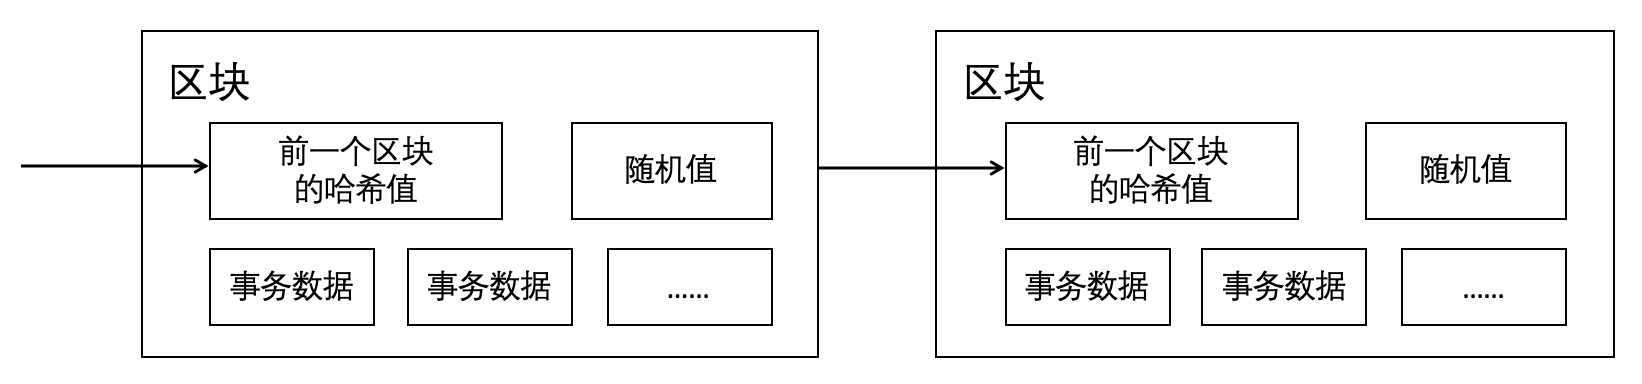
\includegraphics [width=400pt]{figures/hashchain.png}
\caption{区块链数据结构}
\label{fig:hashchain}
\end{figure}

正是由于上述重要特性,哈希算法被广泛应用于消息认证码、随机数产生、错误校正与检测等领域,而在区块链系统中,哈希算法主要用于检查数据是否被篡改,提供工作量证明,构造存在性证明这几个用途。区块链账本数据根据时间顺序组织成了若干个区块,一定时间内新发生的事务数据存储在一个新区块里,每一个区块都包含了上一个区块的哈希值,具体组织结构如图\ref{fig:hashchain}所示。

这一结构可以保障,如果区块链中任意区块里的数据被篡改,那么该区块的哈希值与后一区块记录的哈希值不相等。因此,区块链上的任何历史数据改动都能被检测。节点只需要存储最新区块的哈希值,即可通过计算检验历史上所有区块中的数据是否被篡改。

\begin{figure}
  \centering%
  \subcaptionbox{默克尔树数据结构\label{fig:merkle-tree}}
    {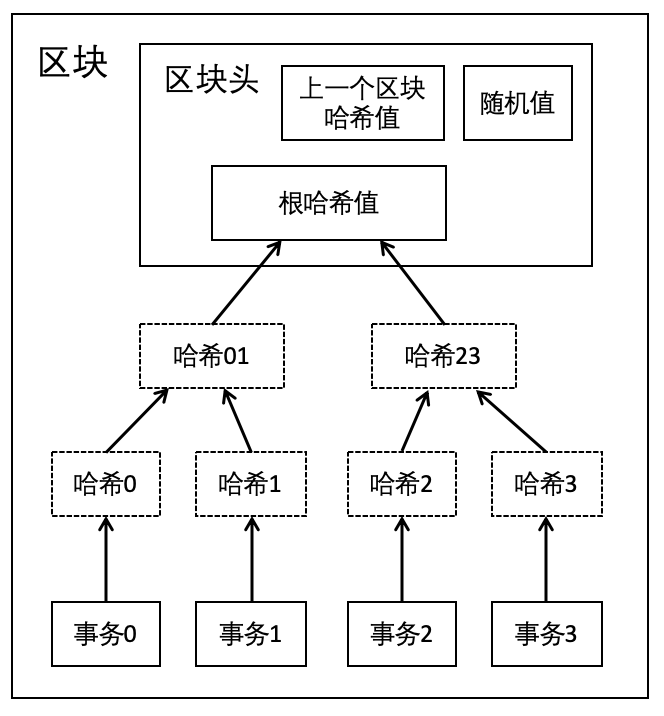
\includegraphics[width=150pt]{figures/merkle-tree.png}}%
  \hspace{2em}%
  \subcaptionbox{存在性证明\label{fig:merkle-proof}}
      {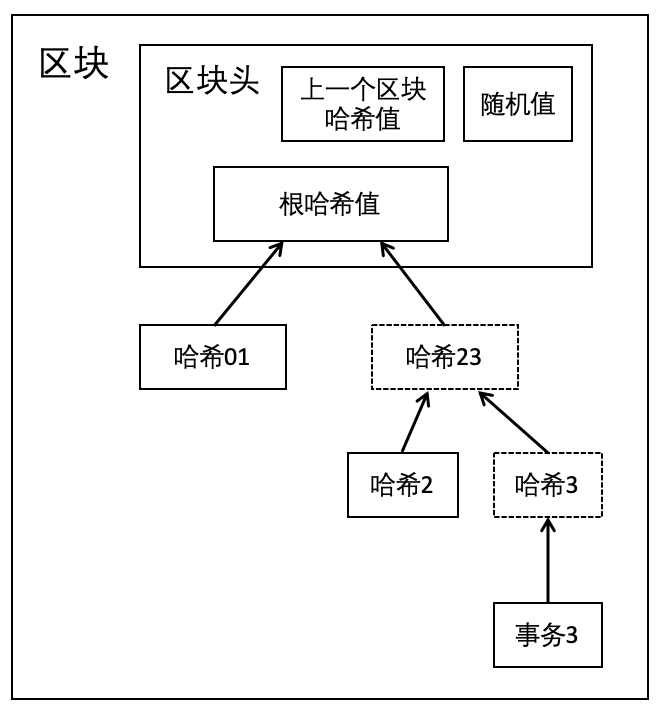
\includegraphics[width=150pt]{figures/merkle-proof.png}}
  \caption{默克尔树数据结构及存在性证明}
  \label{fig:merkle}
\end{figure}

而在每个区块中,哈希函数用于构建默克尔树,即哈希二叉树。如图\ref{fig:merkle-tree}所示,所有事务的哈希值通过二叉树结构进行哈希计算,最终计算得到根哈希值。该数据结构保证,任意事务数据的修改,都会影响到根哈希值。因此区块头中只需要存储根哈希值,就可以验证该区块中所有事务是否被篡改。

当用户需要通过根哈希值验证某事务是否在某区块中时,不需要验证该区块中所有事务数据,只需要由存储所有数据的节点提供该事务到根哈希值的路径上所有相关数据。如图\ref{fig:merkle-proof}所示,当用户希望验证事务3是否存储在区块中,只需要验证“事务3”,“哈希2”,“哈希01”这几个数据是否能通过哈希函数得到根哈希值。由哈希函数的抗碰撞性可以保证,证明节点不能提供虚假数据计算出同样的根哈希值。

\subsection{非对称密码体制和数字签名}

密码体制主要分为对称密码体制和非对称密码体制。简单来说,对称密码体制指加密算法中使用的加密密钥和解密算法中使用的解密密钥是相同的密钥,或者解密密钥能通过加密密钥计算得到。而非对称密码体制中,这两者不同,并且解密密钥不能通过加密密钥计算得到。

\begin{figure}[H]
\centering	
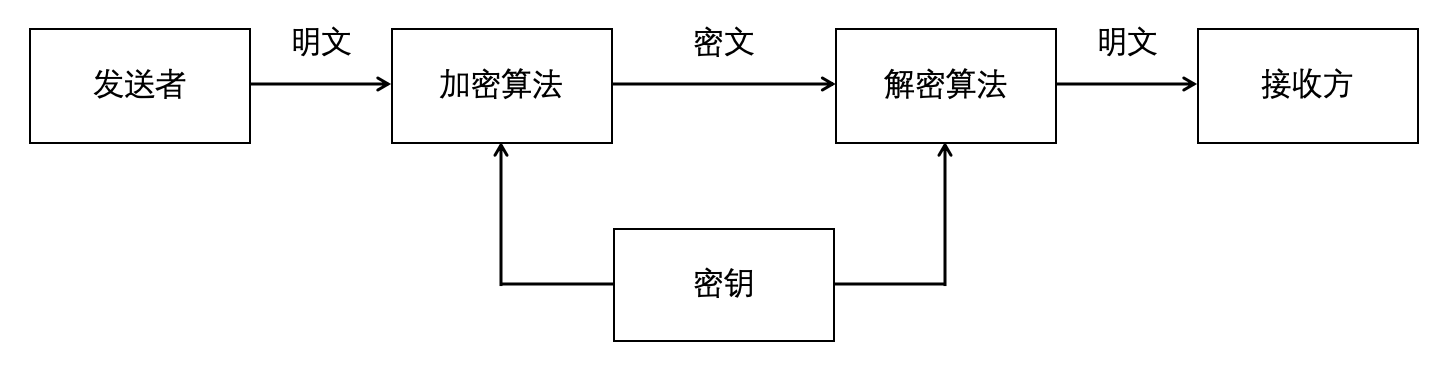
\includegraphics [width=400pt,height=100pt]{figures/sym-crypto.png}
\caption{对称密码体制的基本模型}
\label{fig:sym-crypto}
\end{figure}

如图\ref{fig:sym-crypto}所示,对称密码体制中,发送者先使用密钥和加密算法将明文加密为密文,然后传输密文给接收方,接收方使用解密算法和相同的密钥将密文解密回原始的明文。因为加密和解密算法使用的密钥需要相同,消息发送方和接收方必须在密文传输前通过安全信道进行密钥传输。因此对称密码体制面临密钥分配问题,目前主要通过通信双方直接进行密钥传输或者密钥分配中心进行密钥分发进行。然而实际的传输信道安全性并不理想,密钥在传输过程中被暴露的风险很大,增加了系统的脆弱性。另一方面,在有多个用户的网络中,任何两个用户之间都需要共享加密密钥。当网络中用户$n$很大时,需要管理的密钥数目为$C_n^2$,复杂度近似O($n^2$)。当有一个新用户加入时,需要产生$n$个秘密的密钥,并秘密分发给$n$个用户。

\begin{figure}[H]
\centering	
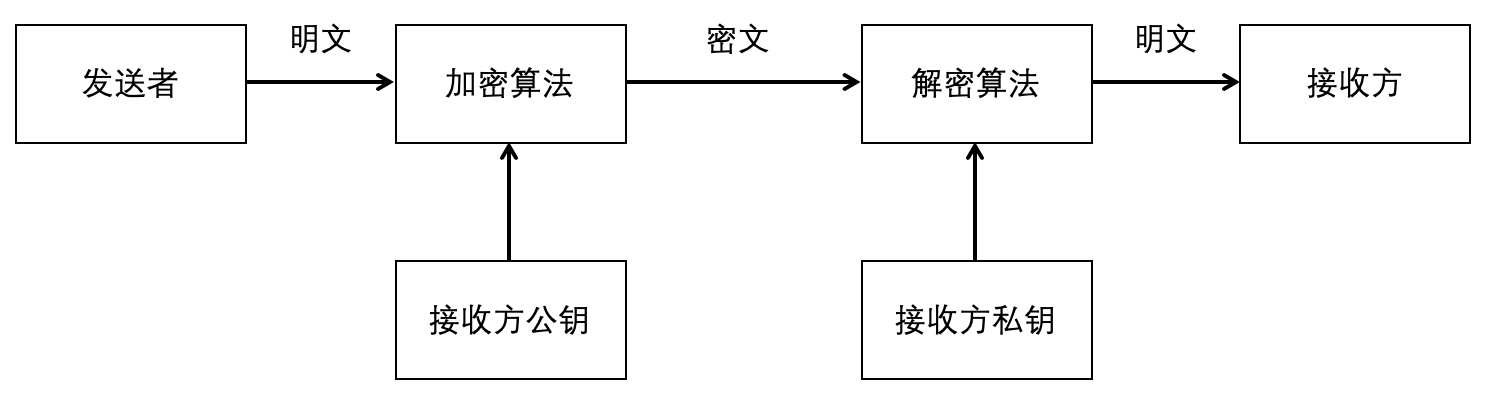
\includegraphics [width=400pt,height=115pt]{figures/asym-crypto.png}
\caption{非对称密码体制的基本模型}
\label{fig:asym-crypto}
\end{figure}

1976年,W.Diffie和M.Hellman在IEEE Trans.on Information刊物上发表了“ New Direction in Cryptography”文章,提出了“非对称密码体制“的概念,开创了密码学研究的新方向。如图\ref{fig:asym-crypto}所示,非对称密码体制中,密钥分为成对的加密密钥和解密密钥,其中加密密钥公开,解密密钥保密。公开的密钥可以作为用户的个人身份,由公开的加密密钥无法推导相应的解密密钥。因此即使将加密密钥公开也不会暴露解密密钥,不会损害密码的安全。因此,通信双方可以通过不安全的信道交换公钥,然后用对方的公钥对消息进行加密并传输,达到在不安全的信道上保密传输的效果。解决了对称密码体制中需要安全信道的问题,同时在密钥管理上也极大降低了网络中需要管理的密钥数量,从对称密码体制的$C_n^2$降低到$n$。对称密码体制与非对称密码体制在密钥分发、密钥管理等方面的区别主要如表\ref{tab:sym-asym}所示。

\begin{table}[htb]
  \centering
  \begin{minipage}[t]{1\linewidth}
  \caption{对称密码体制与非对称密码体制的区别}
  \label{tab:sym-asym}
    \begin{tabularx}{\linewidth}{lXX}
      \toprule[1.5pt]
      {\heiti 功能} & {\heiti 对称密码体制} & {\heiti 非对称密码体制} \\\midrule[1pt]
		密钥分发  & 需要事先进行安全的密钥分发 & 不需要事先进行安全的密钥分发,公钥可以在不安全的信道上传输 \\
		密钥管理  & 每个用户需要保存n个不同密钥用于与其他n个用户通信。当有新用户加入时,每个用户都需要和新用户共享一个新密钥,整个系统中需要存储O($n^2$)个密钥 & 每个用户只需要存储自己的公钥和私钥,整个系统中只需要存储O(n)个密钥 \\
		数字签名  & 不支持数字签名功能 & 支持数字签名功能 \\  
		性能  & 加密算法和解密算法简单,加解密速度较快 & 加密算法和解密算法需要进行复杂的数学运算,速度较慢 \\  
		安全性  & 安全性来源于混淆和置换 & 安全性通常基于数学难问题,部分假设未证明 \\ 
      \bottomrule[1.5pt]
    \end{tabularx}
  \end{minipage}
\end{table}

数字签名技术,通常也称为电子签名,指通过算法对数字消息进行处理得出签名。计算得到的数字签名同样具有手写签名的两大特性:可验证性和防伪造性。具体来说,数字签名具备以下特性:

\begin{enumerate}
 \item 任何人可以验证数字签名是否由消息的发送方生成。
 \item 任何人不能伪造发送方的数字签名,这也意味着发送方不能抵赖自己生成的数字签名。
 \item 任何人可以验证数字签名是否匹配发送的消息,因此可以验证消息从发送到接受过程中是否被篡改。对整个消息生成数字签名过于复杂,因此通常先对消息计算哈希值,然后生成哈希值的数字签名用于验证。
\end{enumerate}

在区块链领域,每个用户都可以通过特定算法独立生成任意多账户,即公私钥对。当用户发起事务时,需要用私钥生成事务数据的数字签名。当该事务涉及其他用户时,使用特定用户公钥生成的地址。

\section{共识协议}

多个节点为了达成关于某些数据的一致性,需要共同运行的共识协议进行保障。在传统的分布式领域,所有节点由同一公司或者组织运行,因此各节点的安全性、可信性都能得到保障,主要考虑节点出现共识模块关闭、消息网络延迟、节点宕机等异常情况。如果攻击者入侵控制系统中某些节点,则可以通过故意构造错误数据,以及对系统中不同节点发送不同的信息破坏共识过程。这类被入侵节点通常称为拜占庭节点,能抵抗部分拜占庭节点的共识协议称为拜占庭容错共识协议。

传统的分布式共识协议都是基于可信身份的投票机制,各节点知道当前共识系统中的节点数量以及各节点公钥,可以验证信息来源。而在区块链领域中,节点不受中心化组织管理,可以自由加入和退出。攻击者可以构建任意多的身份参与投票,因此在公有链领域需要采用无身份背书的共识协议,目前主要采用工作量证明共识协议。

\subsection{传统分布式共识协议}
\label{subsec:traditional-consensus}

传统分布式共识协议主要根据能否抵抗拜占庭节点,分为拜占庭容错共识协议和非拜占庭容错共识协议两类。本节主要介绍非拜占庭容错共识协议Paxos和Raft,以及拜占庭容错共识协议PBFT。

Leslie Lamport于1989年首次发布Paxos共识协议,Paxos协议通过处理器在协议中的角色来描述处理器的动作:客户端、接受者、提议者、学习者和领导者。在具体实现中,单个节点可能同时扮演一个或多个角色。

\begin{description}
  \item \textbf{[客户端]} 客户端向分布式系统发出请求,并等待响应。例如,对分布式文件服务器中的文件的读/写请求。
  \item \textbf{[接收方(选民)]} 接受方充当协议的容错“存储器”,接收方集合称为Quorums。发送给接收方的任何消息必须发送到接收方全体集合。从接收方接收到的任何消息都将被忽略,除非从集合中的每个接收方接收到相同的消息。
  \item \textbf{[提案方]} 提案方主张客户端请求,试图说服接收方同意它,并充当协调者,在冲突发生时推动协议继续,保障共识的活性。
  \item \textbf{[学习方]} 学习方充当协议的备份节点。一旦接收方同意了客户端的请求,学习者就可以采取行动执行请求并向客户端发送响应。为了提高系统的可用性,可以添加额外的学习者。
  \item \textbf{[领导方]} 系统达成一致需要领导方的提案并且协同。许多节点可能同时认为自己是领导者,但协议只保证在最终选出一个领导方时才能继续。如果两个节点都认为它们是领导方,可能会通过不断提出相互冲突的更新来阻止协议。然而,在这种情况下,仍能保障系统安全性。
\end{description}

一轮成功的Paxos共识从分布式系统中某节点接收到客户端发起的请求开始,到系统对该请求达成一致性结果结束。主要分为提议和接受两个阶段,每个阶段各包含两个步骤。

\begin{description}
  \item \textbf{[提议阶段]} 提议阶段包含准备和承诺两个阶段
  \begin{enumerate}
    \item 准备:收到客户端请求的节点充当提案方创建一个消息,我们称之为“准备”,它的编号为数字$n$。$n$不是要提议的值,它只是由提案方(发送给接收方)唯一标识这个初始消息的数字。编号$n$必须大于此提案方在先前的任何“准备”消息中所使用的编号。然后,它将包含$n$的“准备”消息发送给接收方集合。“准备”消息只包含数字n,不包含客户端发送的请求信息。
    \item 承诺:任何接收方都在等待来自任何提案方的“准备”消息。如果接收方收到一条“准备”消息,接收方检查编号$n$。如果$n$大于此前从任意提案方接受的所有提案编号,接受方必须返回一个“承诺”消息给提案方,并且忽略此后接收到的所有编号小于$n$的“准备”消息。如果接收方此前已接受某提案,则需要将包含接受的提案编号$m$和对应的值$w$的“提案”消息返回给提案方。
否则,如果n小于或等于接收方此前从任何提案方收到的提案编号,接收方可以忽略所收到的提案。
  \end{enumerate}

  \item \textbf{[接受阶段]} 提议阶段包含准备和承诺两个阶段
  \begin{enumerate}
    \item 接受请求:如果提案方收到来自大多数接收方集合的“承诺”消息,则需要为其“提案”消息设置一个值$v$,通常这个值表示从客户端接收到的请求数据。如果任何接收方曾经接受过提议,在提议阶段的承诺步骤中,会将接受的“提案”消息返回给提案方。提案方从接收到的所有“提案”消息中找出最大编号的提案,假设该提案的值为$z$,则需要将“提案”消息的值设为$z$。如果没有一个接收方返回“提案”消息,那么提案方可以选择自己的提案值$x$。提案者在选定值后,向接收方集合发送一个“接受”消息,包含编号$n$和提案值$v$,其中编号$n$与此前的“准备”消息一致。
    \item 接受:当接受者从提议者那里收到一条“接受”消息($n,v$),如果该节点已在提议阶段的承诺步骤中发出承诺只考虑编号大于$n$的提案时,则拒绝该消息。如果接收方尚未承诺,则该节点记录“接受”消息中的值$v$作为接受值。并将“接受”消息发送到提案方和每一个学习方。一个接受者可以接受多个提议,这可能发生在另一个提案方不知道正在决定的新值,并用更大的编号$m$开始新一轮。在这种情况下,接受者仍可以承诺并稍后接受新提议的值。这些提案可能导致接收方集合记录不同的值。然而,Paxos协议将保证接受方最终会同意某一相同的值。
  \end{enumerate}
\end{description}

2014年,Ongaro等人提出了Raft共识协议,简化Paxos协议的工作流程。相较于Paxos共识协议中各节点可以随时充当领导方发起提案,Raft协议首先通过领导选举推选出一个固定的节点担任领导方,当该节点故障时再做更换。在Raft协议中主要包含领导方,追随者和候选人三种角色。

\begin{description}
  \item \textbf{[领导方]} 领导方负责将记录备份给所有追随者,也需要不断发送心跳信息给追随者表明自己处于正常运行的状态。
  \item \textbf{[追随者]} 追随者负责接收并记录领导方发送的消息,同时通过心跳信息监听领导方的运行情况,一旦出现宕机等情况则转为候选人角色。
  \item \textbf{[候选人]} 当追随者发现领导方出现宕机等故障,将进入候选人角色,发起领导选举。
\end{description}

Raft协议的共识过程主要包含领导选举和记录备份两个部分,

\begin{description}
  \item \textbf{[领导选举]} 当系统开始运行Raft共识协议或者当现有的领导方出现故障时,所有参与节点需要选出一个新的领导方。系统共识的每一轮周期可能持续任意长的时间,都从领导选举开始。如果成功选出领导方,则本轮周期由该领导方负责后续的步骤,直到该领导方出现宕机等故障结束。如果选举失败,则开始新一轮周期,重新选举领导方。

  每轮领导选举由候选人发起。如果在周期$n$中,某节点在一段时间内没有收到领导者的心跳信息,那么该节点将成为候选人。它进入下一轮周期$n+1$,同时并向所有其他节点发送消息请求它们投票。当该节点收集到超过一半的投票,则成为新的领导方。如果在投票过程中,候选人节点接收到别的节点发出的消息,并且消息包含的周期值不低于$n+1$,则该节点停止选举并转为追随者。

  每个节点在每轮周期中只会进行一次投票,采用先到先得的方式。因此如果多个候选人同时请求投票,则可能所有候选人都收集不到超过一半的投票。在进入候选的时候,每个候选人会启动一个随机的定时器,定时器结束时进入下一轮周期,再次发起投票请求。

  \item \textbf{[记录备份]} 在选出领导后,领导方需要负责记录的备份。该领导方接受客户端发送的请求,每个请求包含一条指令。当请求作为一个新条目添加到领导方的日志之后,每个请求都作为“新增条目”消息转发给追随者。如果追随者出现宕机等情况不可用,领导方将不断地重新发送“新增条目”消息,直到日志条目最终被所有追随者存储。一旦领导方从大多数追随者收到条目已经被复制的确认,领导方会将该条目应用于本地的状态机,该请求处于“承诺”状态。同时也会提交领导方的日志中存在的所有条目。一旦追随者得知日志条目处于“承诺”状态,就将该条目应用到其本地状态机。
\end{description}

Paxos共识协议和Raft共识协议只能解决节点宕机和网络通信等故障异常,不能抵抗拜占庭节点的攻击。实用的拜占庭容错(PBFT,Practical Byzantine Fault Tolerance)共识协议于1999年提出,减少了此前拜占庭容错共识协议的时间和通信复杂度。PBFT共识协议主要包含“主节点”和“从节点”。PBFT协议的一次正常共识过程分为以下五个阶段:
 
\begin{figure}
\centering  
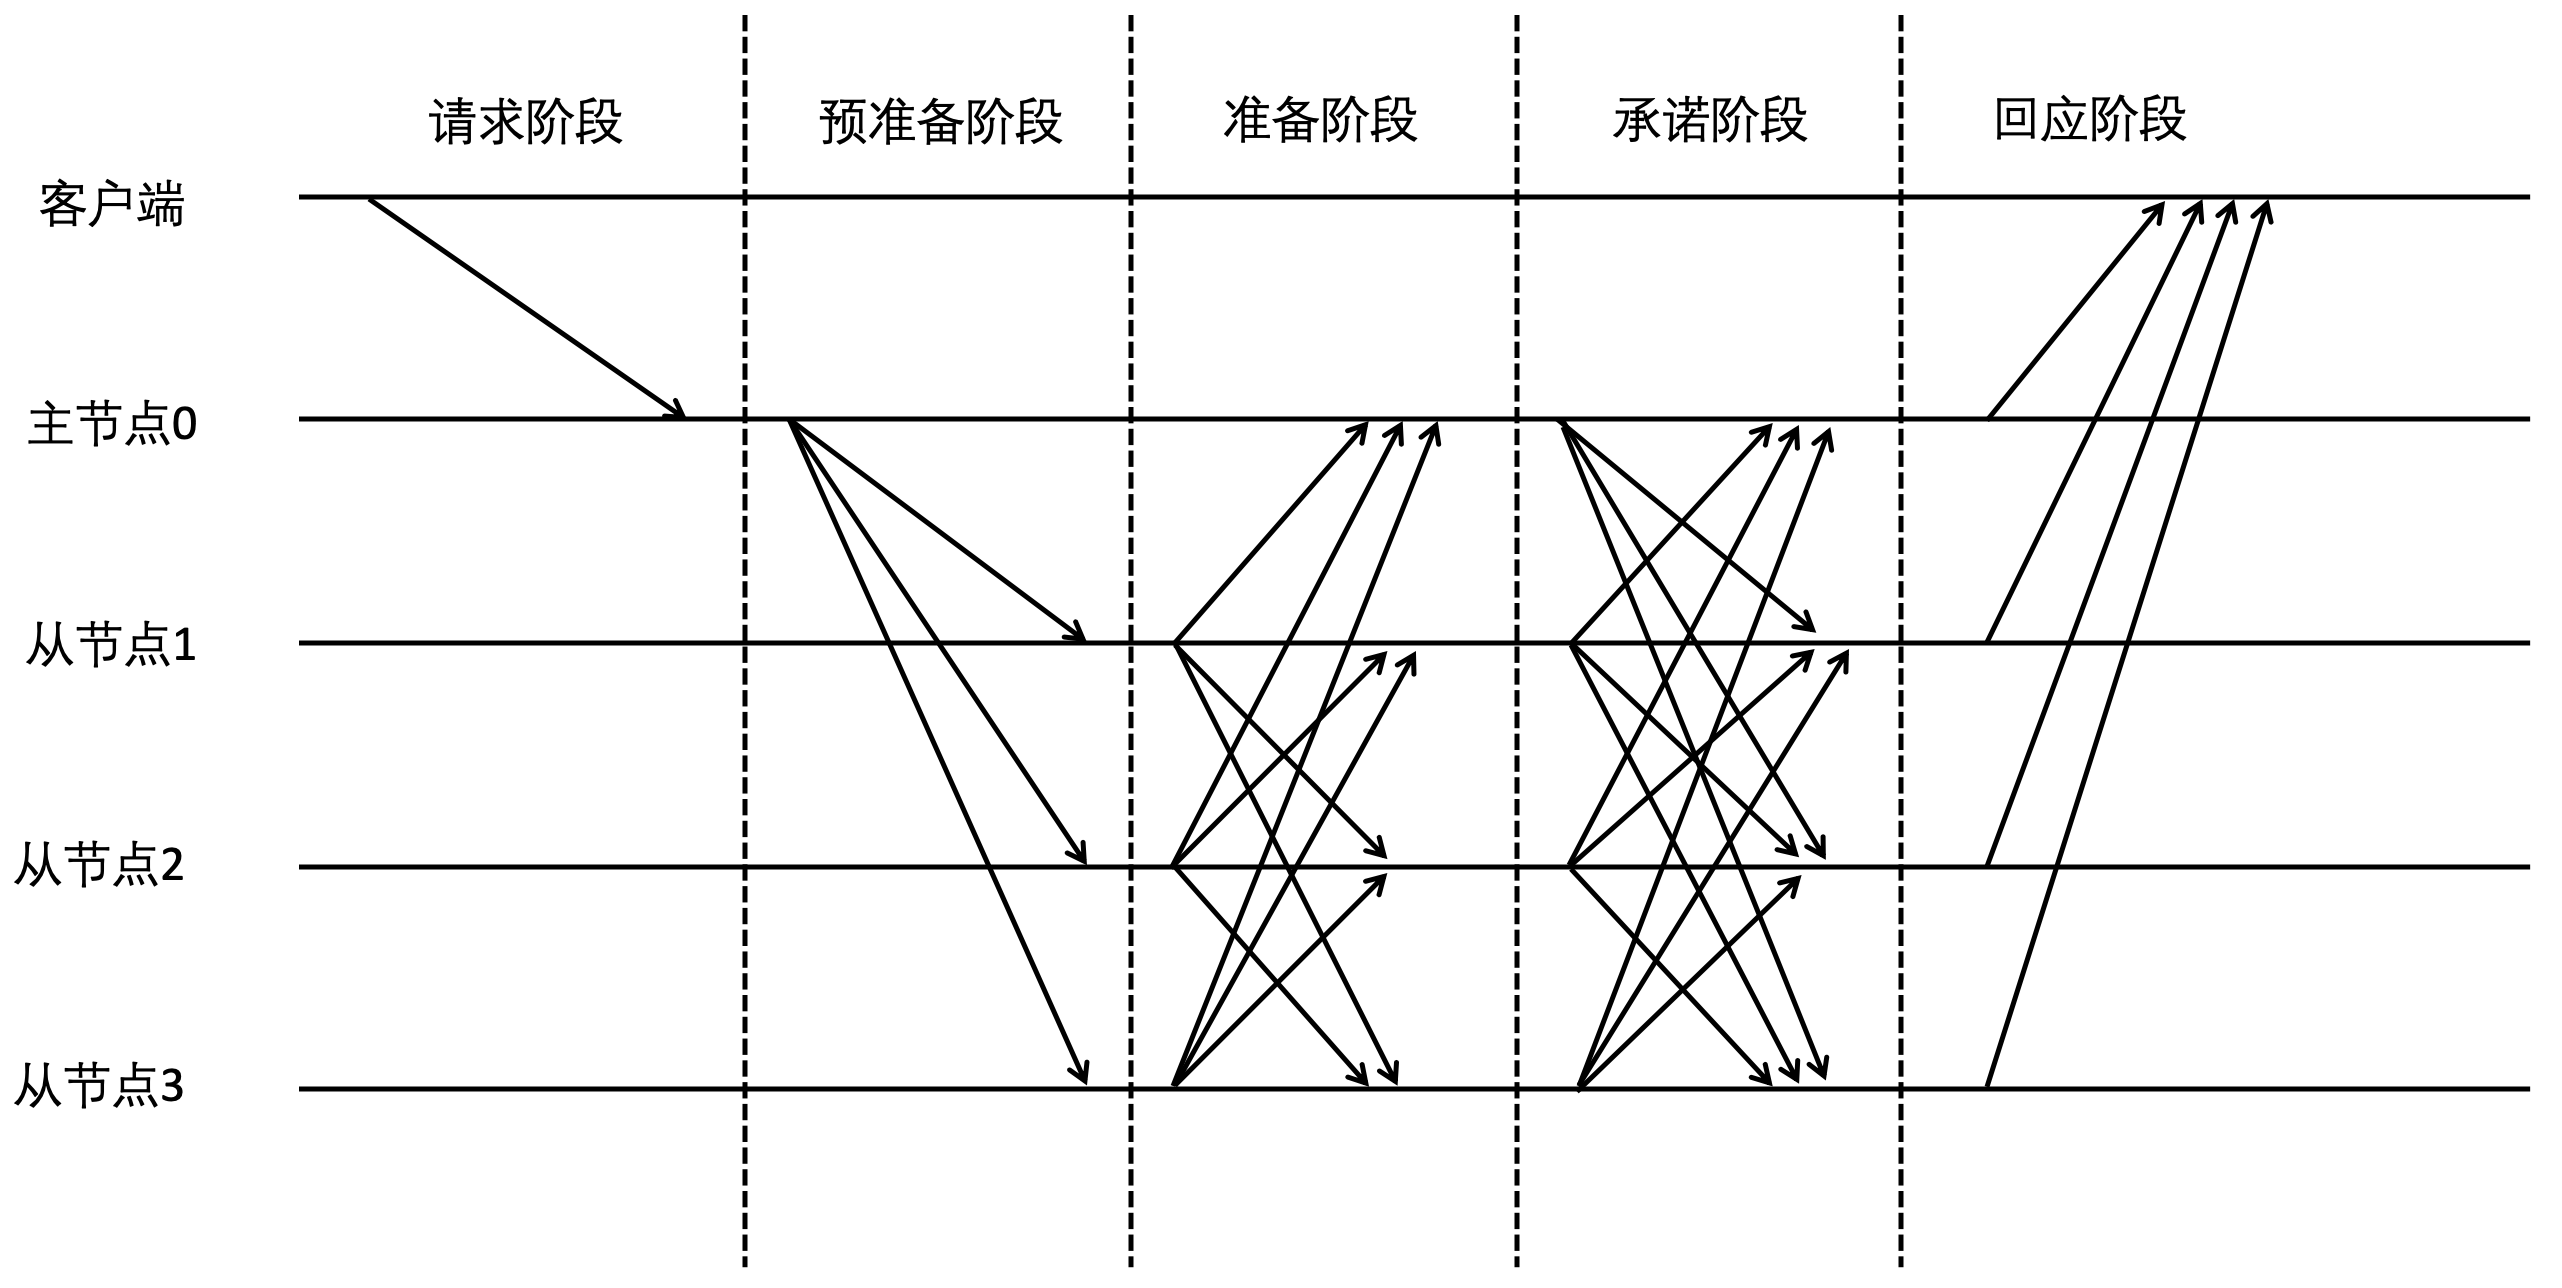
\includegraphics [width=400pt]{figures/pbft.png}
\caption{PBFT共识协议的正常流程}
\label{fig:pbft}
\end{figure}

\begin{enumerate}
  \item 客户端向系统中节点发送请求,接受到请求的节点将该请求转发给当前的主节点。
  \item 在预准备阶段,主节点将“预准备”消息广播给所有备份节点,包含请求的编号,请求内容等信息。
  \item 如果从节点接受“预准备”消息,则进入准备阶段。节点将“准备”消息广播给所有其他节点,包括主节点。
  \item 某节点一旦接收到不少于2f+1个“准备”消息,则进入“承诺”阶段,向其他节点广播“承诺”消息。
  \item 如果节点收到了相同请求的f+1个“承诺”消息,可以认为系统对该请求达成共识,将该请求记录到日志并作出对应的状态修改。客户端从接收到的所有回复中找出相同的大部分作为正确的回复。
\end{enumerate}

\subsection{工作量证明共识协议}
\label{subsec:work-proof}

在区块链领域,尤其在公有链网络中,节点可以自由加入或退出网络。需要采用无身份状态的共识协议。目前,公有链项目广泛使用比特币系统提出的工作量证明共识协议及类似协议。本节我们主要介绍比特币系统提出的工作量证明共识协议,以太坊项目改进的幽灵协议,以及Conflux项目进一步提出的Conflux共识协议。

工作量证明技术基于哈希函数的单向性、输出随机性和雪崩效应,要求用户通过修改消息后附带的$nonce$字段,达到整个消息哈希值在特定范围内。由于哈希函数的单向性,用户只能通过不断修改$nonce$值进行尝试。由哈希值每一位的独立随机性可以估计,该用户为了计算出合法的$nonce$值需要的计算工作量。而计算出合法的nonce值后,验证该输入是否合法只需要一次哈希计算。

比特币项目巧妙地将这一技术和第\ref{subsec:hash}节中提到的哈希链技术结合构建工作量共识协议。比特币系统中,打包新区块的节点需要在完成事务数据的组装后,不断修改nonce值,使得区块头的哈希值达到难度要求。当不同区块同时计算出合法的新区块时,网络中的节点并不能对选择哪一个区块达成共识,因此各节点可以选择任意区块并在之后进一步打包新区块,当某一分支积累的区块超过其他分支后,所有节点将放弃较短的分支,达成一致选择最长的分支。这也就是比特币系统的最长链法则。节点采用算力投票的方式达成共识,选择某一分支的节点算力之和越大,则该分支产生新区块的概率越高。

当达成一致后,除了最长链以外的分支区块都会被抛弃,这给了攻击者进行“双花攻击”的机会。攻击者通过分叉,将同一笔比特币先后发送给两个不同的账户,由于分叉的存在,在每个分支上交易都是合法的,这即是“双花攻击”。当攻击者拥有的算力超过正常节点的算力之和,即超过全网50\%的算力,攻击者可以创建分支超过正常节点维护的分支,这也就是“51\%算力攻击”。这一安全阈值并不绝对,原因就在于正常节点之间存在分叉,在投票恢复一致的过程中,正常节点的算力会分配到各分支上,此时恶意节点超过最长链不需要超过50\%的算力。分支越多,攻击者需要的算力越少,系统安全性越低。

最长链原则共识的分叉问题制约了其性能。为了提升区块链系统的性能,必须减少新区块的时间间隔,或者增大区块大小,包含更多交易。这两者都会导致新区块在网络中传播的时间相较于计算出块的时间比减小,进而导致更容易出现分支并且更难达成一致,这将导致系统安全性降低。

为了解决性能瓶颈,以太坊项目提出了幽灵协议,该协议将最长链共识原则改为最大子树共识原则。幽灵协议从创世块出发,在每次遇到分叉时,不断选择权重最大的子树作为下一个区块,每个子树的权重由该子树包含的所有区块难度和决定。即使正常节点之间出现算力分叉,也在同一个子树下进行计算新区块,可以共同抵抗攻击者构造的新分支,保障了系统安全性。

以太坊提出的最大子树共识原则利用了分叉区块的计算工作量,用于抵抗分叉攻击,提升系统安全性。但最终的链上数据只采用了一条链上的数据,除此以外的数据都被抛弃。这样可以保障整个区块链数据的一致性,避免状态矛盾。为了进一步提升系统性能,conflux协议在此基础上进一步利用了分叉块中未冲突的交易。conflux共识协议增加对分叉区块中的交易进行验证的步骤,通过对整个树状结构进行时期的划分,然后将各时期中与主链不矛盾的交易都认为合法交易,提升系统性能。


% !TeX root = ../main.tex

\chapter{基于区块链技术的访问控制系统BACS}
\label{chap:bacs}

本章首先介绍了基于属性的访问控制模型中的各组成部分以及工作流程,然后介绍了第三方授权认证框架OAuth 2.0的构架和工作流程。在此基础上,本章提出基于区块链的访问控制系统BACS。主要介绍该系统的框架设计和协议流程,以及对安全性进行简要分析。

\section{基于属性的访问控制模型}

基于属性的访问控制ABAC模型主要包含准备阶段和执行阶段,其中准备阶段负责收集访问控制系统中需要的属性集合,以及分析属性之间的关系,构建访问控制策略集合。而执行阶段主要负责验证并回应访问请求,以及对访问控制策略的更新。本文主要研究执行阶段中的访问请求验证步骤,提出基于区块链技术的方案,其他部分采用已有技术。

\begin{figure}[H]
\centering
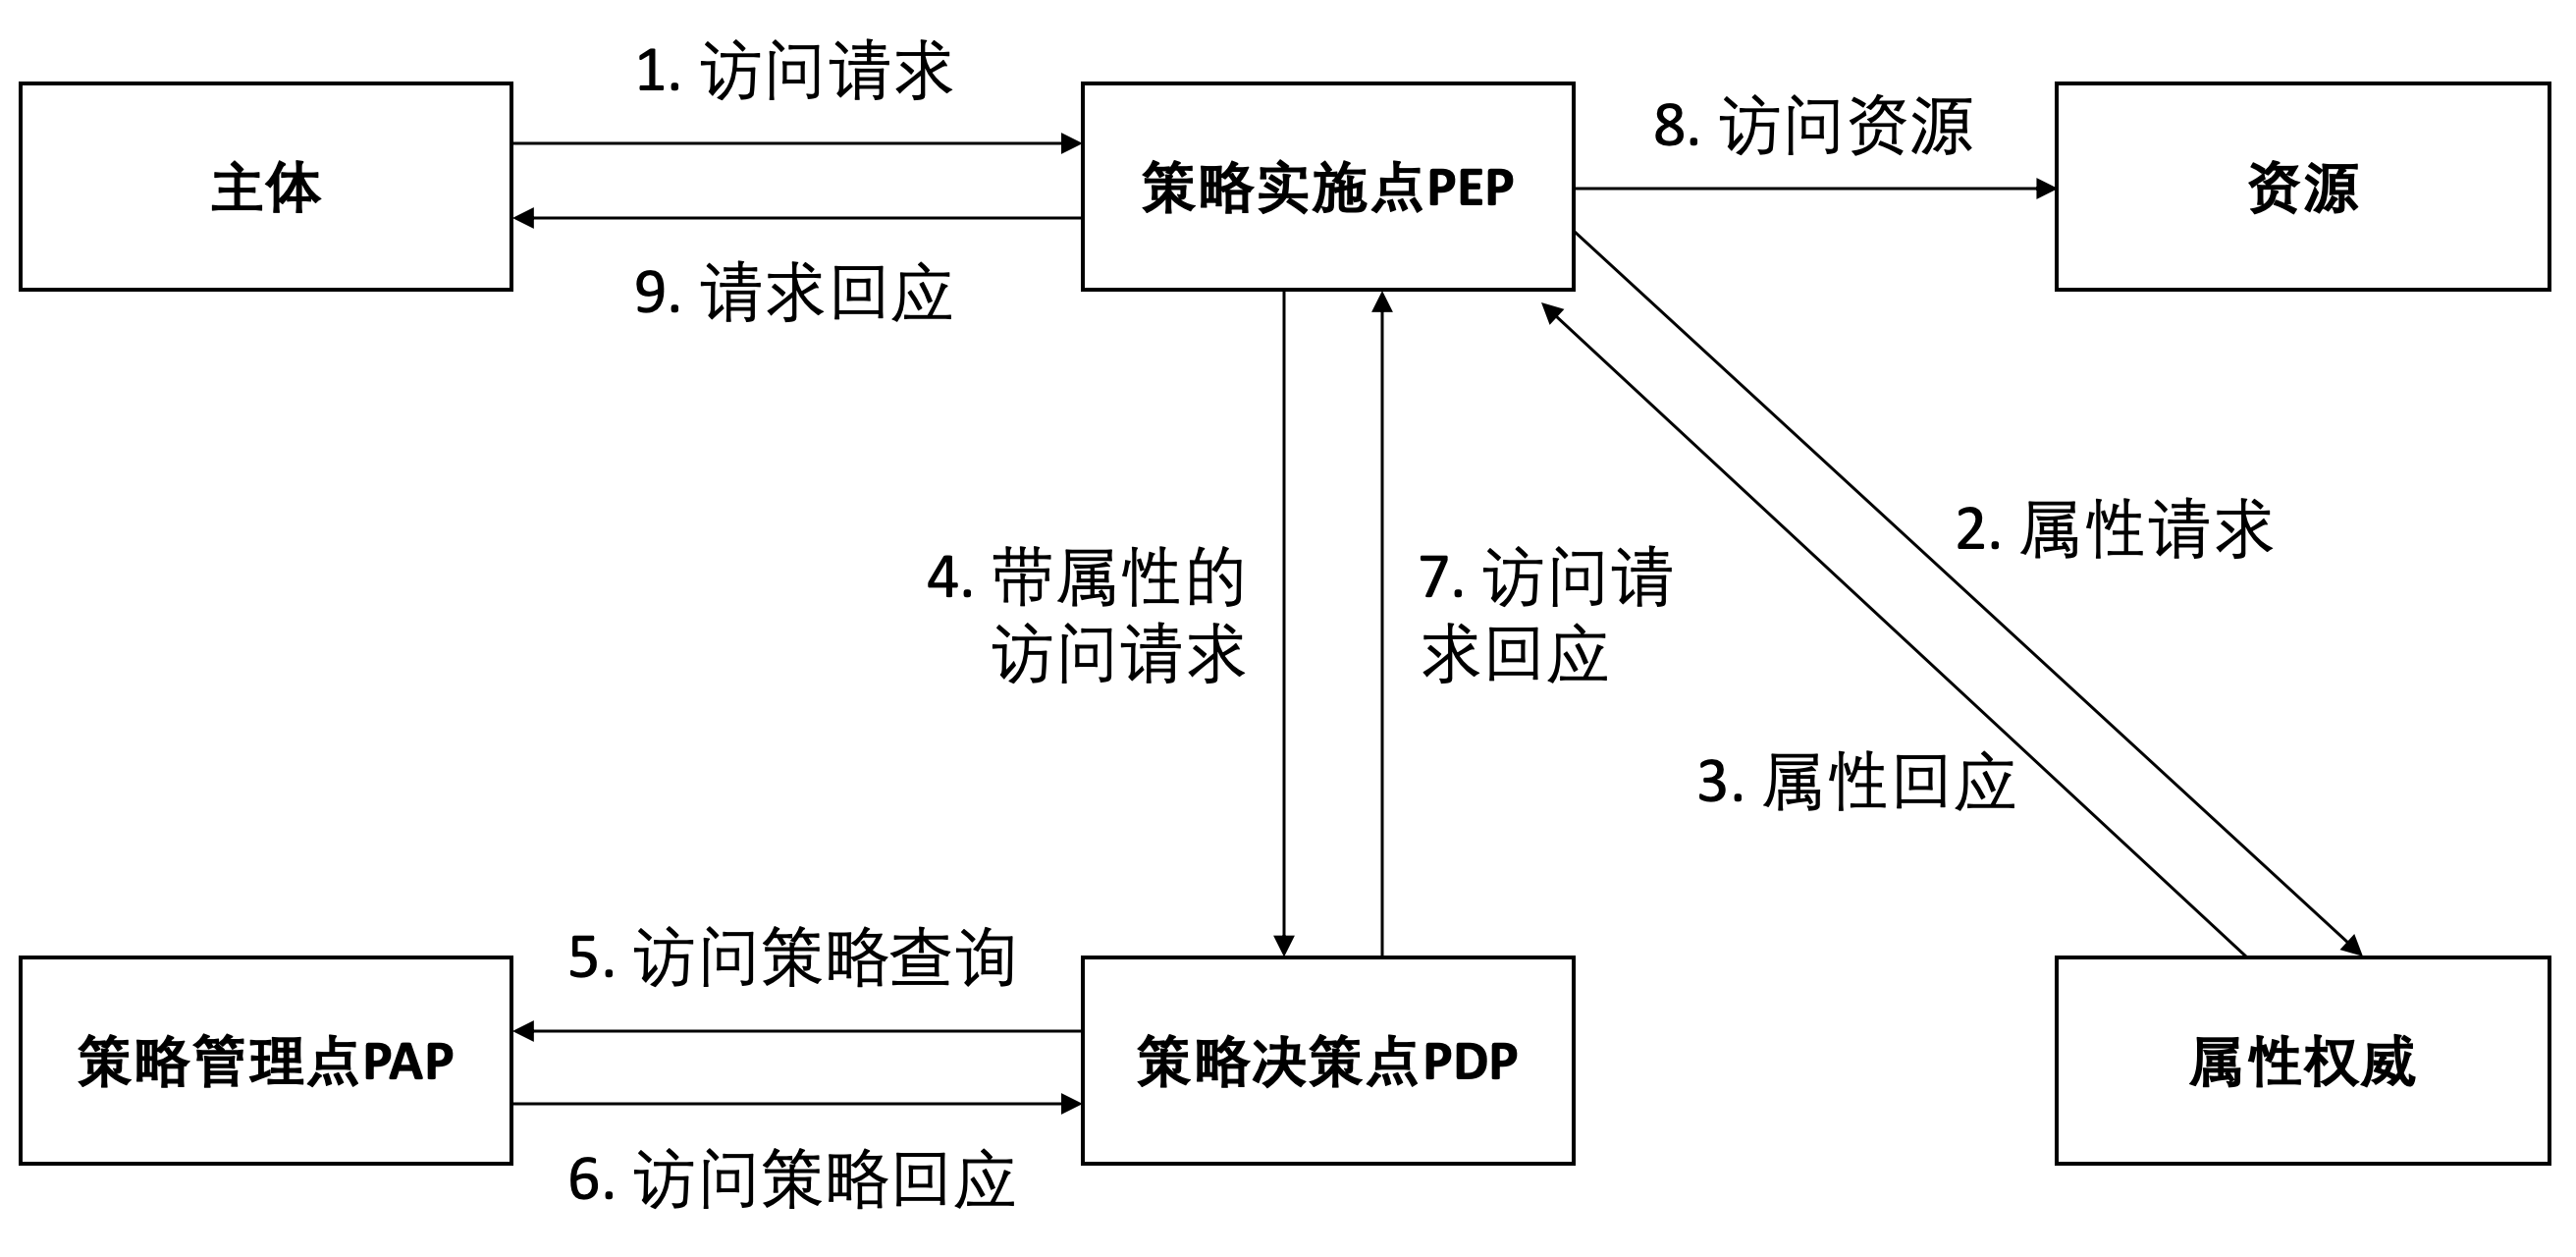
\includegraphics[width=12cm, keepaspectratio]{figures/abac.pdf}
\caption{基于属性的访问控制模型的执行阶段}
\label{fig:abac}
\end{figure}

如图\ref{fig:abac}所示,ABAC模型的访问请求验证主要包含主体,资源,策略实施点(Policy Enforcement Point,PEP),策略决策点( Policy Decision Point,PDP),策略管理点(Policy Administration Point,PAP),属性权威(Attribute Authority)。其中主体表示请求访问资源的用户,策略管理点管理策略列表,包含一系列属性的对应权限逻辑。属性权威返回对于该次请求的主体属性,资源属性,操作属性和环境属性。策略决策点根据请求,从属性权威获取相应的属性值,然后根据策略管理点返回的特定属性策略决策该请求是否通过,策略实施点根据该决策执行相应操作,完成对资源的操作。

\section{第三方授权认证框架}

在互联网时代,网络中各平台分别管理用户的不同数据,为了提升易用性,方便第三方应用访问用户数据,OAuth 2.0框架被各大平台广泛应用。该框架中,主要有客户端,资源所有者,资源服务器和授权服务器四种角色,其中资源所有者将数据存储在资源服务器,给第三方客户端进行授权,客户端通过授权服务器换取凭证,用于访问资源服务器的数据。

\begin{figure}
\centering  
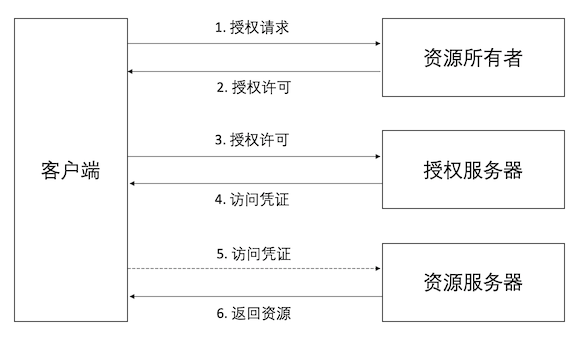
\includegraphics [width=11cm]{figures/oauth.pdf}
\caption{OAuth 2.0框架中授权码模式的正常工作流程}
\label{fig:oauth}
\end{figure}

这里主要介绍OAuth 2.0框架中授权码模式的正常工作流程。如图\ref{fig:oauth}所示,该流程主要有以下3个阶段:

\begin{enumerate}
  \item 客户端向资源所有者发送授权请求,请求获取相应的资源访问权限。资源所有者收到请求后,检查请求的权限,通过验证后返回对应的授权许可给客户端。
  \item 客户端将授权许可发送给授权服务器,授权服务器验证后将对应资源的访问凭证返回给客户端。
  \item 客户端将访问凭证发送给资源服务器,资源服务器验证凭证后执行相应操作,并将结果返回给客户端。
\end{enumerate}

OAuth框架可以支持细粒度、动态和灵活的特权管理,适用于各种访问控制模型,在Google和Facebook等许多公司广泛使用。然而,整个授权认证过程依赖于中心化的授权服务器,存在内部和外部攻击的安全风险。

\section{访问控制系统BACS}

为了解决传统授权服务中存在中心化授权服务器的问题,本文提出基于区块链的访问控制系统BACS,采用联盟链代替中心化的授权服务器,存储管理授权数据记录,增强系统安全性和可信性。本节主要介绍该系统的框架设计,协议流程以及对安全性进行简要分析。

\subsection{第三方授权框架}

\begin{figure}
\centering
\includegraphics[width=14cm]{figures/framework.pdf}
\caption{第三方授权服务框架图}
\label{fig:framework}
\end{figure}

如图\ref{fig:framework}所示,BACS系统包含三类角色,“客户端”作为资源请求者,它请求资源所有者进行授权,并最终请求区块链节点访问资源。“资源所有者”在区块链节点上存储资源,在需要时授予“客户端”访问受保护资源的权限。BACS系统用“区块链节点”组成的联盟网络代替OAuth框架中的中心化认证服务器和资源服务器,每个节点具有平等的地位,由资源服务器和授权服务器组成。其中资源服务器存储用户不同的资源,授权服务器共同参与用户授权数据的存储和管理。

\begin{description}
  \item[\textbf{资源所有者}] 资源所有者存储自己的资源在资源服务器,并在需要时授予客户端访问受保护资源的权限。
  \item[\textbf{客户端}] 客户端指资源请求者,通过向资源所有者发送请求获取授权,并访问资源服务器获取资源。不同于OAuth框架中客户端需要提前注册,任何用户都可以独自创建账户作为客户端。
  \item[\textbf{区块链节点}] 联盟链网络由若干互联的区块链节点组成。每个节点包含授权服务器和资源服务器。其中资源服务器分别存储资源所有者的不同资源,并采用ABAC模型验证操作请求。所有节点的授权服务器共同运行共识协议,管理记录资源所有者对客户端的授权,并维护账户的属性状态。
\end{description}

\subsection{第三方授权服务工作流程}
\label{sec:protocols}
本节介绍BACS系统中授权服务的工作流程。整个协议主要分为5个步骤,分别对应于图\ref{fig:framework}中的工作流程。具体步骤如下:

\begin{enumerate}
  \item 客户端向资源所有者发送$Authorization Request$,其中主要包含客户端的地址和请求授权的属性。
  \item 资源所有者检查$Authorization Request$,如果同意则生成相应的$Authorization Grant$并且发送给任何区块链节点。
  \item 如果接收到的$Authorization Grant$有效,则区块链节点将接受并在网络中传播它。共识过程结束后,授权将被打包到一个新的区块中,并记录到区块链上。
  \item 获得授权后,客户端找到存储需要访问资源的区块链节点,并发送$Operation Request$给该节点的资源服务器。
  \item 资源服务器根据授权服务器提供区块链上账户的主体属性,存储的资源属性以及基于属性的访问控制策略来验证$Operation Request$,根据验证结果回应客户端。
\end{enumerate}

接下来将详细介绍各步骤的细节。首先介绍后续涉及的一些密码学表示,对于消息$m$,我们定义$H(m)$表示$m$的哈希值,并且用$\langle m \rangle_{\sigma_{i}}$ 表示消息 $m$ 以及节点$i$对 $H(m)$ 的签名。可以用于验证该消息的真实来源以及是否在传输中被篡改。

\subsubsection{区块链和属性状态}

该系统中,区块链是用来存储授权记录的基本数据结构,每个区块记录一系列授权信息,每个授权信息包括发送方地址,接收方地址,授权属性,授权有效期以及用于验证的签名等信息。为了在本系统中,我们采用了以太坊项目中的账户状态机制,而非比特币项目中的未花费输出UTXO(Unspent Transaction Output)机制,因为状态设计更适合ABAC模型。我们将账户中的余额等信息修改为属性状态,区块链记录每个账户拥有的所有属性以及nonce值,每个属性包括属性名和有效期。

根据区块链上记录的信息,我们可以计算包含地址、nonce和属于地址的属性状态的每个帐户的状态。状态保存在内存中,可用于验证授权或操作。在区块链上添加新块时,全局状态将根据新块中的授权进行更改。我们可以将全局状态视为区块链的当前结果。对于帐户状态中的$nonce$值,每个帐户都有一个$nonce$值,其值为0。地址D的一次授权记录在区块链上时,地址D的一次授权将增加1。任何与nonce值不匹配的授权都将被拒绝,可以防止重播攻击。

\subsubsection{区块生成算法}

 \begin{algorithm}
 \floatname{algorithm}{Algorithm}{}
 \caption{Block Generation}\label{alg:blockGeneration}
   \begin{algorithmic}[!htbp]
   \renewcommand{\algorithmicrequire}{\textbf{Input:}}
   \renewcommand{\algorithmicensure}{\textbf{Output:}}
   \REQUIRE $AuthorizationPool, AUTH\_LIMIT, PreviousBlock$
   \ENSURE  $Verification$
    \STATE $auths \gets ChooseAuths(AuthorizationPool, AUTH\_LIMIT)$
    \STATE $prevHash \gets H(PreviousBlock)$
    \STATE $timestamps \gets CurrentTime()$
    \STATE $newBlock \gets NewBlock(prevHash, auths, timestamps)$
   \RETURN $newBlock$
   \end{algorithmic}
 \end{algorithm}

联盟网络中的节点会将一段时间内接受到的授权信息打包到一个新区块中,在比特币系统中这个时间间隔是10分钟,而在以太坊中是15秒,动态调整的具体方法在前文章节中有所介绍。而在本系统中,为了保障访问控制系统的延迟可接受,我们设置区块间隔为2秒,区块生成的具体算法在算法\ref{alg:blockGeneration}中介绍。

\subsection{改进的PBFT共识协议}
\label{subsec:adapted-pbft}

在前文第\ref{subsec:traditional-consensus}节中,我们介绍了多种共识协议。我们在访问控制系统中采用了改进的PBFT协议。区块链网络广播中的节点向其他节点发送请求。经过一段时间后,主节点将合法请求打包成块。然后将该块广播到网络中,与其他节点达成共识。

主节点、备份节点和视图更改基本采用PBFT协议的设计。但针对区块链技术需求进行以下改进,PBFT协议中的主节点在接收到来自客户端的请求时开始协商过程。BACS系统中,主节点每2秒启动一次协商,并将最多1000个授权打包到一个新区块中。当备份节点发现主节点似乎发生故障或被攻击时,将发生视图更改,这与PBFT协议中的视图变化相同。除此之外,当一段时间后,系统中的节点也会自动进行视图更改。这可以防止来自恶意主节点的黑名单攻击。在区块链系统中,生成新块的节点可以选择其中包含的事务以及先后顺序,恶意节点可以拒绝打包黑名单中帐户的事务。因此,不断的视图更改可以防止来自恶意主节点的黑名单攻击。改进的PBFT共识协议中设计了各类消息的数据结构,如图\ref{fig:pbft-data}所示。接下来介绍各阶段的具体实现算法。

\begin{figure}
  \centering%
  \subcaptionbox{“预准备消息”数据结构\label{fig:pre-prepare}}
    {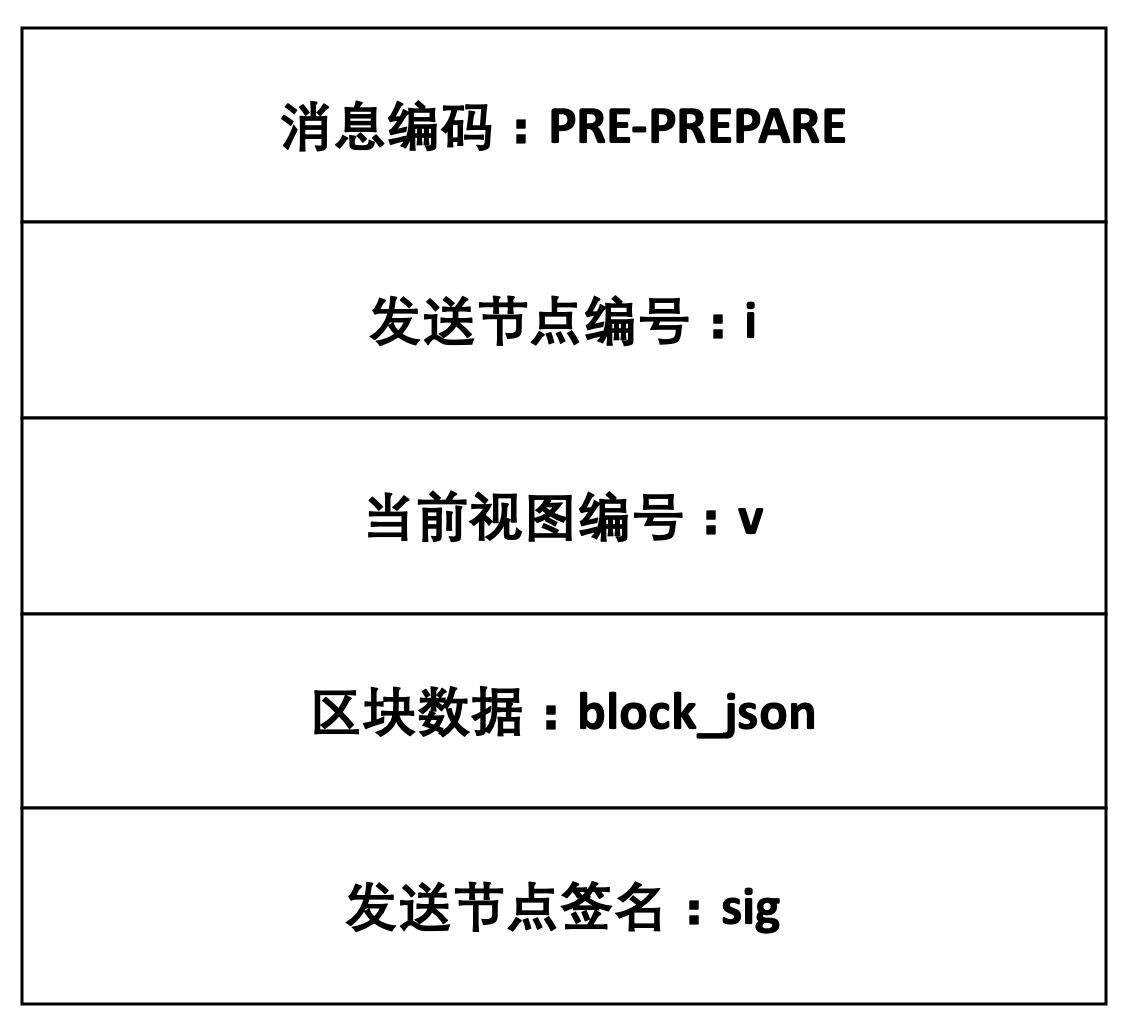
\includegraphics[width=6cm]{figures/pre-prepare.pdf}}%
  \hspace{2em}%
  \subcaptionbox{“准备消息”数据结构\label{fig:prepare}}
      {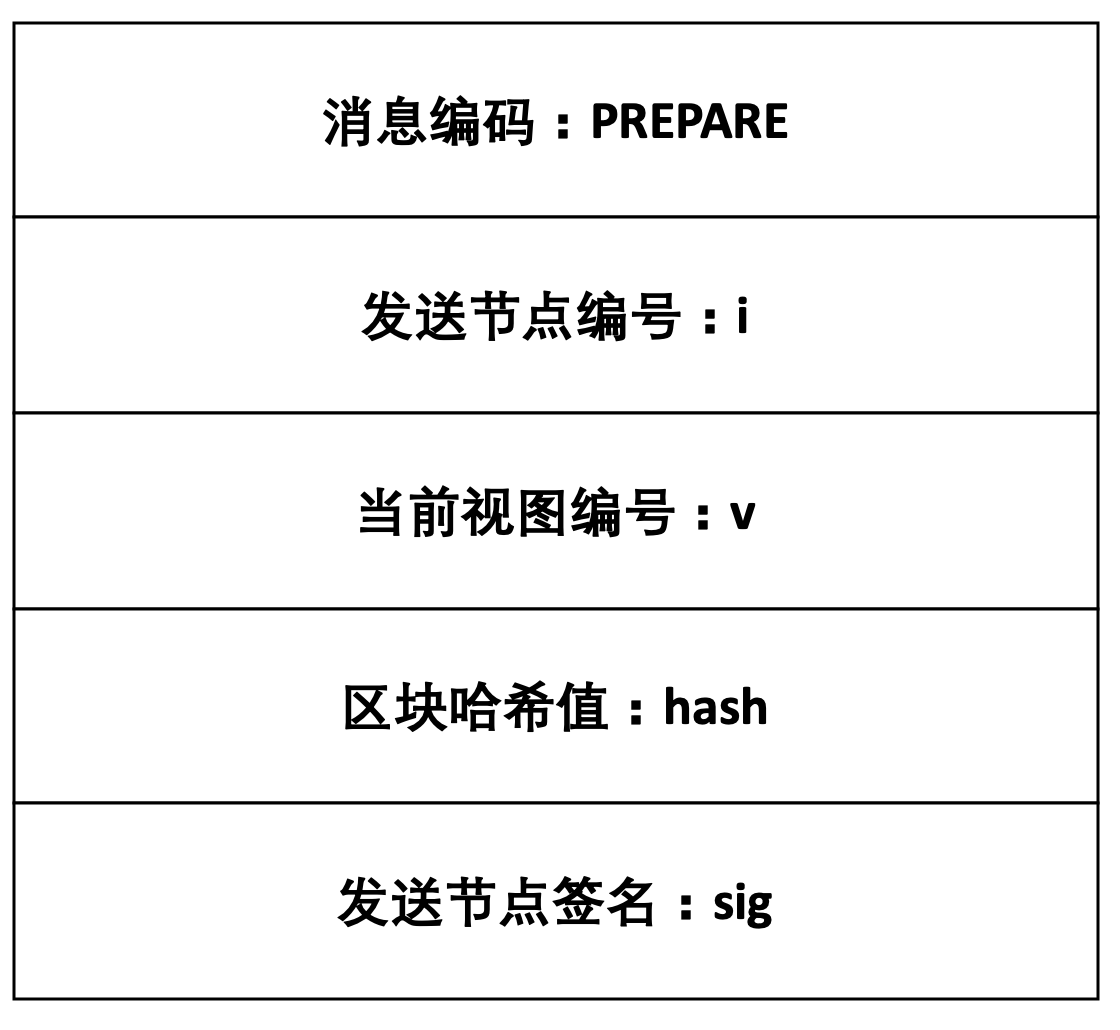
\includegraphics[width=6cm]{figures/prepare.pdf}}

  \subcaptionbox{“承诺消息”数据结构\label{fig:commit}}
      {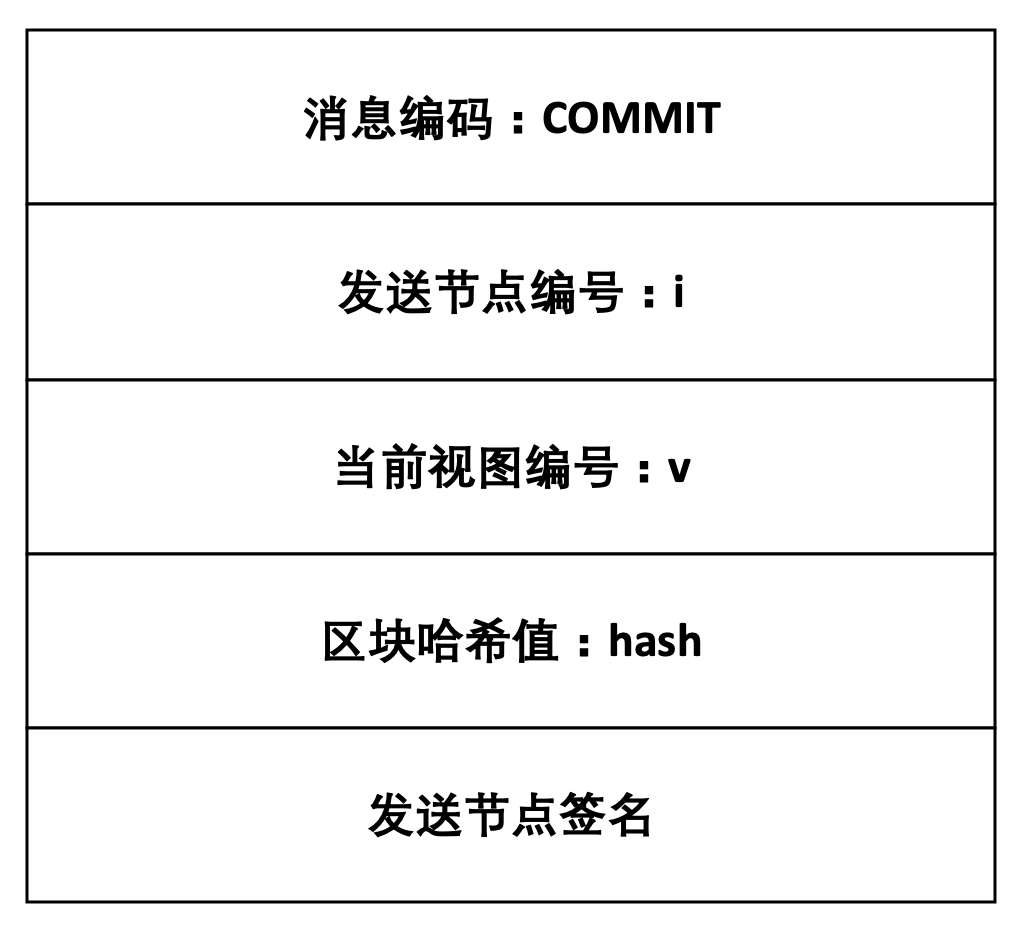
\includegraphics[width=6cm]{figures/commit.pdf}}
  \hspace{2em}%
  \subcaptionbox{“视图更新消息”数据结构\label{fig:viewchange}}
      {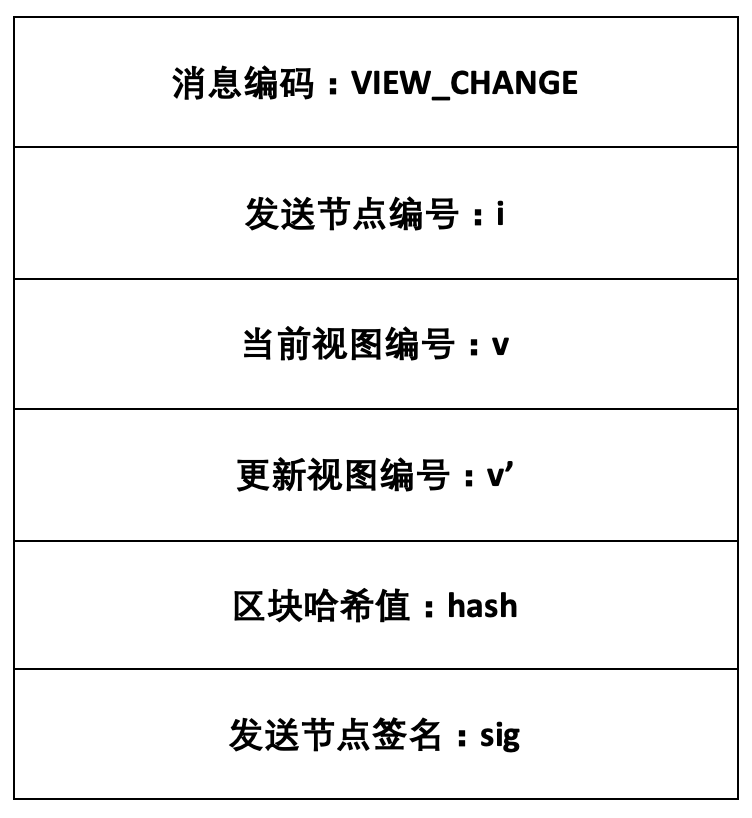
\includegraphics[width=6cm]{figures/viewchange.pdf}}
  \caption{共识协议中各类消息的数据结构}
  \label{fig:pbft-data}
\end{figure}

\subsubsection{预准备阶段}

 \begin{algorithm}
 \floatname{algorithm}{Algorithm}
 \caption{生成预准备信息}\label{alg:preprepareGen}
   \begin{algorithmic}[H]
   \renewcommand{\algorithmicrequire}{\textbf{Input:}}
   \renewcommand{\algorithmicensure}{\textbf{Output:}}
   \REQUIRE $blockchain, authorizationPool, AUTH\_LIMIT,$ $sk, viewID$
   \ENSURE  $pre$-$prepare$
    \STATE $prevBlock \gets blockchain.LastBlock()$
    \STATE $block$ $\gets$ $BlockGenration(prevBlock, AUTH\_LIMIT,$ $authorizationPool)$
    \STATE $pre$-$prepare \gets NewRequest(viewID, block)$
    \STATE $signature \gets sk.Sign(request)$
    \STATE $pre$-$prepare.Signature \gets signature$
   \RETURN $pre$-$prepare$
   \end{algorithmic}
 \end{algorithm}

当一个新区块过程开始,所有节点进入预准备阶段。这一阶段中,主节点从授权池中选择一系列合法的授权,并且打包到一个新区块中。然后,主节点广播预准备信息$\langle PRE$-$PREPARE, v, i, block \rangle_{\sigma_{i}}$ 给所有备份节点,其中 $v$ 表示当前的视图编号,$i$ 表示主节点的节点编号。具体预准备信息$pre$-$prepare$的创建如算法\ref{alg:preprepareGen}所示。

 \begin{algorithm}[H]
 \floatname{algorithm}{Algorithm}
 \caption{验证预准备信息}
   \begin{algorithmic}[H]\label{alg:prepreVerify}
   \renewcommand{\algorithmicrequire}{\textbf{Input:}}
   \renewcommand{\algorithmicensure}{\textbf{Output:}}
   \REQUIRE $pre$-$prepare$, $N$, $ViewID$, $i$, $PkList$
   \ENSURE  $Verification$
    \STATE $viewID$, $nodeID$, $timestamps$, $signature \gets Parse(pre$-$prepare)$
    \IF {$viewID \ne ViewID$}
      \RETURN $false$
    \ENDIF

    \IF {$nodeID \ne ViewID \% N$}
      \RETURN $false$
    \ENDIF

    \STATE $hash \gets H(pre$-$prepare)$
    \IF {$CheckSignature(PkList[i], hash, signature) \ne true$}
      \RETURN $false$
    \ENDIF
   \RETURN $true$
   \end{algorithmic}
 \end{algorithm}

当备份节点接受到主节点发送的预准备信息$pre$-$prepare$后,验证过程如算法\ref{alg:prepreVerify}所示。如果通过验证,备份节点将接受该信息并进入准备阶段。否则,该节点可以认为主节点被恶意控制或者宕机,将会发起视图切换,请求选举出下一个正常节点作为新的主节点。

\subsubsection{准备阶段}

 \begin{algorithm}
 \floatname{algorithm}{Algorithm}
 \caption{生成准备信息}
   \begin{algorithmic}[H]\label{alg:prepareGen}
   \renewcommand{\algorithmicrequire}{\textbf{Input:}}
   \renewcommand{\algorithmicensure}{\textbf{Output:}}
   \REQUIRE $pre$-$prepare, nodeID, sk, NeighborList$
   \ENSURE  $prepare$

    \STATE $blockHash$ $\gets$ $H(pre$-$prepare.Block)$

    \STATE $viewID \gets pre$-$prepare.ViewID$
    \STATE $prepare \gets NewPrepare(viewID, nodeID, blockHash)$
    \STATE $signature \gets sk.Sign(prepare)$
    \STATE $prepare.Signature \gets signature$
   \RETURN $prepare$
   \end{algorithmic}
 \end{algorithm}

如果备份节点 $i$ 接受了预准备信息$pre$-$prepare$,该节点进入准备阶段。节点$i$生成准备信息$\langle PRE$-$PARE, v, i, blockHash\rangle_{\sigma_{i}}$,其中视图编号$v$和预准备信息中的视图编号一致,$i$ 表示该备份节点的节点编号,$blockHash$ 表示预准备信息$pre$-$prepare$中包含区块的哈希值。具体细节在算法\ref{alg:prepareGen}中介绍。然后该备份节点将生成的准备信息 $prepare$广播给其他所有节点,包括主节点在内。一旦某个节点从不同的来源节点(包括自己)接收到$2f+1$个拥有相同$v$和 $blockHash$的准备信息,该节点将会进入承诺阶段。

\subsubsection{承诺阶段}

进入承诺阶段的节点获知网络中大部分正常节点(至少f+1个)已经接受该信息。节点$i$将生成并广播承诺信息$\langle COMMIT, v, i, blockHash \rangle_{\sigma_{i}}$ 给所有节点,表明该节点将接受这一新区块作为共识结果。承诺的生成过程如算法\ref{alg:commitGen}所示。

 \begin{algorithm}
 \floatname{algorithm}{Algorithm}
 \caption{Commit Generation}
   \begin{algorithmic}[H]\label{alg:commitGen}
   \renewcommand{\algorithmicrequire}{\textbf{Input:}}
   \renewcommand{\algorithmicensure}{\textbf{Output:}}
   \REQUIRE $prepare, nodeID, blockHash, sk$
   \ENSURE  $commit$

    \STATE $viewID \gets prepare.ViewID$
    \STATE $blockHash \gets prepare.blockHash$
    \STATE $commit \gets NewCommit(viewID, nodeID, blockHash)$
    \STATE $signature \gets sk.Sign(prepare)$
    \STATE $commit.Signature \gets signature$
   \RETURN $commit$
   \end{algorithmic}
 \end{algorithm}

当某个节点从不同来源节点接收到 $2f+1$个合法的承诺信息,该节点可以确认该新区块至少被$f+1$个正常节点接受,因为在接收的$2f+1$个承诺信息中,至多只有$f$个来源于拜占庭节点。然后该节点可以将该区块记录在区块链上,并更新账户状态。

\subsection{安全分析}

我们假设了一个敌手模型,将所提出的原型与OAuth 2.0框架进行比较。我们考虑存在一个非常强大的敌手可以入侵授权服务器,控制所有存在安全隐患的节点,监听信道并针对授权数据进行重播攻击。但是,我们假设敌手不能违反上面提到的密码学技术的安全性。例如,敌手不能计算出两个不同的消息,都拥有相同哈希值,也不能计算出特定公钥对应的私钥或在不知道私钥的情况下伪造特定私钥的签名。在考虑这一敌手模型假设的情况下,该系统比OAuth 2.0框架具有以下两个方面的优点:

\begin{enumerate}
  \item 敌手可以监听并重放授权数据。在OAuth 2.0框架中,授权将在指定的时间之后过期,通常为10分钟。但是,在过期之前,它可能会导致重播攻击,敌手可以获取授权。而在我们的系统中,用户的授权数据一旦记录到区块链,用户的计数器将增加1,因此该授权或操作将无效,授权服务器将不再接受它。在这个场景中,我们的系统比OAuth 2.0框架更安全。

  \item 攻击者可以入侵授权服务器。在OAuth 2.0框架中,所有第三方应用程序的所有应用账号和密码都存储在授权服务器中,因此敌手可以获取这些信息,伪装成任何应用程序,甚至可以发出伪造的令牌来访问受保护的资源。由于授权服务器是集中式的,因此无法停止它。在我们的系统中,由于采用了具备拜占庭容错的PBFT共识协议,除非攻击者同时控制网络中的$(n-1)/3$个节点,否则攻击无法成功。
\end{enumerate}

上述安全分析表明,BACS系统通过非对称加密技术和引入区块链网络,有效增强第三方授权服务框架的安全性。
%!TeXroot=../main.tex

\chapter{区块链上隐私保护技术分析}
\label{chap:privacy}

在区块链系统的实际使用中,为了保证区块链上记录数据的可溯源、可验证等特性,所有数据都必须公开给区块链网络中的所有节点。这一特性在保障安全、可验证的同时,导致恶意攻击者可以直接获取区块链账本中记录的数据,并通过分析数据窥探用户隐私。攻击者通过分析区块链账本中记录的交易数据,发掘其中规律,将用户的不同地址、交易数据关联,并进一步对应到用户的现实身份[7-14]。这类分析攻击主要分为地址聚类和身份定位两阶段。地址聚类阶段根据用户行为特征将可能属于同一用户的地址、交易进行聚类,得到地址间关联关系。身份定位阶段搜集与区块链地址相关联的用户信息,例如论坛、交易所等服务记录的与链上地址对应的手机、邮箱、IP地址等用户链下信息,再根据搜集到的信息确定用户身份,关联该用户所有地址与交易信息,揭露该用户的所有历史记录。

近年来,许多研究者开始关注区块链系统中的隐私问题,该领域中相应的防御技术也不断出现。在区块链隐私分析上,祝烈煌等人从身份隐私和交易隐私两方面分析区块链中的隐私问题,身份隐私指用户身份信息和区块链地址之间的关联关系,交易隐私指区块链中存储的交易记录及背后的知识。Sarah等人提出用抗追溯性来度量区块链中用户信息的匿名性。本文从账本存储和网络通信两个方面,分析区块链系统中隐私信息可能泄露的内容和方式。从账本存储角度,需要保护用户存储在区块链账本上的数据记录所包含的隐私信息;从网络通信角度,需要保护区块链网络中的节点隐私及网络通信中的流量等隐私信息。在隐私保护技术方面,祝烈煌等人[30]从网络层、交易层和应用层出发分别描述区块链隐私保护面临的威胁以及采用的保护技术。Merve等人和李旭东等人将研究分为两大类:基于比特币系统的研究和针对比特币系统进行拓展和替换的研究。

本章对比特币系统以外的区块链隐私保护技术进行更大范围的技术介绍与对比。主要通过技术实现原理,将保护技术划分为地址混淆,信息隐藏和通道隔离,并对各类技术抽象出通用模型,然后介绍各类隐私保护技术的实现及对比。其中地址混淆机制通过交易交换不同用户的资产,对同一用户不同地址间的关联关系进行混淆,从而破坏地址聚类的假设前提;信息隐藏机制通过零知识证明、同态加密等密码学技术加密区块链账本中记录的隐私信息,同时保持账本正确性的可验证;通道隔离机制在区块链网络中设置访问权限,将需要权限访问的数据保护在特定通道中。

\section{区块链隐私及威胁}

传统的区块链系统中通常采用假名机制和广播机制保护用户隐私。其中假名机制指用户可以独立生成任意数量的区块链地址,不需要通过注册或者认证机制。同一用户生成的不同地址可以单独使用,彼此间不存在任何关联关系。因此,仅通过区块链地址无法关联到用户的真实身份,该机制能隔离用户在区块链上不同操作的记录。广播机制指区块链系统通过p2p网络传输数据,网络中采用洪水广播协议传播消息,接受节点无法判断消息来源是消息的直接发起者还是转发者,从而保护消息真实发起者的身份。

假名机制和广播机制能在一定程度上保护区块链用户的隐私安全。但在实际应用中,用户隐私仍面临各类威胁,主要存在于记录数据的分布式账本和区块链去中心化网络中各节点的相关信息。为了保证去中心化系统的正确性和安全性,区块链系统中的所有节点共同维护一致的分布式账本,记录区块链系统中的所有历史数据,用于验证用户提交的新事务的合法性。为了所有节点都能验证账本的正确性,账本中所有数据保持公开,因此账本数据能被攻击者轻易获取,攻击者通过分析公开账本中的记录严重威胁用户隐私。此外,区块链系统采用去中心化网路进行通信,在非许可链系统中,节点加入网络不需要任何身份认证,这在增强了扩展性的同时也导致攻击者可以自由部署节点加入网络,监听网络中各节点隐私信息以及网络中通信信息。本章围绕这两部分介绍需要保护的隐私内容及对应的威胁方式。

\subsection{账本隐私及威胁}

区块链账本记录了区块链系统中的各类事务数据,由于目前区块链系统主要应用于密码货币领域,因此区块链账本主要记录交易数据。交易模型主要分为未花费交易输出(UTXO,UnspentTransactionOutput)模型和账户(Account)模型两类[34]。部分攻击方式针对特定的交易模型,例如交易网络构造攻击和资产追踪攻击针对UTXO模型。账本隐私主要包含以下内容:
交易内容隐私:账本记录的单笔交易内容,包含交易发起方、交易接受方、交易金额以及附带数据等隐私信息。
账户地址隐私:区块链地址与交易的关联关系,包含账户地址的交易记录、账户余额以及不同账户地址间交易关联等隐私信息。
用户身份隐私:用户和区块链地址、交易的关联关系,包含同一用户的交易记录、资金余额等隐私信息。
在区块链系统的实际应用中,用户常需要发起多输入交易,即存在多个输入资产的交易。该交易需要每个输入地址的签名,可以由一个或多个用户生成。由于多个用户对同一交易进行签名的过程较为复杂,通常多输入交易由同一用户生成。此外,在基于UTXO模型的交易系统中,未花费资产只能使用一次,因此当花费资产超过交易所需资产时,用户将超出部分的资产转移到自己的另一账户地址中。用于接受超出部分资产的账户地址通常称为找零地址。针对账本隐私包含的各类隐私,目前的主要攻击方式为账本分析攻击,通过分析区块链账本数据,利用用户常见的交易规律,构建账户地址与交易之间以及用户与账户地址之间的一对多对应关系,威胁账本地址隐私与用户身份隐私。攻击者根据区块链系统的设计与上述使用特征提出以下假设:

\begin{enumerate}
	\item 假设1 多输入交易的所有输入地址为同一用户所持有。
	\item 假设2 交易的找零地址和输入地址为同一用户所持有。
\end{enumerate}

2013年,Reid等人下载了比特币系统2009年1月3日至2011年7月12日的全部账本数据,通过分析数据首先构建交易网络。交易网络中节点表示单次交易,节点间的有向边为交易间的输出-输入对,表示前一次交易的输出作为后一次交易的输入,每条边同时记录了交易金额以及交易时间。部分交易网络如图\ref{fig:sub-network}所示。

\begin{figure}
\centering
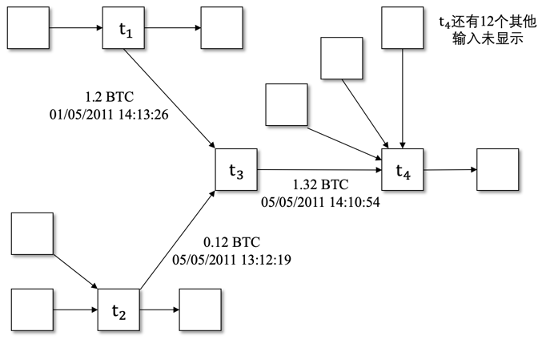
\includegraphics[height=7cm]{figures/sub-network.png}
\caption{交易网络示例}
\label{fig:sub-network}
\end{figure}

在交易网络的基础上,提取所有多输入交易,构建账户地址间的非完全网络。如图\ref{fig:nc-user-network}所示,非完全网络中节点表示地址,节点间有向边表示地址间交易的时间和金额。Reid等人根据中本聪提到的多输入交易关联风险提出假设1,即假设多输入交易的所有输入地址为同一用户所有。基于这一假设,在非完全网络的基础上,可以聚合属于同一用户的所有地址,进而构建用户网络,用户网络中节点表示一个用户,节点间的有向边表示用户间资产流动信息。

\begin{figure}[ht]
  \centering%
  \subcaptionbox{非完全网络中的局部示例\label{fig:nc-network}}
    {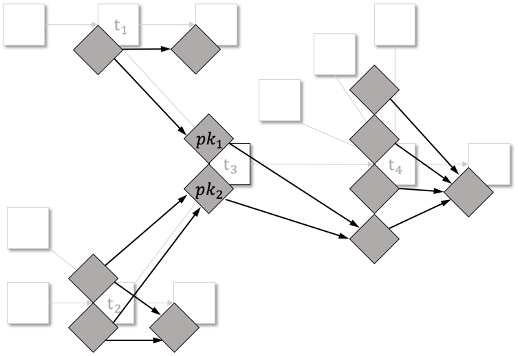
\includegraphics[height=7cm]{figures/nc-network.png}}%
  \hspace{4em}%
  \subcaptionbox{用户网络中的局部示例\label{fig:user-network}}
      {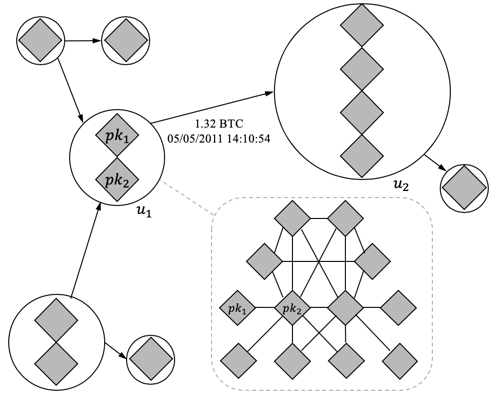
\includegraphics[height=7cm]{figures/user-network.png}}
  \caption{非完全网络与用户网络示例}
  \label{fig:nc-user-network}
\end{figure}

2013年,Androulaki等人[8]根据区块链钱包的应用特征提出了挖掘找零地址的方法,如果一个交易拥有两个输出,其中一个为已出现过的地址,另一个为新地址,则将新地址视为找零地址,并提出了假设2,即交易的找零地址和输入地址为同一用户所持有。为了验证假设的正确性,Androulaki等人在大学中构建了模拟的密码货币使用环境,通过搜集用户使用记录,并利用假设1和假设2进行分析,挖掘出40\%左右用户的真实身份。受此启发,Meiklejohn等人[9]给出了“找零地址”更完善的定义:
	
找零地址如果交易t中的一个输出公钥地址pk满足以下所有特征,则可将pk视为“找零地址”。

\begin{enumerate}
	\item $d_{addr}^{+}(pk) = 1$该地址pk在非完全网络中入度为1,即在区块链账本中首次出现。
	\item 交易t为铸币交易以外的普通交易。铸币交易即生成新区块时发布奖励的交易。
	\item 不存在$pk^{'}\in  output(t)$且$pk^{'}\in  input(t)$,即不存在“自找零地址”。
	\item 不存在$pk^{'}\in  output(t)$,$pk^{'} \neq pk$且$d_{addr}^{+}(pk^{'}) = 1$,即pk为输出地址中唯一首次出现的地址。
\end{enumerate}

综上所述,账本隐私内容主要集中于单次交易的内容及隐藏在多个相关交易之后的用户身份、账户余额等隐私信息。这部分信息记录在公开的区块链账本中,攻击者可以通过分析账本挖掘出其中的关联信息,威胁用户的账本隐私。

\subsection{网络隐私及威胁}

区块链系统通过去中心化的P2P网络进行节点间通信,而在非许可链系统中的网络不存在准入限制,这在增强了扩展性的同时也带来了潜在的风险。攻击者可以任意部署节点,监听网络中各节点隐私信息以及网络通信信息,甚至尝试对正常节点发起攻击。区块链网络主要存在以下隐私内容:

\begin{description}
  \item[\textbf{节点隐私}] 节点自身的隐私内容,包含节点网络IP、软件版本、服务器系统等隐私信息。
  \item[\textbf{通信隐私}] 节点间通信隐私内容,包含节点间通信的数据内容以及通信流量情况。
\end{description}

2013年,Reid等人尝试利用BitcoinFaucet公开的区块链地址及IP地址对应关系进行分析,揭露比特币用户与实际物理位置的对应关系,该尝试只涉及到很少的节点。Bitnodes网站通过部署大量节点,探测全球范围内的比特币节点信息,其中IP地址分布信息如图\ref{fig:bitcoin-dis}所示(截图于2019年08月01日)。

\begin{figure}
\centering
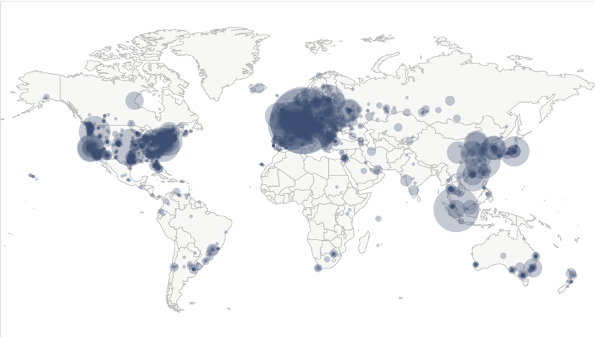
\includegraphics[height=7cm]{figures/bitcoin-dis.png}
\caption{世界范围内比特币节点分布情况}
\label{fig:bitcoin-dis}
\end{figure}

探测攻击严重威胁节点隐私,更进一步,攻击者通过大量探测可以将区块链中广播的数据与实际发起节点关联,尽管区块链网络采用洪水广播的方式保护实际发起人,但是在布置大量探测节点后,攻击者有很大概率找出消息的真实发起节点。2011年,Kaminsky在黑帽大会上提出假设,假设第一次接受到消息时的来源节点即为该消息的真实发起节点。

\begin{figure}[ht]
  \centering%
  \subcaptionbox{模式1 单一转发者\label{fig:trans-pattern1}}
    {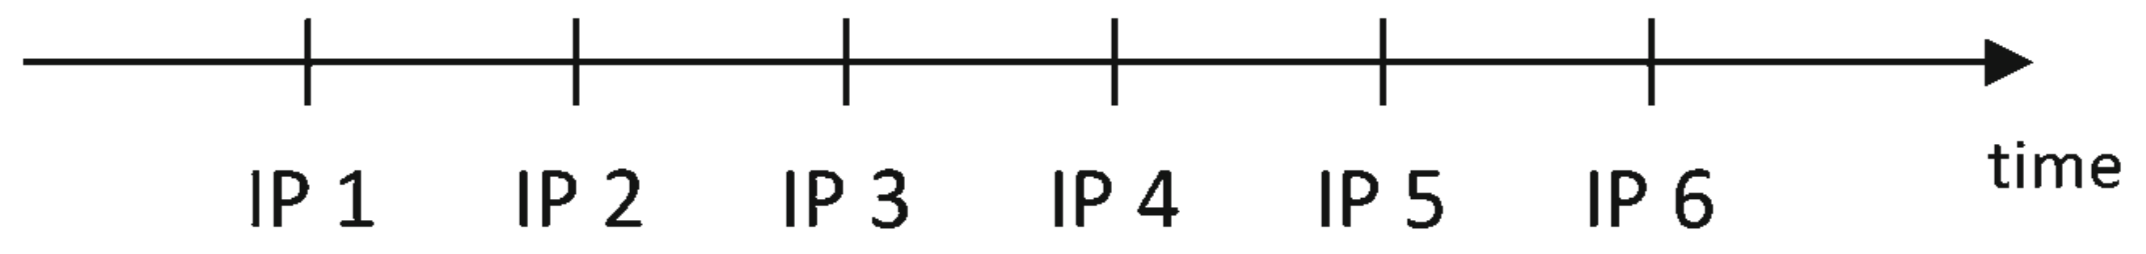
\includegraphics[width=7cm]{figures/trans-pattern1.png}}%
  \hspace{2em}%
  \subcaptionbox{模式2 多转发者,无重复转发者\label{fig:trans-pattern2}}
  	{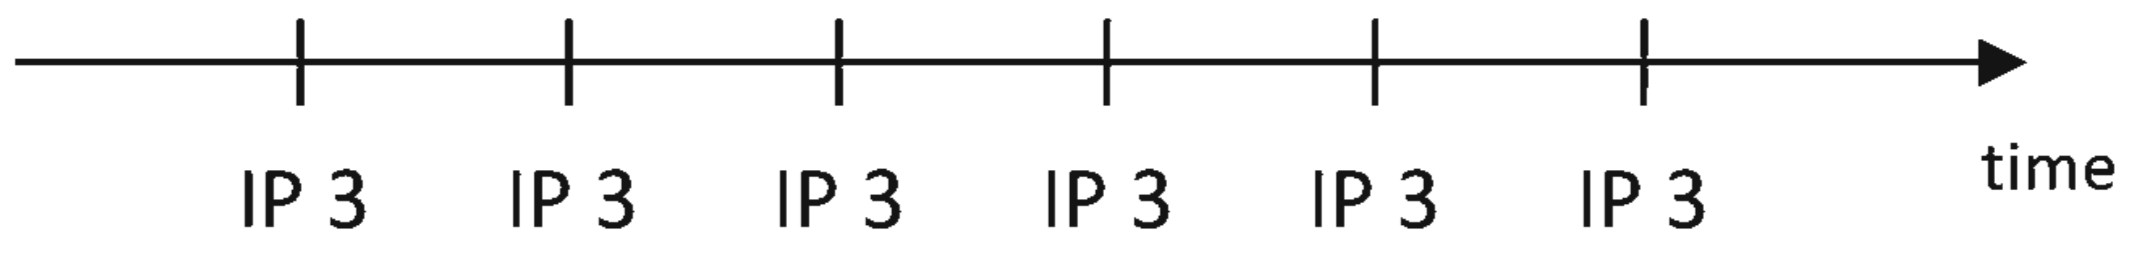
\includegraphics[width=7cm]{figures/trans-pattern2.png}}

  \subcaptionbox{模式3A 多转发者,单一重复转发者\label{fig:trans-pattern3}}
    {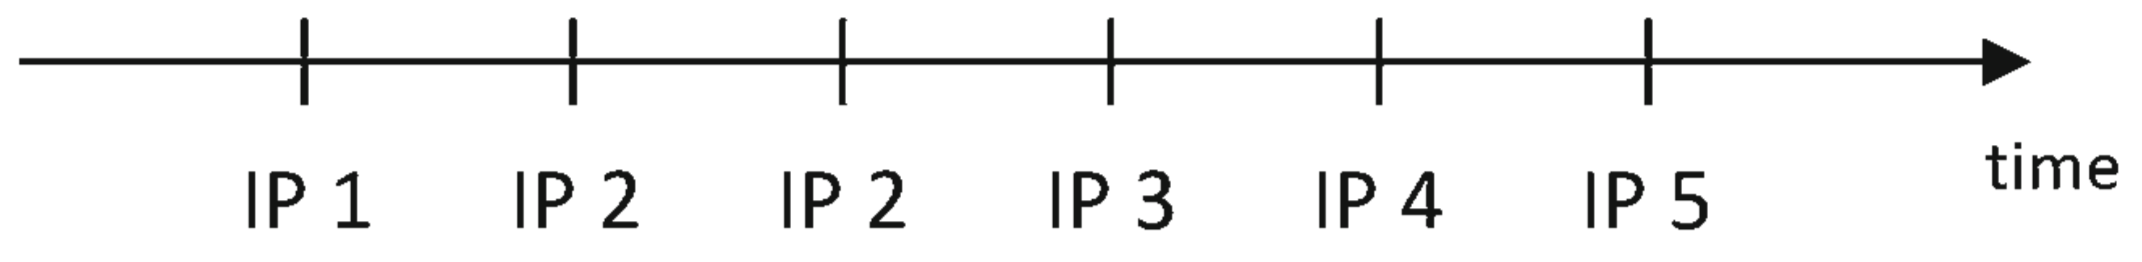
\includegraphics[width=7cm]{figures/trans-pattern3.png}}%
  \hspace{2em}%
  \subcaptionbox{模式3B 多转发者,多重复转发者\label{fig:trans-pattern4}}
  	{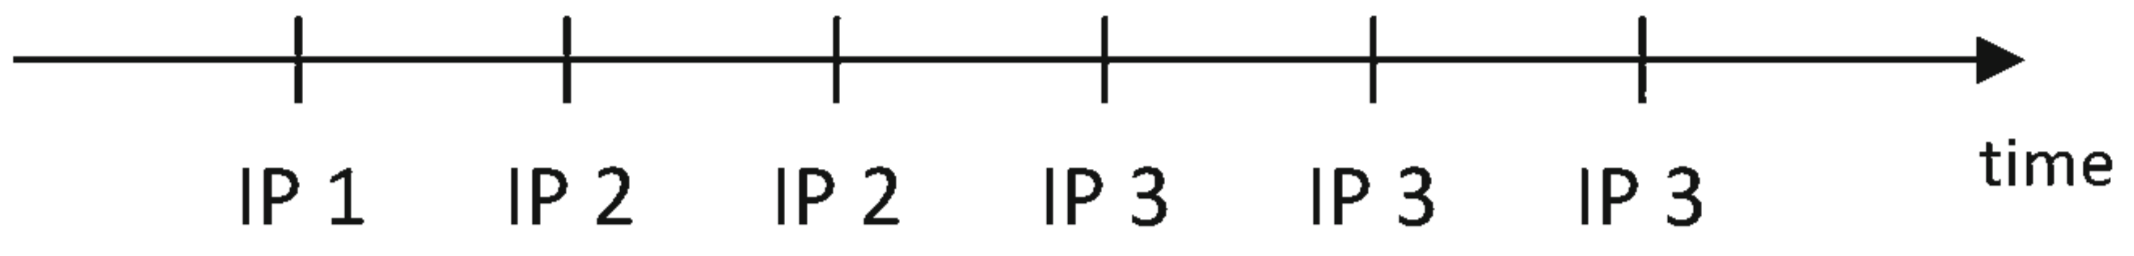
\includegraphics[width=7cm]{figures/trans-pattern4.png}}
  \caption{区块链网络中三种消息传播模式传播节点随时间的变化}
  \label{fig:trans3}
\end{figure}

2014年,Koshy等人在Kaminsky所提出假设的基础上进行了完善,归纳一段时间内监听到的消息传播情况,提出了区块链网络中消息传播的四种模式(如图\ref{fig:trans3}所示)以及对应的真实发起者假设。这一攻击方式通过监听消息传播模式,分析真实发起节点,将IP地址与消息中包含的链上地址对应,威胁通信隐私与用户身份隐私。

\begin{description}
  \item[\textbf{模式1 单一转发者}] 该模式中消息只有一个节点重复发送。在广播协议中这种情况并不常见,通常出现原因在于该节点发送不合法消息,其他节点拒绝转发该消息。因此可以假设该节点为消息实际发送者。
  \item[\textbf{模式2 多转发者,无重复转发者}] 该模式中有多个节点参与消息的转发,每个节点只发送一次。这种模式是网络中最常见的消息传播模式,在Koshy等人收集的数据中占据91。4\%。该模式中假设第一次接受到的消息发起者为消息的真实发起者。
  \item[\textbf{模式3A 多转发者,单一重复转发者}] 该模式中有多个节点参与消息的转发,除了一个节点重复多次外,其他节点只发送一次。该模式中,假设唯一的重复转发者为消息的真实发起者。
  \item[\textbf{模式3B 多转发者,多重复转发者}] 该模式中有多个节点参与消息的转发,多个节点重复发送,该模式中难以推断实际发起节点,并且所占比例较小,为2。8\%,因此Koshy等人放弃了这部分数据。
\end{description}

综上所述,区块链系统的隐私内容以及对应的攻击方式总结如表\ref{tab:privacy}所示。

\begin{table}[htbp]
	\centering  % 显示位置为中间
	\caption{区块链隐私内容及对应攻击方式}  % 表格标题
	\label{tab:privacy}  % 用于索引表格的标签
	%字母的个数对应列数,|代表分割线
	% l代表左对齐,c代表居中,r代表右对齐
	\begin{tabular}{|p{3cm}<{\centering}|p{5cm}<{\centering}|p{5cm}<{\centering}|}  
		\hline  % 表格的横线
		区块链隐私分类 & 隐私保护内容 & 隐私威胁攻击方式 \\  % 表格中的内容,用&分开,\\表示下一行
		\hline
		交易内容隐私 & 账本记录的单笔交易信息,包含交易发起方、交易接受方、交易金额以及附带数据等隐私信息 & 通过区块链钱包、浏览器等工具爬取区块链账本记录 \\
		\hline
		账户地址隐私 & 区块链地址与交易的关联关系,包含账户地址的交易记录、余额以及不同账户间交易等隐私信息 & 通过分析区块链账本记录,构建交易网络 \\ 
		\hline
		用户身份隐私 & 用户和区块链地址、交易的关联关系,包含同一用户的交易记录、资金余额等隐私信息 & 利用区块链交易特征,在交易网络的基础上构建用户网络。也从论坛、交易所等区块链服务获取 \\ 
		\hline
		节点隐私 & 节点相关信息,包含节点网络IP、软件版本、服务器系统等隐私信息 & 在区块链网络中部署节点监听或爬取其他公开信息获取 \\
		\hline
		通信隐私 & 节点间通信内容,包含节点间通信的数据内容以及通信流量情况 & 通过在区块链网络中部署监听节点,监听节点间通信进行获取 \\
		\hline
	\end{tabular}
\end{table}

\section{地址混淆机制}

区块链技术较为广泛应用于密码货币领域,由于区块链账本记录了历史上所有的交易记录,通常对网络中所有节点公开可见,因此攻击者可以通过分析账本进行攻击。账本分析攻击的基础假设1认为同一交易的所有输入地址属于同一用户。为了抵抗账本分析技术,研究者针对该技术所基于的假设,提出交换资产、混淆地址的防御机制,即地址混淆机制。不同的用户通过交易相互交换资产,这样假设1会将不同用户的账户地址误认为属于同一用户,达到混淆用户地址、保护各用户隐私的效果。由于地址混淆机制通过交换资产的方式进行,因而通常称为混币机制,用于交换资产的交易称为混币交易。

地址混淆机制有多种不同的实现形式,根据具体操作者的不同分为中心化混币和去中心化混币两类技术。中心化混币技术需要中心化混币服务提供商参与,帮助混币用户进行混币操作;去中心化混币技术由所有参与混币的用户按照协议自发进行混币交易。两类实现技术有各自的优缺点,例如中心化混币技术便于用户使用,但混币服务提供商存在安全隐患;去中心化混币技术安全性更强,但需要用户寻找混币同伴并与其他混币用户交互构造混币交易,使用不便。针对地址混淆机制中各类实现技术,我们提出以下度量指标:

\begin{itemize}
	\item \textbf{资产安全性} 经过地址混淆的操作后,用户能在约定时间之前取回自己参与混币的资产(扣除手续费)。
	\item \textbf{外部隐私性} 用户参与混币交易的输入输出地址关联关系,被外部攻击者关联的可能性。在中心化混币协议中,外部用户指除了中心化混币服务提供商以及用户本身外的其他用户;在去中心化混币协议中,外部用户指除了参与混币协议的用户以外的其他用户。
	\item \textbf{内部隐私性} 用户参与混币交易的输入输出地址关联关系,被参与混币过程的攻击者关联的可能性。
\end{itemize}

\subsection{中心化混币}

中心化混币服务提供商帮助希望进行混币交易的用户找到同伴,构造混币交易并从中收取一定额度的手续费。中心化混币技术中,混币服务提供商作为中介角色分别与各用户进行交易,接收到用户的资产后,进行随机混淆然后返回给其他用户。通过将不同用户的资产互相交换,达到混淆不同用户地址的效果,因而分析攻击只能将所有参与混币服务的地址聚类到一起,难以分辨出属于单一用户的账户地址。

\begin{figure}
\centering
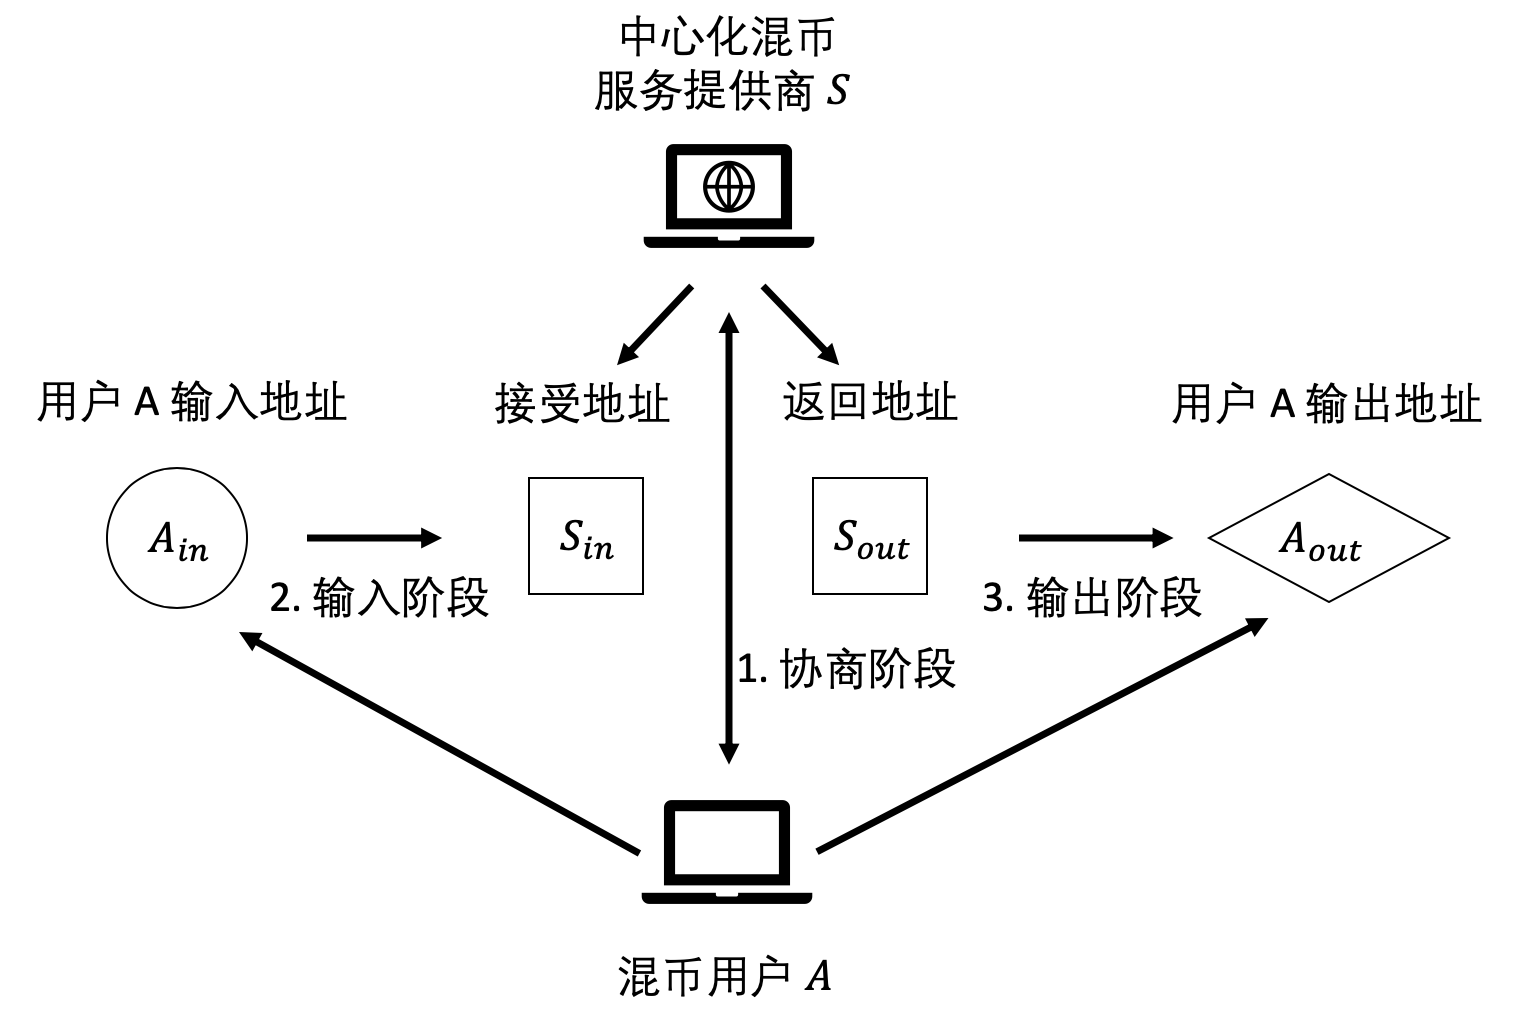
\includegraphics[height=7cm]{figures/cen-mixer.png}
\caption{中心化混币模型}
\label{fig:cen-mixer}
\end{figure}

中心化混币协议的基本模型如图\ref{fig:cen-mixer}所示,具体的协议流程主要分为协商、输入、输出及结束四个阶段:

\begin{enumerate}
	\item \textbf{协商阶段}:希望参与混币的用户与混币服务提供商进行协商,约定用户用于混币的输入地址、输出地址、服务提供商的接受地址、返回地址、混币金额、混币输入输出时间、混币手续费等相关参数。
	\item \textbf{输入阶段}:用户按照协商阶段商定的相关参数在约定时间之前将约定资产从输入地址发送到服务提供商指定的接受地址。
	\item \textbf{输出阶段}:服务提供商在约定时间之前将扣除手续费后的资产通过返回地址发送到用户指定的输出地址。
	\item \textbf{结束阶段}:若协议正常运行结束,服务提供商和用户销毁协商阶段留下的记录,保护用户隐私。
\end{enumerate}

最早的中心化混币服务例如BitLaundry平台采用最基础的中心化混币协议,用户将输入输出地址、交易金额以及交易时间等信息发送给BitLaundry,然后将对应金额的密码货币发送到BitLaundry指定的链上地址,BitLaundry确认接受后,将其他来源的对应数量货币返回到用户指定地址,并从中赚取固定手续费。这一方案的好处在于用户可以发送任意金额,并且指定交易的时间。然而BitLaundry平台的固定配置和暴露给用户的链上地址给攻击者提供了分析的机会,攻击者可以根据搜集的BitLaundry平台地址以及固定的手续费特征将混币交易提取并且关联在一起[38]。基础的中心化混币服务主要存在如下问题:

\begin{enumerate}
	\item 中心化混币服务提供商的行为存在一定特征,例如混币交易在时间上的规律,抽取一定比率的手续费,存在一个常用的地址池等等。攻击者可以通过上述特征进行混币交易的分析,将用户的输入输出地址关联起来,难以满足外部隐私性。
	\item 中心化混币服务提供商存在内部作恶的风险,无法保证在接受到用户输入资产后将对应资产返还给用户。在区块链系统中,所有链上地址都是算法生成的假名,因此用户无法证明自己的资产是否被窃取,平台也难以提供证据自证清白。此外,服务提供商也无法保证删除了用户输入输出关联关系的记录,因此不能满足资产安全性和内部隐私性。
\end{enumerate}
	
针对上述问题,研究者们提出了增加中心化混币协议外部隐私性、内部隐私性和资产安全性的相应技术。主要通过随机化机制减少混币服务提供商存在的特定行为特征,增加攻击者进行分析的难度,从而增强外部隐私性;通过要求混币服务提供商对协商阶段的参数进行数字签名作为承诺,以防服务提供商盗窃用户资产,增强资产安全性;通过在协商阶段使用盲签名技术,在保持承诺机制的前提下保护关键参数不对服务提供商可见,从而对服务提供商隐藏用户输入输出地址之间的关联关系,提供内部隐私性。

\subsubsection{随机化机制}

为了防止攻击者根据平台固定的手续费等配置来关联混币用户的输入输出地址,随机化机制通过中心化混币服务提供商在输出阶段人为制造交易时间、手续费等信息的随机性,掩盖混币交易的特征。中心化混币平台Bitcoin Fog将收取的手续费设定为一个范围之间的随机值,并在用户指定时间区间内随机挑选时间将资产返还到用户指定地址。这一方案可以减少外部攻击者根据混币特征关联用户地址的可能,在一定程度上保护用户隐私。

在实际应用中,用户为了防止中心化混币服务商泄漏用户隐私,会将资产在多家混币服务商依次进行混淆,此时连续的混币交易存在的手续费特征会暴露用户隐私。为解决这一问题,Mixcoin协议[15]设计了随机的、全有或全无(all-or-nothing)的手续费机制,混币服务提供商以约定好的概率将部分用户的混币金额全部留做手续费,其他用户的混币金额全额返还。为了保证生成随机数的可信性,Mixcoin采用约定区块链某未来区块的数据作为随机化参数,一定程度上保障随机数的不可伪造性。服务商M根据用户提供的参数 , , ,计算随机值 ,其中 表示第 个区块的交易二叉树根的值,PRNG为密码学伪随机数生成算法,根据输入参数生成(0,1)区间中对应的随机数。如果生成的随机值小于阈值,即 ,则服务商M收取所有混币资产作为手续费,否则返回全部资产。

采用随机化机制主要增强中心化混币方案的外部隐私性,防止外部攻击者通过混币交易存在的固定特征分析用户的混币过程。但不能提供内部隐私性与资产安全性,混币服务商可能盗窃用户资产或者泄漏用户地址关联关系等隐私信息。

\subsubsection{基于数字签名的承诺机制}

由于在区块链系统中,中心化的混币服务商没有实体身份作为信誉担保,可能出现盗窃用户资产的行为,用户很难相信混币服务商。同时用户的账户地址也不存在对应的身份,因而服务商难以自证清白。为了保护用户资产安全,混币服务商通过长期公钥代表身份建立承诺机制。在协商阶段,混币服务商需要提供身份对应的数字签名作为承诺。承诺包括约定的输入输出地址、混淆资产金额、约定时间等信息,并用混币服务商的长期公钥对应私钥进行签名。
	
利用数字签名技术提供不可伪造和不可抵赖的特性,增加承诺机制帮助用户证明平台的窃取行为。服务提供商通过维护自己的“虚拟声誉”,即代表身份的长期有效公钥,使得用户信任该服务商。使用该公钥对应私钥的签名向用户承诺平台不会出现盗窃行为,否则用户可以通过公开该承诺以及不符合承诺的区块链账本记录向其他用户证明该平台存在盗窃行为,破坏服务商的声誉。承诺机制一方面依靠在一定程度上保障了用户资产安全,另一方面也避免了用户恶意造谣。

\begin{figure}
\centering
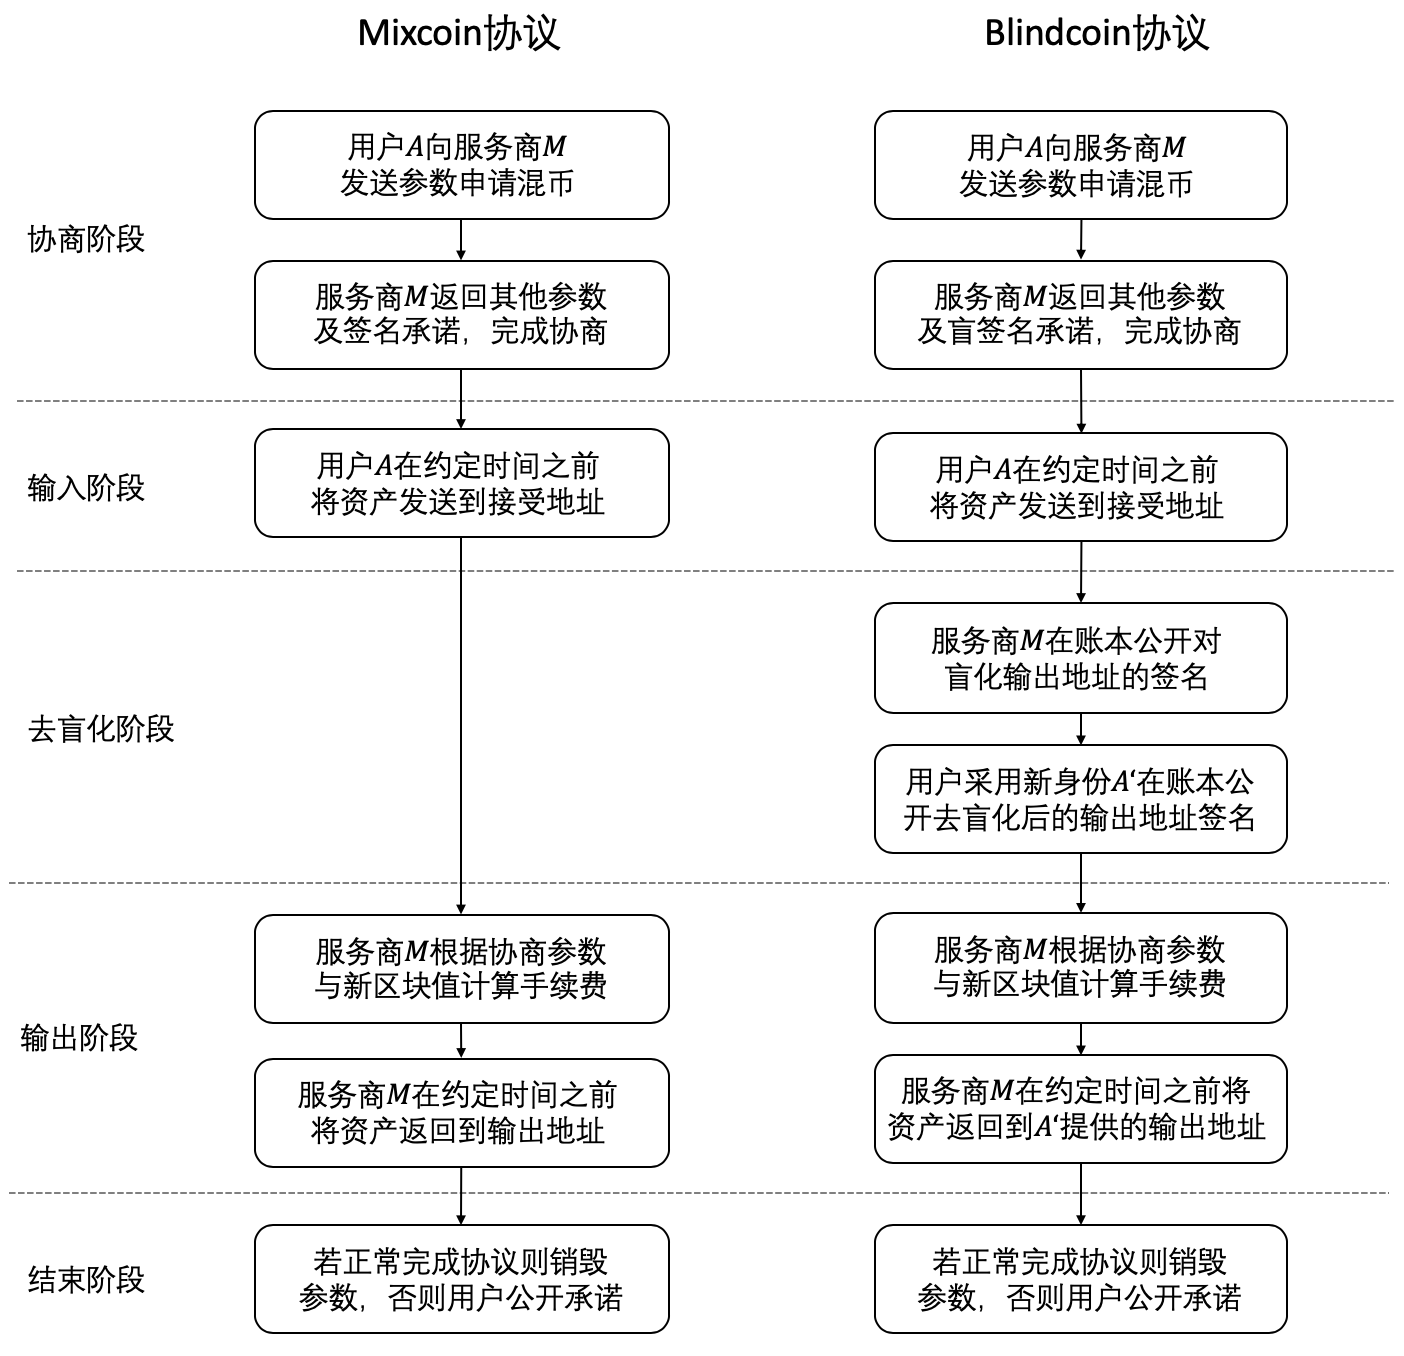
\includegraphics[width=10cm]{figures/mixcoin-blindcoin.png}
\caption{Mixcoin协议和Blindcoin协议}
\label{fig:mixcoin-blindcoin}
\end{figure}

2014年,Joseph等人提出了Mixcoin协议[15],通过基于数字签名的承诺机制增强资产安全性Mixcoin协议的核心步骤如图\ref{fig:mixcoin-blindcoin}所示,在协商阶段加入承诺机制,服务提供商需要对协商参数进行签名作为承诺,用户得到承诺后再向服务提供商支付混币资产。若服务提供商未按照承诺在约定时间之前返回资产,则用户在结束阶段可以公示在协商阶段收到的承诺与区块链账本记录的事实证明该服务提供商违背承诺。
	
Mixcoin协议通过承诺机制在一定程度上保护了用户的资产安全,但是该协议无法提供内部隐私性,即平台无法证明已如约销毁用户混币记录,用户也无法进行验证。因此用户为了保护自己的混币隐私不被恶意平台泄漏,通常采用在多个平台连续混币的方式。但这带来了较高的手续费,也留下更多的混币交易记录,给攻击者提供了更多特征进行分析。

\subsubsection{基于盲签名技术的隐藏机制}
为了提供中心化混币方案的内部隐私性,需要服务提供商在不知道用户输入输出地址对应关系的情况下进行输入和输出阶段,利用盲签名技术可以达到这一目的。1983年,Chaum等人[39]提出了盲签名的概念,盲签名技术是一种特殊的数字签名技术,在签名者对消息内容进行签名的过程中并不知道消息内容。盲签名技术满足以下两条性质,其中第一条特征保证了签名消息的内容隐私性,第二条特征保证了签名请求者的身份隐私性:
\begin{enumerate}
	\item 被签名消息对签名者是不可见的,即签名者不知道他所签署消息的具体内容。
	\item 签名消息不可追踪,即当签名消息被去盲化公布后,签名者无法将去盲化签名与盲化签名对应上。
\end{enumerate}

\begin{figure}
\centering
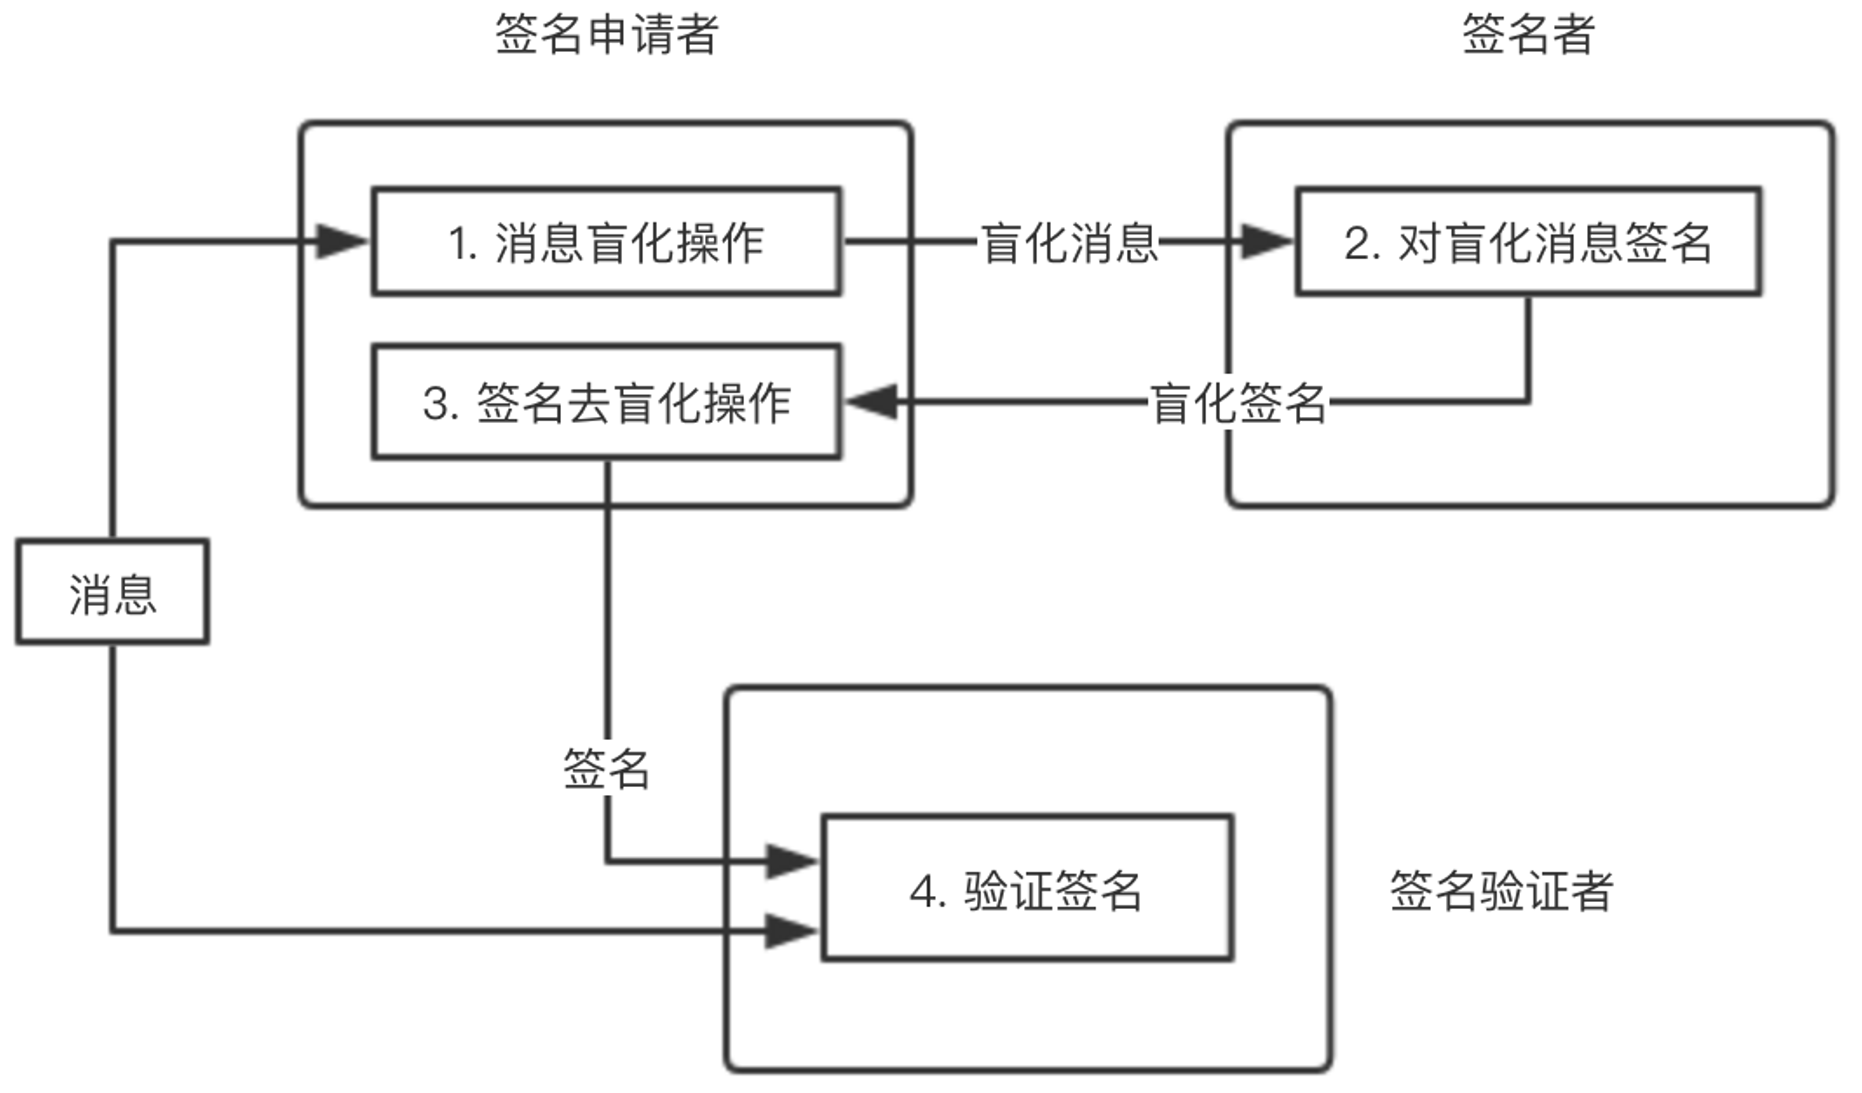
\includegraphics[width=10cm]{figures/blind-sig.png}
\caption{盲签名流程}
\label{fig:blind-sig}
\end{figure}

盲签名技术的整体流程如图\ref{fig:blind-sig}所示,主要分为以下四个步骤:

\begin{enumerate}
	\item 签名申请者首先将消息进行盲化操作,将盲化消息发给签名者。
	\item 签名者对盲化消息进行签名操作,将盲化签名返回签名申请者。
	\item 签名申请者对收到的盲化签名再作去盲变换,得出的便是签名者对原数据的签名。
	\item 签名申请者可以公布原始消息与去盲化签名,由验证者进行验证。
\end{enumerate}

2015年,Luke等人提出了Blindcoin协议[16],通过采用盲签名技术保障中心化混币方案的内部隐私性,核心步骤如图\ref{fig:mixcoin-blindcoin}所示。该协议保留了Mixcoin协议的随机化手续费、承诺等机制,并在此基础之上通过盲签名技术使得混币用户的输入输出地址关联关系对服务提供商不可见。该协议首先修改了协商阶段的签名部分,服务提供商对包含盲化的用户输出地址的承诺进行盲签名,然后用户对盲化签名进行去盲化操作得到针对真实输出地址的签名,并作为输出地址获取混币资产的凭证提交给服务商,服务商可以验证该签名的正确性以及是否使用过。由于服务商在协商阶段知道用户的输入地址但不知道输出地址,而在输出阶段知道输出地址而不知道对应的输入地址,因而无法判断用户输入输出地址的关系。盲签名技术可以有效增强中心化混币方案的内部隐私性,为了同时保持MixCoin方案中的可审计特性,该协议需要通过在公开的可信账本(论文推荐使用同一区块链)中记录下盲签名和去盲签名的内容,达到时间戳认证的效果。这一设计不会暴露用户的隐私,而一旦混币服务提供商未履行承诺,用户可以公示服务商提供的承诺,并使用在区块链账本中存储的消息作为违约证据。

\subsection{去中心化混币}

尽管中心化混币技术中系列协议在一定程度上保障了资产安全性和隐私性,但其依赖的混币服务提供商仍会带来一些潜在风险,例如遭受黑客攻击进而盗窃用户资产。研究者提出了一系列去中心化的混币协议,通过多方参与的协议代替中心化混币服务提供商,使得用户不需要先将自己的比特币发送给混币服务提供商,而是在网络中找到其他需要混币的用户,通过多方参与者运行协议的方式构造一致的混币交易,确认后签名使得交易生效。这一系列协议从根本上解决了中心化混币存在的信任问题,同时节省了混币服务提供商收取的手续费。但是也存在着一些不足,比如寻找其他混币用户存在困难,容易让外部攻击者混入并监听混币关系甚至进行拒绝服务攻击(DOS,Denial of Service)导致混币失败。
 
\begin{figure}
\centering
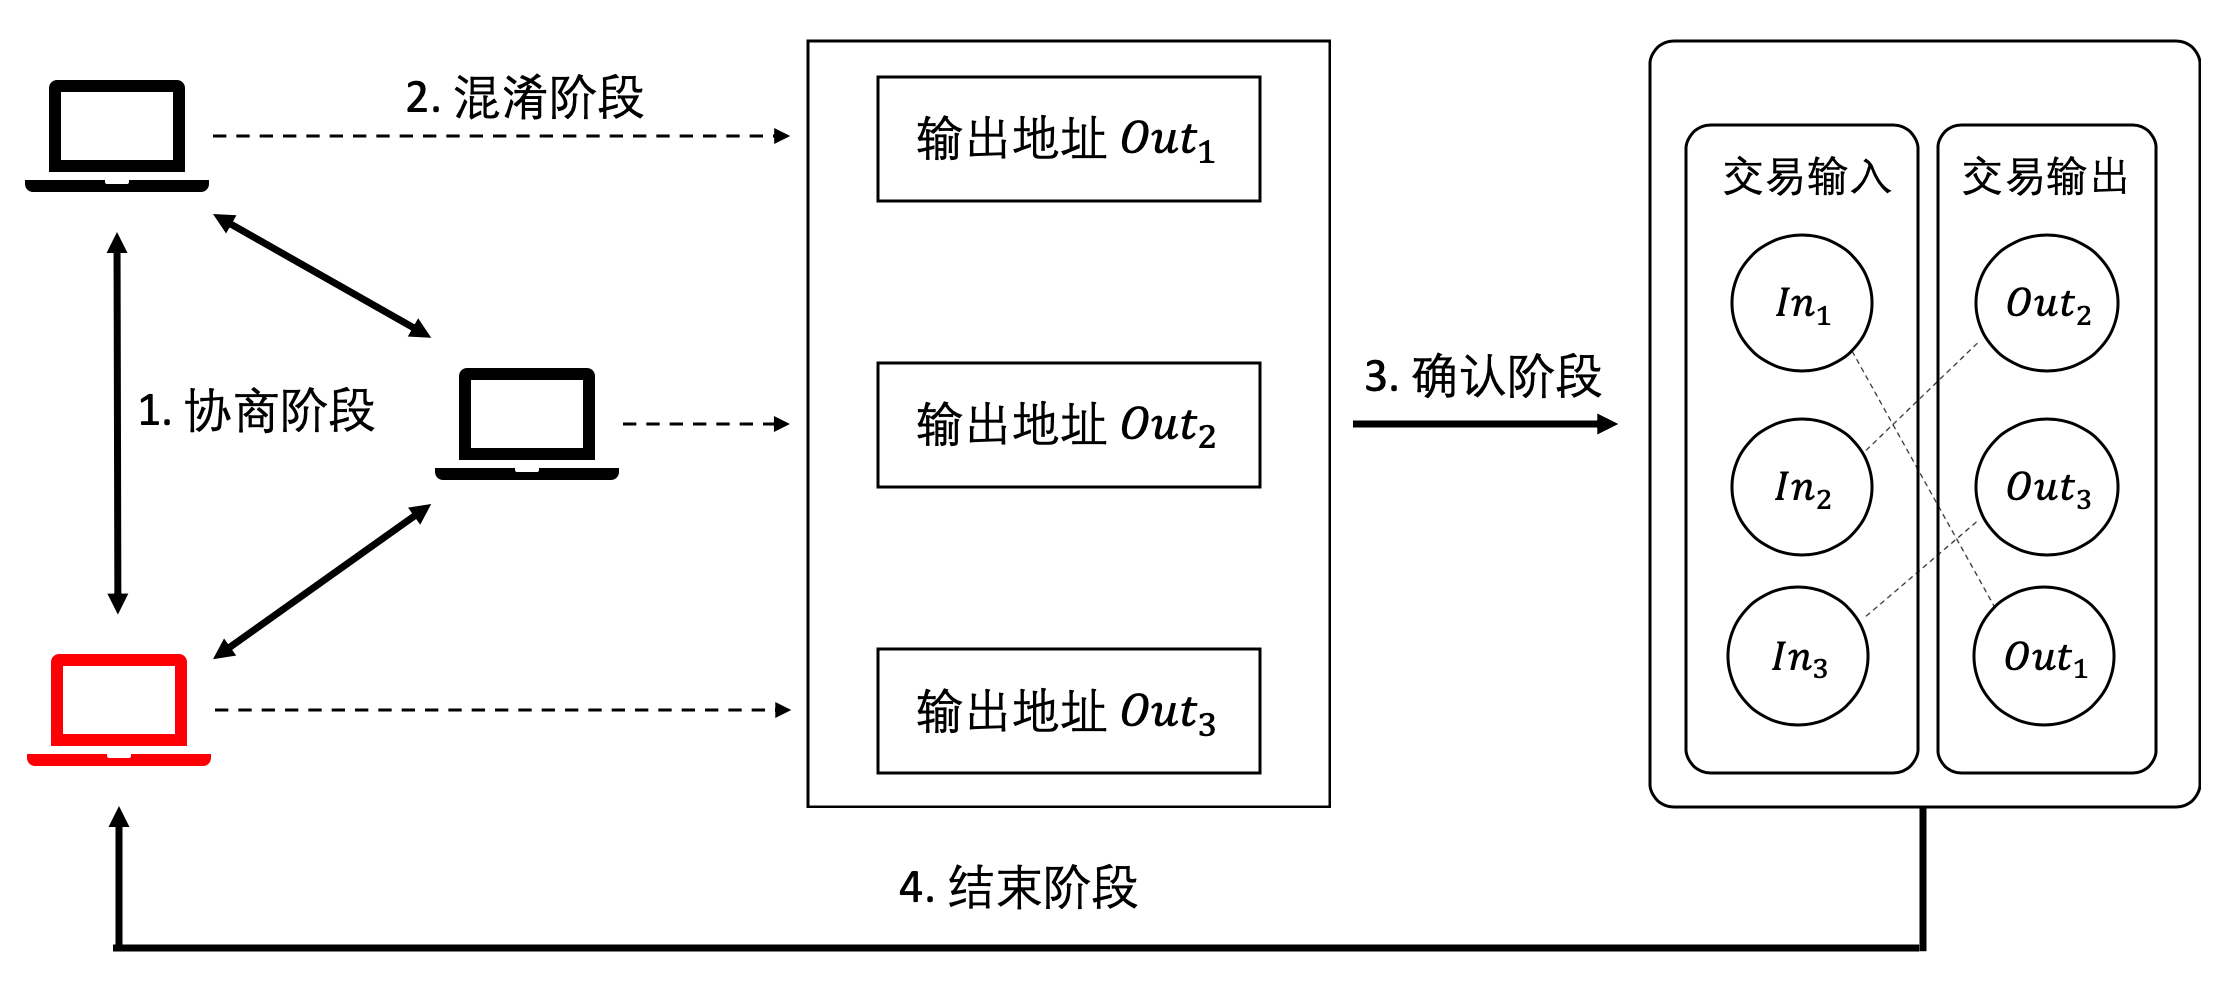
\includegraphics[width=10cm]{figures/decen-mixer.png}
\caption{去中心化混币模型}
\label{fig:decen-mixer}
\end{figure}

去中心化混币协议的基本模型如图\ref{fig:decen-mixer}所示,分为协商、混淆、确认及结束四个阶段,其中红色节点表示混入的攻击者。与中心化混币协议的区别主要在于执行的角色由中心化混币服务器转变为参与混币的用户多方共同完成:

\begin{enumerate}
	\item 协商阶段:用户寻找参与混币的其他同伴,协商去中心化混币协议需要的参数,例如各用户混币输入输出地址、混币金额等参数。
	\item 混淆阶段:参与混币的用户根据协议对所有输出地址进行混淆,隐藏用户输入输出地址之间的关联关系。
	\item 确认阶段:混币用户根据混淆阶段得到混淆后的交易输出,构造混币交易,确定无误后进行广播,将混币资产发送到各用户指定的输出地址。
	\item 结束阶段:若混币协议正常结束,参与混币的各用户销毁此次混币过程相关记录,若过程出现错误中止,参与混币的用户找出并且排除造成错误的用户。
\end{enumerate}

去中心化混币技术根据参与方的数量主要分为多方混币技术与双方混币技术两类。其中多方混币技术参与者数量大于等于3,且隐私保护程度与参与者数量成正相关。其优点在于多参与方增强了地址混淆的外部隐私性,多参与方构造一笔交易也能节省交易费。缺点在于参与者数量的上升会增大攻击者混入的概率,攻击者可以在协议过程中监听并分析其他参与者的输入输出地址关联关系,威胁内部隐私性,甚至进行拒绝服务攻击中断协议进程。双方混币技术只有两个参与方,单次混淆只能提供一定的外部隐私性,并且不能提供内部隐私性,因此双方混币技术中用户需要与不同参与方进行多轮混币来增强隐私性。优点在于提升了协议的隐私性,并且每次的混币操作简单,缺陷在于多次混币需要进行多次交易,带来了高额交易费。

\subsubsection{多方混币技术}
多方混币技术主要模型为n个参与方约定相等的混币金额,构建n-to-n的多签名交易,保证每个交易输出都为相等的金额,外部攻击者无法通过分析该交易分辨不同的输出,从而无法分析每个输出与输入地址之间的关联关系,保障外部隐私性。

\begin{figure}
\centering
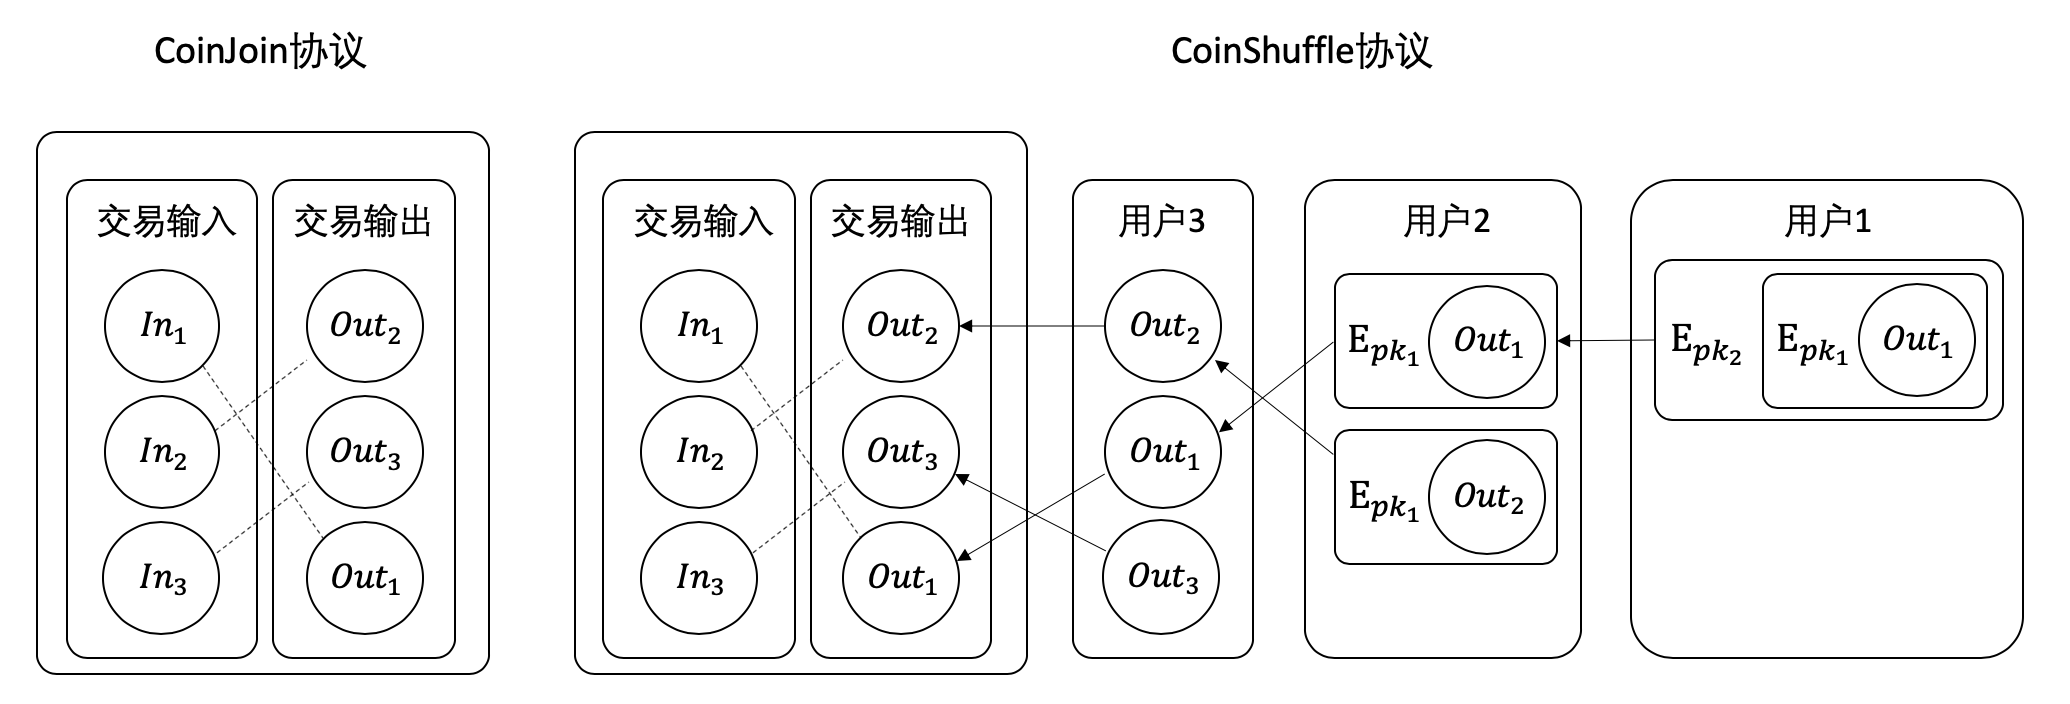
\includegraphics[width=10cm]{figures/coinjoin-shuffle.png}
\caption{CoinJoin协议和CoinShuffle协议}
\label{fig:coinjoin-shuffle}
\end{figure}

2013年8月,Gmaxwall提出了CoinJoin协议[17],如图\ref{fig:coinjoin-shuffle}所示,该协议在协商阶段由参与混币的用户协商输入输出地址、统一输出金额等参数,然后在混淆阶段将所有输入和输出放入同一交易中构造混币交易,确认阶段中,各参与者检查自己的输出无误后对输入进行签名,当所有参与用户完成签名后将该交易广播到网络中。这一协议操作十分简单,参与用户无需信任其他节点,也不用缴纳混币手续费,攻击者无法分辨n个金额一致的输出资产,保障协议的外部隐私性。并且用户可以先检查混币交易中自己的输出地址与金额是否正确,然后决定是否对交易输入进行签名,提供了资产安全性。但是,CoinJoin协议的缺陷在于协商阶段中参与用户的输入输出地址关联信息会被其他参与混币的用户获取,不能提供地址混淆的内部隐私性。此外,一旦参与混币的部分节点拒绝签名或者提前花费参与混币的输入资产,会导致混币失败。因此内部隐私性不能得到保障。

基于CoinJoin协议的Dash项目[3]在此基础上进行一定的改进,该项目中的混币交易由网络中的主节点构造保证了内部隐私性。多个主节点为用户的交易进行链式混币,上一个主节点的交易输出作为下一个主节点的交易输入进一步混淆,为了便于不同金额的交易进行,Dash将所有金额拆分为十进制单位的和。由于每次混淆交易要求至少3位参与者,因此随着混淆链的增长,混淆集合的用户数量呈指数上升,极大增强混淆能力。也保证了只要攻击者不能控制混淆链中大部分的主节点,就难以判断用户的输入输出地址的对应关系。

除了Dash中引入主节点的方案外,为了解决CoinJoin方案中的地址关联关系泄漏问题,保障地址混淆的内部隐私性。2014年,Tim等人提出了去中心化混币协议CoinShuffle[18],该协议继承了CoinJoin的思想,使得多个混币参与者共同发起同一输出金额的交易,并且参与者可以检查交易后再签名以确保资产安全性。此外,该协议借鉴了可审计的匿名群组消息传递协议Dissent[40],采用多层加密隐藏输入输出地址的关联关系,提供内部隐私性。如图\ref{fig:coinjoin-shuffle}所示,在混淆阶段中,各用户按照一定顺序进行排列,用户1将自己输出地址通过用户n到用户2的公钥依次进行加密,得到多层加密结果,然后发送给用户2。各用户将接受到的地址集合中各地址用私钥进行解密,然后加入自己多层加密后的输出地址,发送到下一个用户。最后用户n解密得到其他所有用户的输出地址并加入自己输出地址进行混淆。混淆过程中,除了用户n以外的用户不能得知其他用户的输出地址明文,而用户n也无法得知其他用户与输出地址的对应关系,保障了内部隐私性。CoinShuffle协议的优点在于通过多层加密提供了内部隐私性,同时也继承了CoinJoin的外部隐私性和资产安全性。缺陷在于该方案的混淆阶段计算量较大,花费时间较长,并且需要所有用户同时在线。尽管设计了问责阶段发现进行错误行为的参与者,但也可能遭受攻击者的拒绝服务攻击,一旦遭受拒绝服务攻击则需要重新进行大量计算。此外,CoinShuffle协议构造的交易通常存在输出地址为输入地址两倍并且一半输出金额相等的特征,因此攻击者可以利用该特征找出CoinShuffle协议构造的交易并且将另一半找零地址与各输入地址关联[41]。

\begin{figure}
\centering
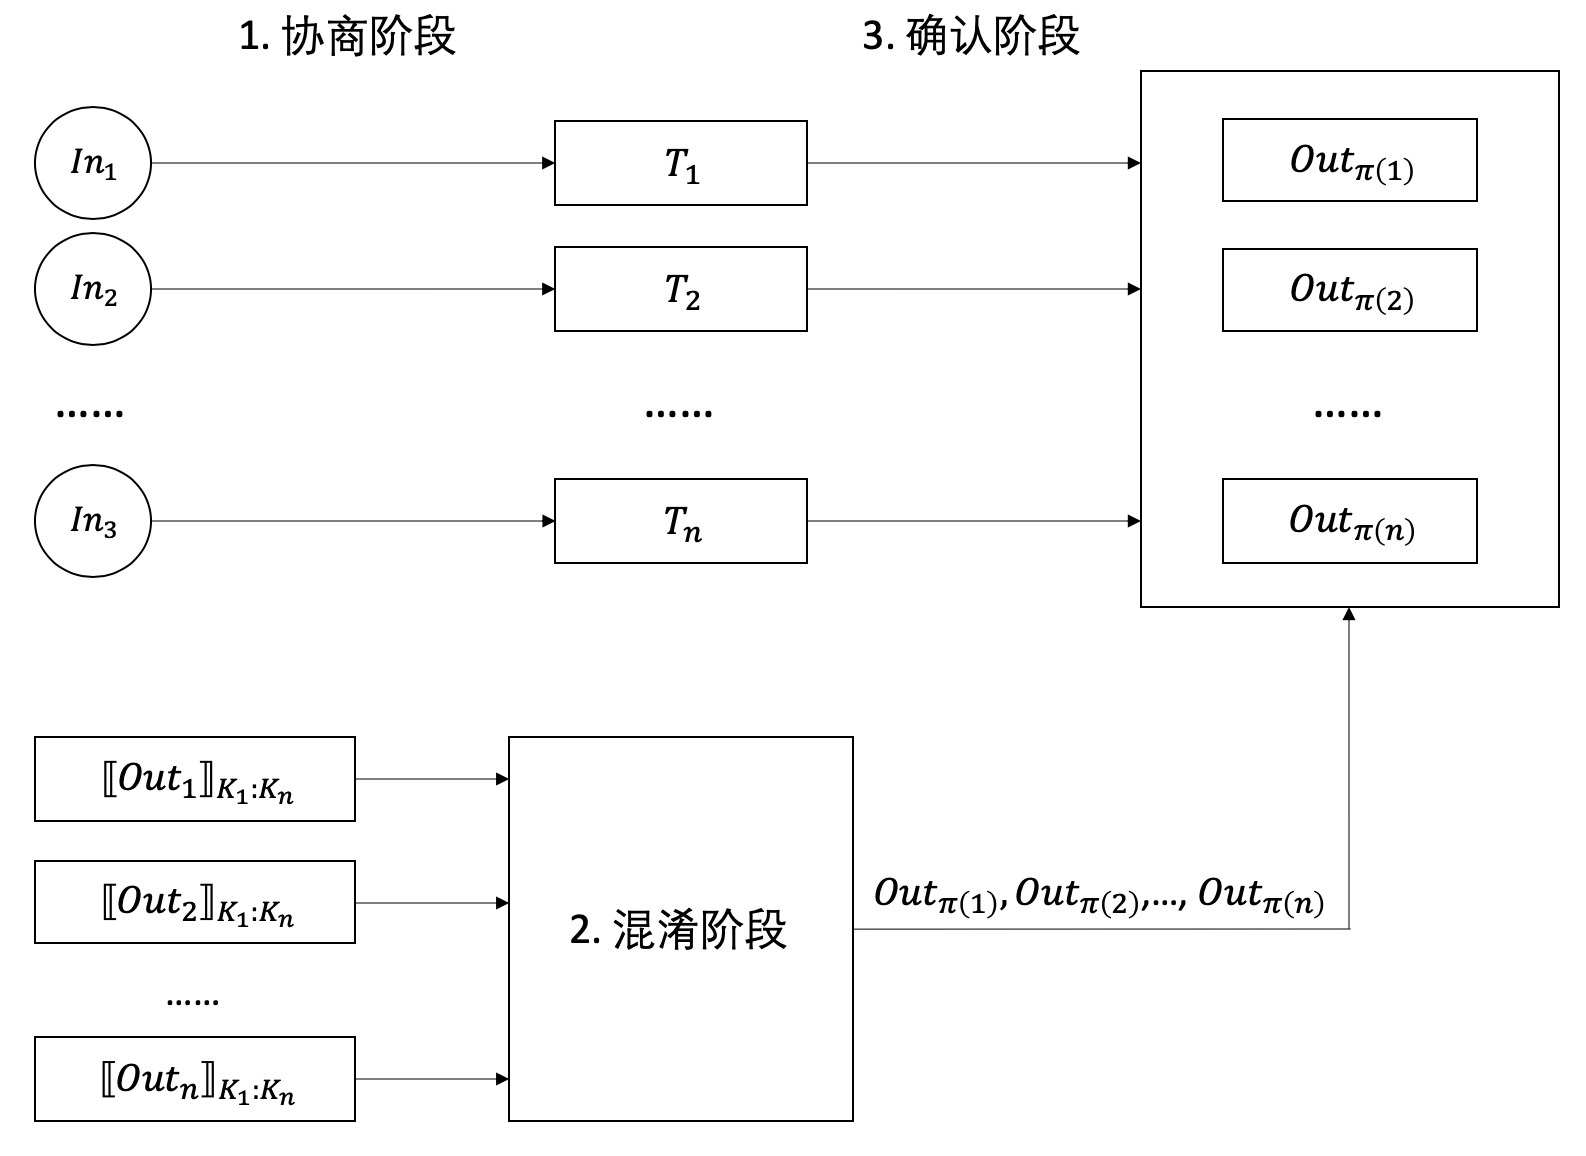
\includegraphics[width=10cm]{figures/coinparty.png}
\caption{CoinParty协议}
\label{fig:coinparty}
\end{figure}

为了解决CoinShuffle协议中混淆阶段遭受拒绝服务攻击损失较大的问题, 2015年,Jan等人提出基于安全多方计算技术的去中心化混币协议CoinParty[19],在协商阶段中,通过构建门限托管账户,接受参与者的输入资产作为抵押,增加了攻击者在混淆阶段进行拒绝服务攻击的成本。当攻击者数量较少时,正常参与的混币用户可以保障协议正常进行。CoinParty协议具体流程如图\ref{fig:coinparty}所示,在协商阶段各参与者将混币金额转入各自的临时托管地址作为抵押,表示承诺加入混币过程。临时托管地址由所有参与者通过伪随机秘密分享协议(PRSS,Pseudo-Random Secret Sharing)[42]共同生成,并需要大部分参与者共同签名才能使用,所以参与者无法独自取回抵押资产。完成协商后,CoinParty协议的混淆阶段将各参与者的输出地址进行混淆,与CoinShuffle协议同样采用了多层加密保障内部隐私性,但在CoinShuffle的基础上主要进行了两点改进,一方面采用秘密分享的校验和对比所有输出地址哈希值的和,对混淆结果进行校验;另一方面,CoinShuffle协议中最终的混淆结果由最后一位参与者决定而非随机决定,攻击者可以控制顺序。CoinParty协议以校验和作为伪随机数生成器的依据生成公共随机置换,要求最后一位参与者以字典序排序,再增加公共随机置换得到最终混淆结果,避免最后一位用户操纵排序结果。确认阶段中所有用户一同将各托管地址中存放的资产发送到混淆后对应的输出地址,即使少部分攻击者拒绝参与的情况下正常用户也能完成确认过程。

CoinParty协议的安全性保证在攻击者数量小于总参与者数量1⁄3的情况,但是在没有身份认证的情况下,攻击者可能进行女巫攻击[43],通过布置达到总参与者数量2⁄3的节点参与CoinParty协议,可以盗窃其他参与者的资产。因此该协议能提供内部隐私性和外部隐私性,但资产安全性存在一定风险。

\subsubsection{双方混币技术}

多方混币协议构造过程较为复杂,恶意攻击者加入后发布错误信息或中途退出会导致混币交易构造失败,因此容易受到拒绝服务攻击。而该类协议的隐私保护程度与混币交易参与者数量成线性正相关,为了增强外部隐私性希望加入更多参与者,但同时参与方越多也越容易引来恶意攻击者参与,给用户隐私以及混币成功率带来风险。为了防止恶意攻击者参与混币,研究者提出将单次混币操作限定在两个用户之间进行,降低恶意攻击者混入的概率,也减小攻击者攻击的危害。双方混币协议的核心思想在于将多个参与者进行一次混币交易改为混币用户多次寻找不同的混币同伴进行多轮双方混币,最终达到相同外部隐私性的混币效果。这类协议的优点在于攻击者为了获取用户资产流动,必须参与该用户的每一轮混币,但这概率上难以达到,从而减少了攻击者的威胁。缺陷在于多轮混币需要在区块链账本上发布多次交易,增加了交易费的支出,也带来了额外的时间花费。由于只有两个用户参与混淆,因此双方混币技术不存在混淆阶段。

2013年,Gmaxwall提出了CoinSwap协议[20],通过借助第三方用户作为中转隐藏交易直接输入方与直接输出方之间的关联。该协议通过第三方中间用户进行转账并保障资产安全。为了在无信任的情况下保障用户进行诚实的行为,协议中利用区块链系统中的哈希时间锁定合约(HTLC,Hashed Timelock Contract)保证参与各方的资产安全。哈希时间锁定合约包含哈希锁定与时间锁定,用户可以提供合约中哈希值的哈希原像作为私密值解锁资产,也可以在锁定时间之后使用地址签名解锁资产。哈希锁用于交易接收方接收资产,时间锁用于发起方在发生异常的情况下,一定时间后取回资产。
 
\begin{figure}
\centering
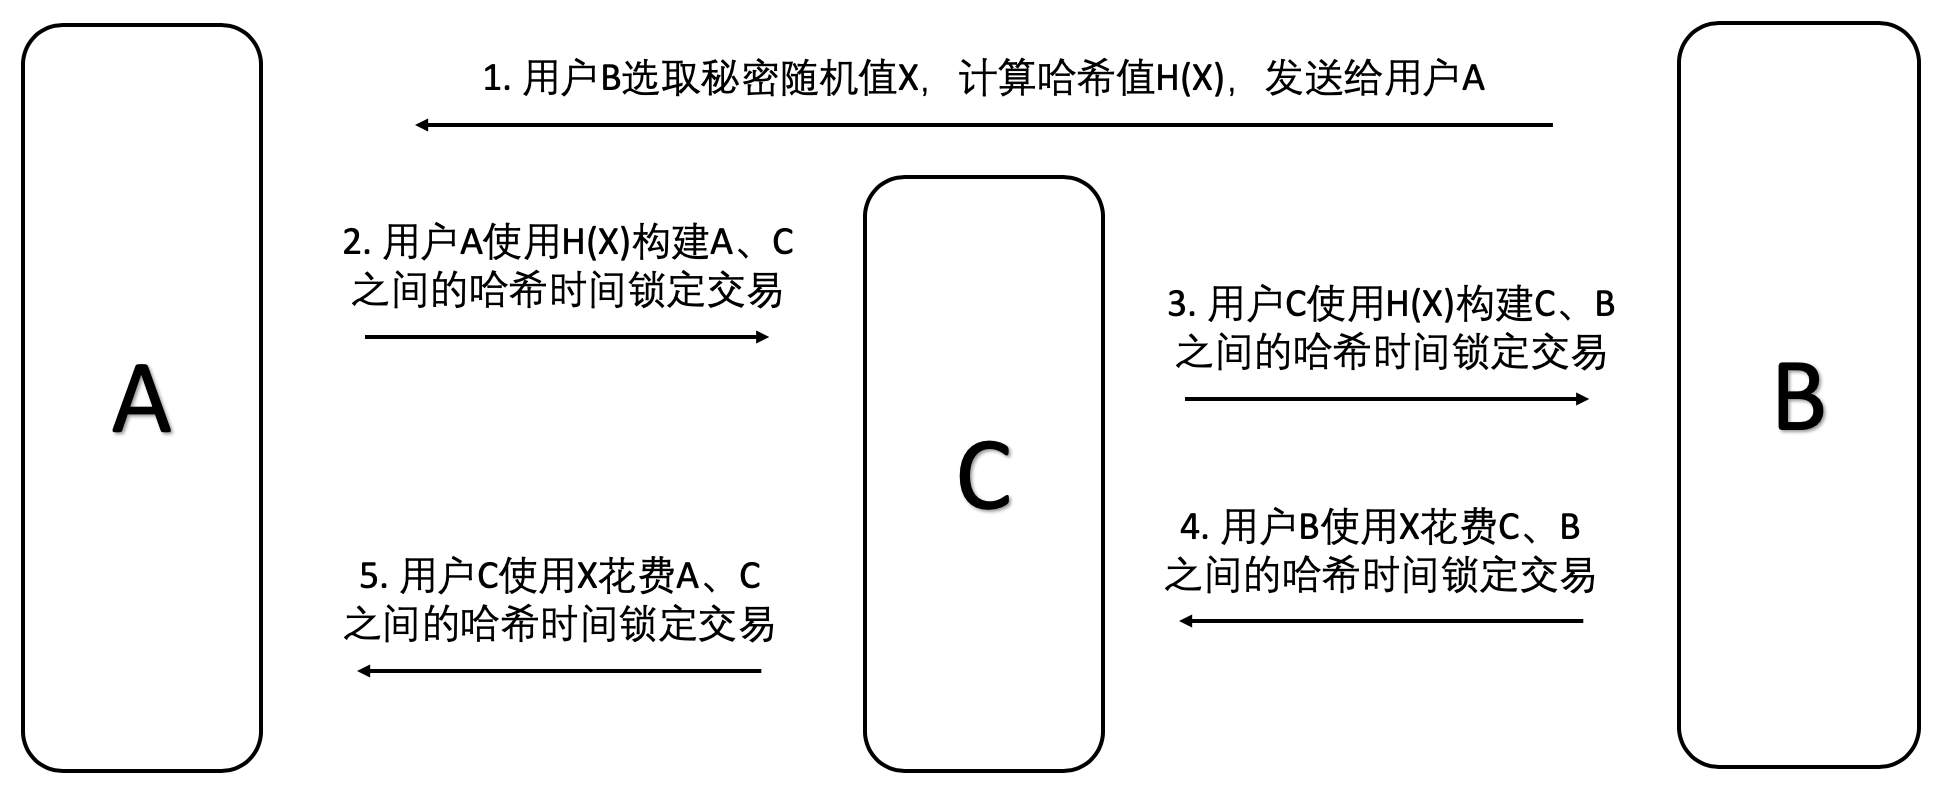
\includegraphics[width=10cm]{figures/coinswap.png}
\caption{CoinSwap协议}
\label{fig:coinswap}
\end{figure}

CoinSwap协议流程如图\ref{fig:coinswap}所示,混币交易并非构造在同一交易中,而是先由用户A向用户C发起交易,再由用户C向用户B发起交易。为了保证资产安全,该协议中的交易采用哈希-时间-签名锁,其中哈希锁利用用户B持有的私密值保证在用户B发布私密值获取资产后,用户C得知该私密值才能获取相应资产,签名锁保证用户B不能仅靠私密值获取用户A发给用户C的资产,同时采用时间锁保证在其他用户离线的情况下用户能取回自己的资产,防止拒绝服务攻击。由于用户A和用户B可以由同一用户扮演,因此该协议也可以用于双方混币。CoinSwap协议的优点在于通过哈希-时间-签名锁定合约能在无第三方参与的情况下完成混币,减少了攻击者参与的可能性,同时保障各参与用户的资产安全。缺陷在于至少多次交易带来的额外交易手续费以及两阶段交易构造与解锁带来的更长交易确认时间。

CoinSwap协议通过减少单次混币参与者数量,在一定程度上解决了攻击者监听和拒绝服务攻击的问题,但是仍存在一定隐私风险,攻击者可以通过女巫攻击的方式,尽可能多的布置混币节点,参与混币过程,攻击用户隐私安全。为了更进一步防止攻击者加入混币交易,2014年,George等人提出了能抵抗女巫攻击的去中心化混币协议Xim[21]。

Xim方案在协商阶段采用登记广告的方式构建同伴发现算法(见算法1),在公开的消息记录账本中发布广告与留言寻找混币同伴,需要支付一定的广告费,回应广告也需要支付一定手续费,用户从所有回应的用户中随机挑选同伴。因此,同时参与Xim混币的用户越多,攻击者为了让目标用户选择自己作为混币同伴,必须支付大量广告费,攻击代价随着参与Xim混币的用户数量线性增加,因而该协议能有效抵御女巫攻击。在混淆阶段,Xim协议中采用Barber等人提出的FairExchange协议[44]。Xim协议通过手续费机制提高攻击者进行女巫攻击及拒绝服务攻击的代价。此外,Xim协议的混淆范围包含当时参与Xim协议的所有参与者,极大提升了混币交易的外部隐私性。

综上所述,通过混淆账户地址保护用户隐私的机制有多种不同的技术实现。本文从协议中心化程度、资产安全性、隐私性、手续费等多个方面对介绍的协议进行了对比分析。如表3所示:

\section{信息隐藏机制}

地址混淆机制能在一定程度上保护账本隐私,但是地址混淆的结果仍会在公开账本中存储,攻击者可以通过分析带有特征的混淆交易一定程度上威胁用户隐私。为了增强隐私性,研究者们尝试将区块链账本中记录的信息包括交易发起者、交易接受者、交易金额等进行加密隐藏。另一方面,攻击者可以直接在区块链网络中监听节点信息以及通信情况,将链上内容与节点的真实情况关联,威胁用户网络隐私,可以通过隐藏网络节点信息和节点间流量来保护网络隐私。目前主要的信息隐藏技术主要隐藏以下几类隐私信息:

\begin{itemize}
	\item 交易发起者地址:区块链账本中交易的发起者地址信息,可以达到隐私保护不可追溯性,攻击者不能得到某交易发起的用户信息,保障发起者隐私。
	\item 交易接受者地址:区块链账本中交易的接受者地址信息,可以达到隐私保护不可关联性,攻击者不能将同一用户接受的两笔交易进行关联,保障接收者隐私。
	\item 交易金额:区块链账本中交易的具体金额信息。
	\item 网络节点信息:区块链网络中节点之间直接连接,需要隐藏消息发布节点的IP等信息。
	\item 网络节点间流量:区块链网络中节点间的信息流量情况,攻击者可以通过分析当前网络中流量攻击节点隐私,因此需要隐藏网络节点间流量。
\end{itemize}

信息隐藏机制的主要优点在于采用密码学加密技术提供了较高的数据隐私安全性。此外,相较于地址混淆机制,用户不需要寻找其他混淆用户进行合作。缺陷在于更大的计算量和存储空间要求。根据隐藏信息的内容,主要可以分为账本信息隐藏技术和网络数据隐藏技术,其中账本信息隐藏技术针对保护区块链账本中记录的信息包括交易发起者地址、接受者地址以及交易金额,保护账本隐私信息。而网络数据隐藏技术主要针对保护区块链网络中的节点信息以及节点间流量,保护网络隐私信息。

\subsection{账本信息隐藏}

账本信息隐藏主要防范区块链账本公开带来的账本分析攻击,通过对账本中隐私数据进行加密,保护账本隐私。并且通过密码学技术提供“凭证”,保持区块链账本正确性的可验证。现有的账本信息隐藏机制的实现技术大多属于零知识证明技术[45],零知识证明即除了所讨论命题的正确性之外不传达任何其他知识的证明。零知识证明协议中存在两种角色:证明者和验证者,证明者向验证者提供证据证明某命题成立,但不泄露除结论外的其他任何信息,验证者需要验证该证明的正确性。因此零知识证明协议需要满足三个重要属性:

\begin{enumerate}
	\item 完整性:如果证明者能证明命题成立,那么他能提供证明说服验证者。
	\item 可靠性:如果证明者不能证明该命题成立,那么他不能伪造证明欺骗验证者。
	\item 零知识性:在验证者验证证明的过程中,不能得到除了命题正确性以外的任何信息。
\end{enumerate}

相关研究者提出了许多具体零知识证明方案。例如哈密顿回路[46]和三着色问题的零知识证明方案[47]等。具体的解决方案根据应用场景不同各有差异,可以根据证明者和验证者是否需要交互分为“交互式零知识证明”(IZK, Interactive Zero-Knowledge Proof)和“非交互式零知识证明”(NIZK,Non-Interactive Zero-Knowledge Proof)[48]两类。目前在区块链领域中应用非交互式零知识证明技术,证明者可以随时独自构造并发起交易。

账本数据隐藏技术的主要衡量指标包括以下几点:

\begin{itemize}
	\item 隐藏内容:隐藏账本中的隐私数据,主要包括交易发起地址、接受地址、金额等内容。通常账本数据隐藏技术能保护其中一类内容,区块链系统通过同时采用多种技术保护多类隐私数据。
	\item 计算复杂度:构建交易和验证交易正确性的计算复杂度。由于采用了较为复杂的密码学技术进行加密和验证,因此账本数据隐藏技术给交易的构造和验证都带来了较大的计算复杂度。
	\item 空间复杂度:交易在区块链账本中占据的空间大小。采用账本数据隐藏技术构建的交易,为了证明正确性需要附带凭证,比直接保存原始数据带来更大的空间开销。
\end{itemize}

\subsubsection{密码累加器技术}

为了判断一个数据是否在某一集合中,传统的解决方案包括逐个比较,二分法查找等,这些算法的时间复杂度和空间复杂度都随着集合的增大而增加。为了解决这一问题,1993年,Benaloh等人[49]提出了“累加器”的概念,通过将整个集合组合到一个较小的累加器数据中,达到以固定大小的证据证明某元素在累加器中的效果。然而这一累加器不能从中删除元素。为了解决这一问题,2002年,Camenisch等人[50]提出了“动态累加器”的概念,基于非对称加密体系RSA[51]构造了能动态增删元素的累加器。同时,为了让用户在证明累加器中某元素存在性的同时不暴露具体元素,该研究构造了动态累加器的零知识证明。 
 
\begin{figure}
\centering
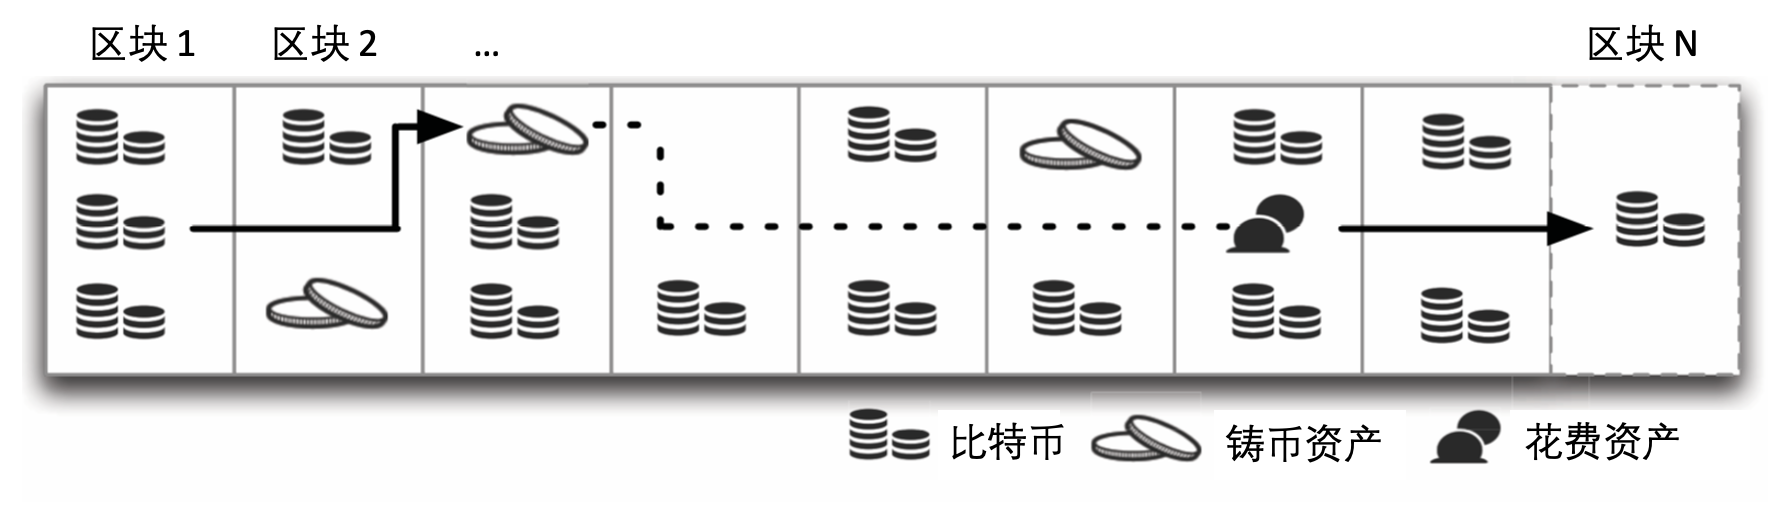
\includegraphics[width=10cm]{figures/zerocoin.png}
\caption{ZeroCoin账本示意图}
\label{fig:zerocoin}
\end{figure}

为了抵抗区块链账本公开带来的账本分析攻击,2013年,Miers等人基于比特币系统提出了ZeroCoin协议[22],这一协议如图\ref{fig:zerocoin}所示,用户可以独自进行混币操作,通过铸币交易将资产加入密码累加器,生成私密资产,达到和所有使用ZeroCoin的用户共同混币的效果。当用户需要使用之前加入累加器的资产时,根据参数生成凭证,证明自己拥有累加器资产集合中的某一未曾花费过的资产,花费该资产生成等额比特币。ZeroCoin的优点在于节点可以通过验证花费资产是否存在累加器中以及是否使用过来验证交易是否合法,但不能将用户使用的资产和此前的铸币交易对应,这样用户就完成了和整个资产集合的混淆,攻击者无法分析该资产的关联关系。并且用户可以独立完成混币交易的构造,不需要依赖任何混币服务提供商,也不需要寻找其他混币用户。攻击者无法根据用户生成的参数关联用户的铸币地址和花费地址。然而,ZeroCoin的缺点主要有三点:第一点是计算资源和交易体积的增加,这导致区块链账本的交易容量更小,也导致区块链系统性能下降;第二点是算法的初始全局参数需要可信第三方来生成,但这在公有链系统中很难得到用户的信任;第三点是无法隐藏交易金额,因此为了保护隐私,规定所有铸币和花费操作都只能使用固定值的资产,实际使用中并不方便。

\subsubsection{零知识证明技术}

简明非交互式零知识证明(zk-SNARK,zero-knowledge Succinct Non-interactive ARguments of Knowledge)技术在非交互式零知识证明证明技术的基础之上进行优化,保持非交互性的同时,减少了证明大小,节省存储空间与验证时间。该技术主要应用于可验证计算领域。zk-SNARKs技术主要由密钥生成算法、证明生成算法和证明验证算法组成。其中密钥生成算法由初始化参数生成证明密钥pk和验证密钥vk;证明生成使用证明密钥pk生成对声明x和证据a的证明 π;证明验证算法使用验证密钥验证声明x的证明 π 是否正确。该技术满足以下特征:

\begin{itemize}
	\item 完备性:对任意正确的声明x,持有证据a的证明者能生成正确的证明 π,使验证者验证其正确性。
	\item 简明性:正确生成的证明 π 空间复杂度为常数,证明验证算法的时间复杂度仅与声明x的长度成线性相关。
	\item 不可伪造性:不知道证据a的证明者无法生成正确的证明 π。
	\item 完美零知识性:验证者除了判断声明x正确性以外不能获取任何信息。
\end{itemize}

2013年,Parno等人[52]提出实现zk-SNARKs的Pinocchio 系统,该系统先将计算拆分为一阶线性约束等式(R1CS, Rank-1 Constraint System),然后转换为多项式运算形式(QAP,Quadratic Arithmetic Programs),将计算的验证转换为对多项式等式的验证,通过对点的抽样计算完成对整个多项式等式正确性的检验,基于椭圆曲线的双线性对性质隐藏用于计算的真实输入,利用可信创始方初始化阶段生成的参数实现零知识证明。该实现的安全性依赖于QAP问题的不可计算。

\begin{figure}
\centering
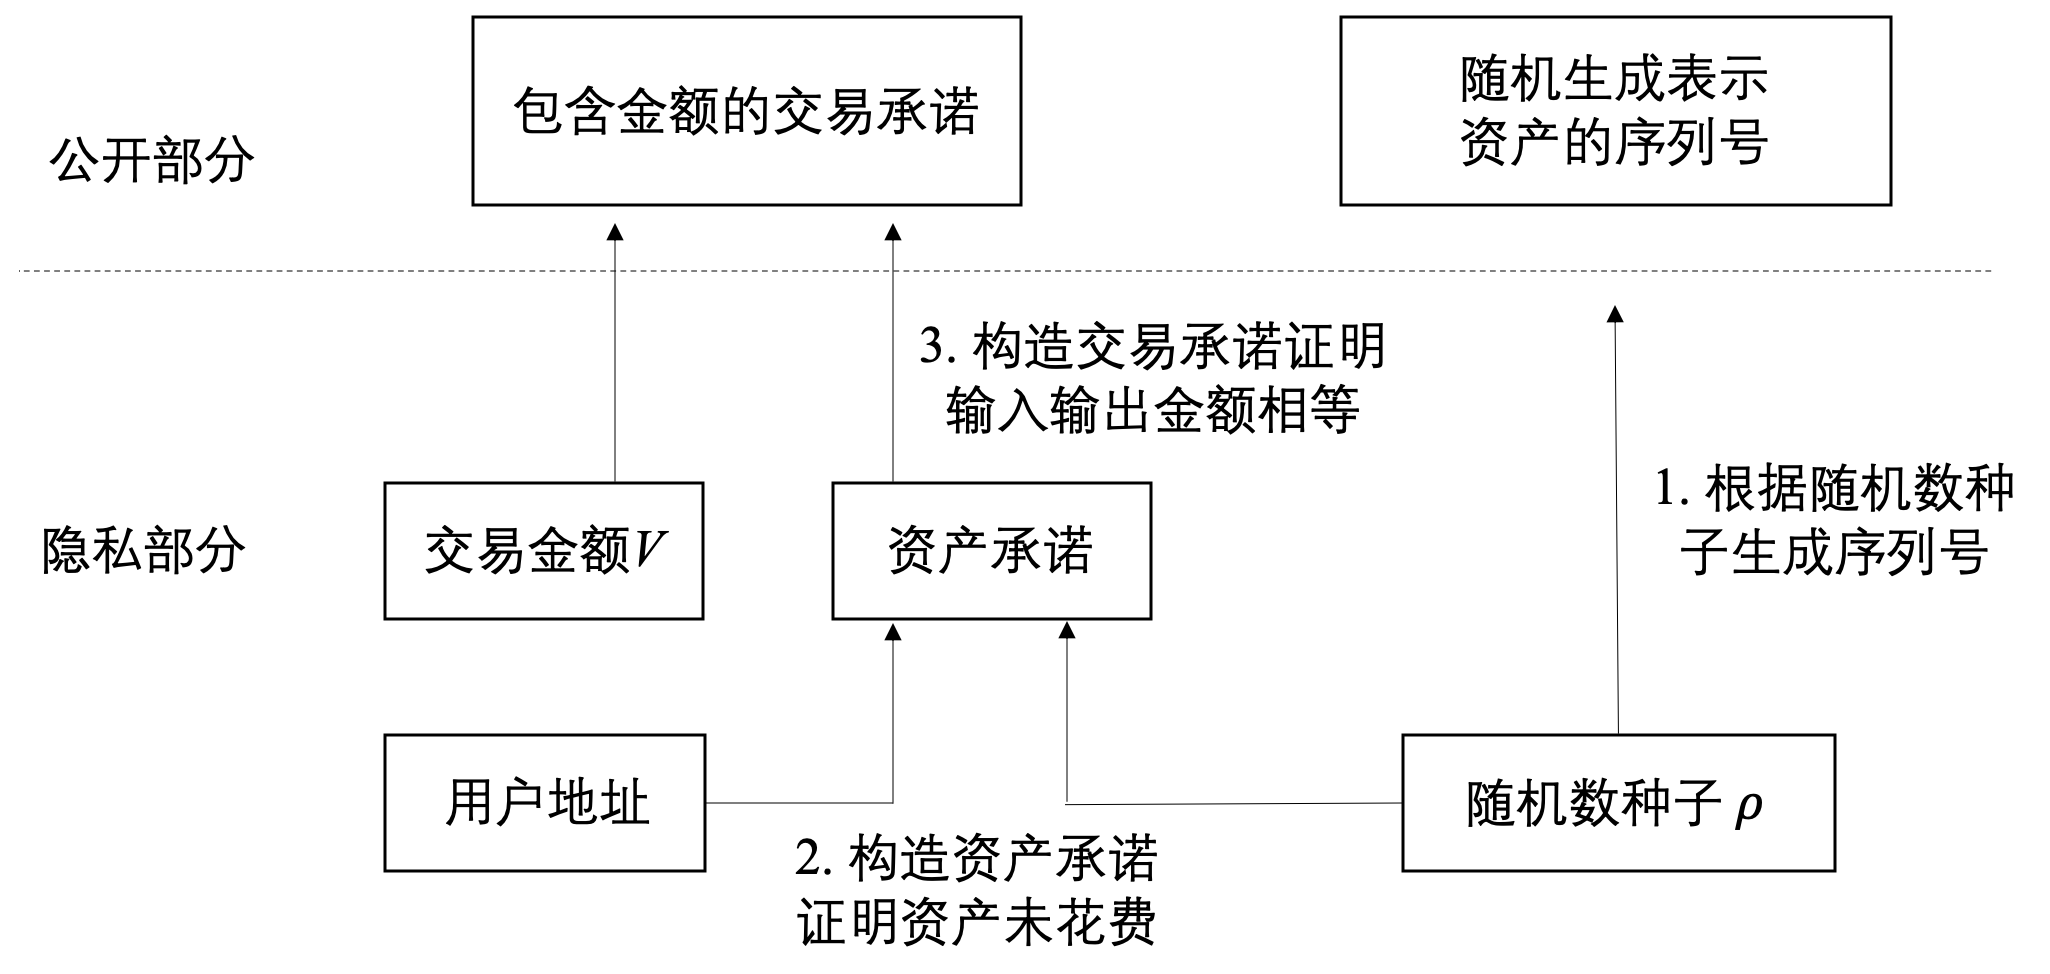
\includegraphics[width=10cm]{figures/zerocash.png}
\caption{ZeroCash协议中铸币交易的构造过程}
\label{fig:zerocash}
\end{figure}

2014年,Eli等人基于Pinocchio系统提出ZeroCash项目[23],该项目利用Pinocchio系统实现的zk-SNARKs技术构造交易。用户可以隐藏交易的发起者、接受者、交易金额等隐私信息,验证节点仍可以直接验证交易正确性。该协议与ZeroCoin同样包含铸币交易与花费交易,通过销毁资产生成私密资产,花费私密资产时其他用户无法判断该资产的来源。ZeroCoin协议中私密资产每次花费都会变为公开资产,而ZeroCash协议的私密交易可以使得输出资产也保持私密。

ZeroCash 协议可以隐藏更多的交易信息包括交易金额和接收方地址,这对于用户隐私提供了更强的保护,同时也便于用户在使用中自由设定交易金额不必收到ZeroCoin中固定币值的约束。但是,ZeroCash的缺点同样在于需要可信第三方在系统初始化阶段生成初始化的公共参数和私密参数,其中私密参数必须删除否则会直接影响到整个系统的安全,因此又被称为“有毒废料”。为了解决zk-SNARK技术中存在的依赖可信方进行启动阶段的问题,2018年, Eli等人[28]进一步提出了可扩展的透明零知识证明(zk-STARK, zero-knowledge Scalable Transparent ARguments of Knowledger)技术,并在此基础上实现了Aurora方案[29]。该技术同样先将任意计算的验证转化为多项式相等的验证,然后利用插值证明该多项式计算结果极大概率符合要求。但为了防止恶意攻击者伪造更高阶的多项式通过测试,zk-SNARK技术需要依靠可信创始方生成的密码参数,zk-STARK采用FRI(Fast Reed — solomon Interactive oracle proof of proximity)协议证明多项式的阶小于特定值。zk-STARK技术一方面达到了启动阶段的透明性,不需要依赖可信的创始方,另一方面也减少了验证证明需要的时间,提升了协议扩展性。不足之处在于生成的证明需要消耗更大的存储空间。

\subsubsection{环签名技术}

在某些场景下,一个团队中的成员希望以团队名字对消息进行数字签名,并且保护自己的身份隐私不泄露。1991年,Chaum等人[53]首次提出群签名的概念,该技术允许团队中的成员以团队名义对消息进行数字签名,其他人只能验证签名者是否属于该团队中,从而保护个人隐私。但群管理员可以披露签名者的具体身份。在此基础上,2001年,Rivest等人[54]提出了环签名的概念,环签名技术是一种简化的群签名技术,与群签名技术不同的是,该技术方案中不需要群管理员进行管理,不需要群创建过程,也没有人能对签名者身份进行披露,用户可以自由选择成员集合,并且利用自己的私钥和集合中其他成员的公钥对消息进行签名。

环签名技术主要有以下特征:

\begin{enumerate}
	\item 群中任何成员可以独自发布正确签名。
	\item 群中任何成员只知道自己是否发起该签名,群外成员只能知道该签名者是否属于群内。
\end{enumerate}

2013年,Saberhagen等人基于环签名技术提出了CryptoNote协议[24],该协议提出了匿名电子现金系统在隐私方面需要满足的两大特性,并针对这两大特性设计协议。

\begin{enumerate}
	\item 不可追踪性:对每个交易输入,所有可能的交易发起者都是等可能的。
	\item 不可链接性:对任意两个交易输出,不能证明他们是否发送给同一用户。
\end{enumerate}

其中不可追踪性保护交易发起者的隐私,不可链接性保护交易接受者的隐私,这两大特性可以保障用户的交易隐私安全。为了实现不可追踪性,CryptoNote协议采用环签名技术对交易输入进行签名,交易发起者选择多个相同输出金额的资产,构造合法的环签名,隐藏真实的交易发起者。同时,为了防止双花攻击,该协议在可追踪环签名[55]的基础上实现了“一次性环签名”,避免同一资产被花费多次。另一方面,该协议采用一次性公私钥对实现不可链接性。
	
为了满足不可链接性,发送给同一接受者的不同资产需要发送到不同的地址,在传统区块链系统中,这需要接受者每次都生成新地址并从私密通道传递给发送者。在实际应用中,这给交易双方都带来不便。为了解决这一问题,CryptoNote采用了一次性公私钥对的方式,发起者可以根据接受者的长期公钥生成新的一次性公钥,新公钥只有接受者能计算出对应的私钥,并且不能被其他用户关联到接受者的长期公钥。这样在保证了同一接受者每次交易存在不同接受地址的同时,发送者不需要接受者告知新公钥,可以独立构造交易。


\begin{figure}[ht]
  \centering%
  \subcaptionbox{发起者生成一次性公钥,发起交易\label{fig:one-time-gen}}
    {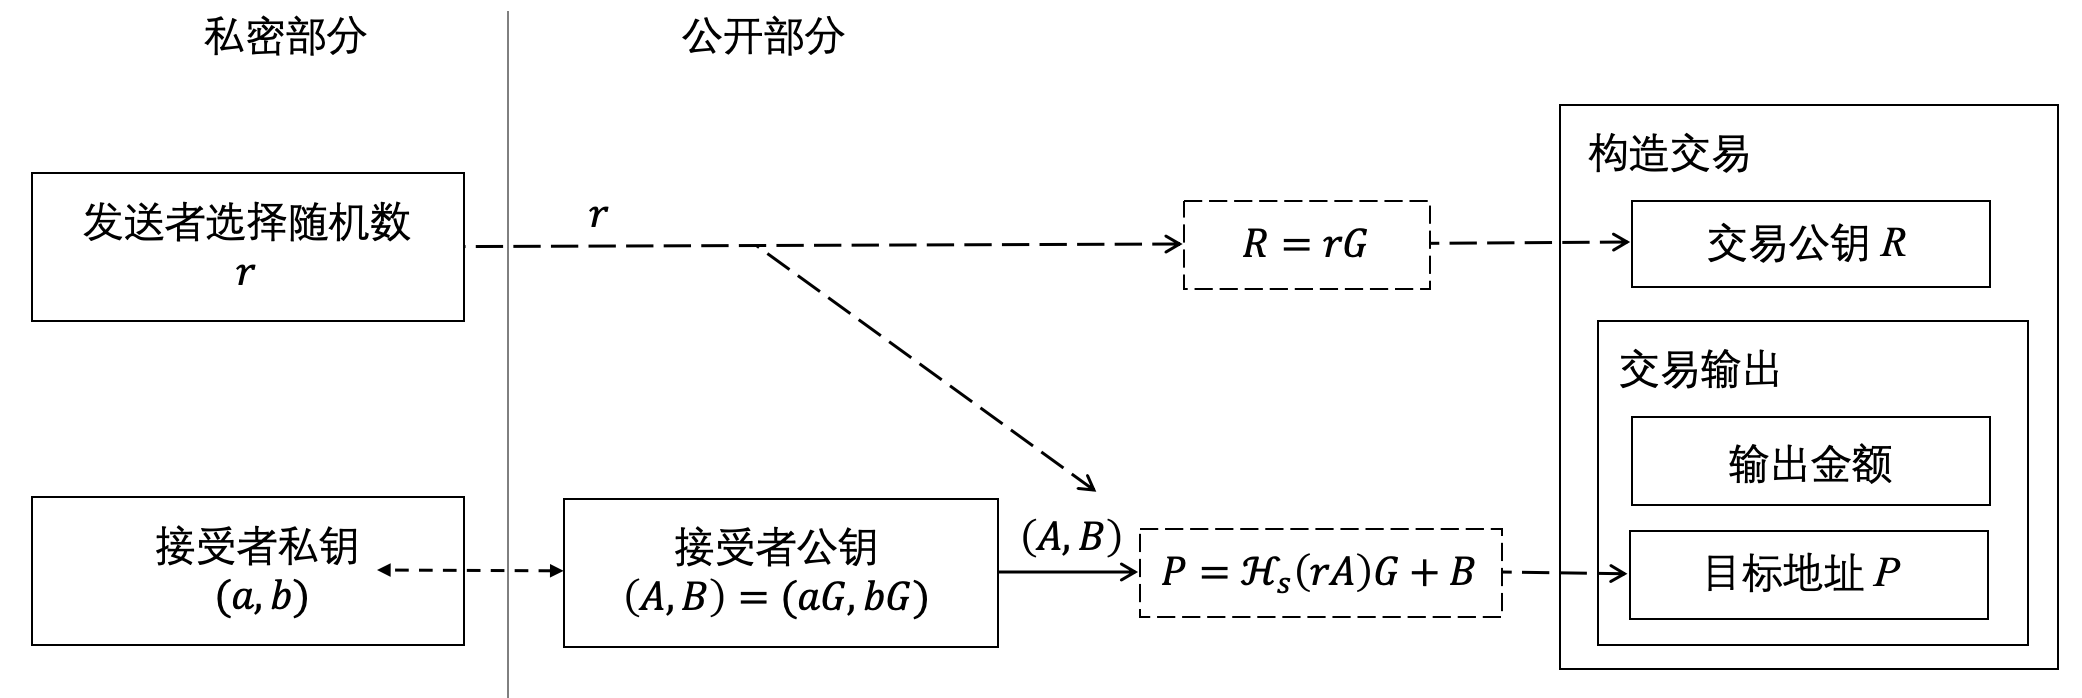
\includegraphics[width=7cm]{figures/one-time-gen.png}}%
  \hspace{4em}%
  \subcaptionbox{接受者生成一次性私钥,检查交易\label{fig:one-time-verify}}
  	{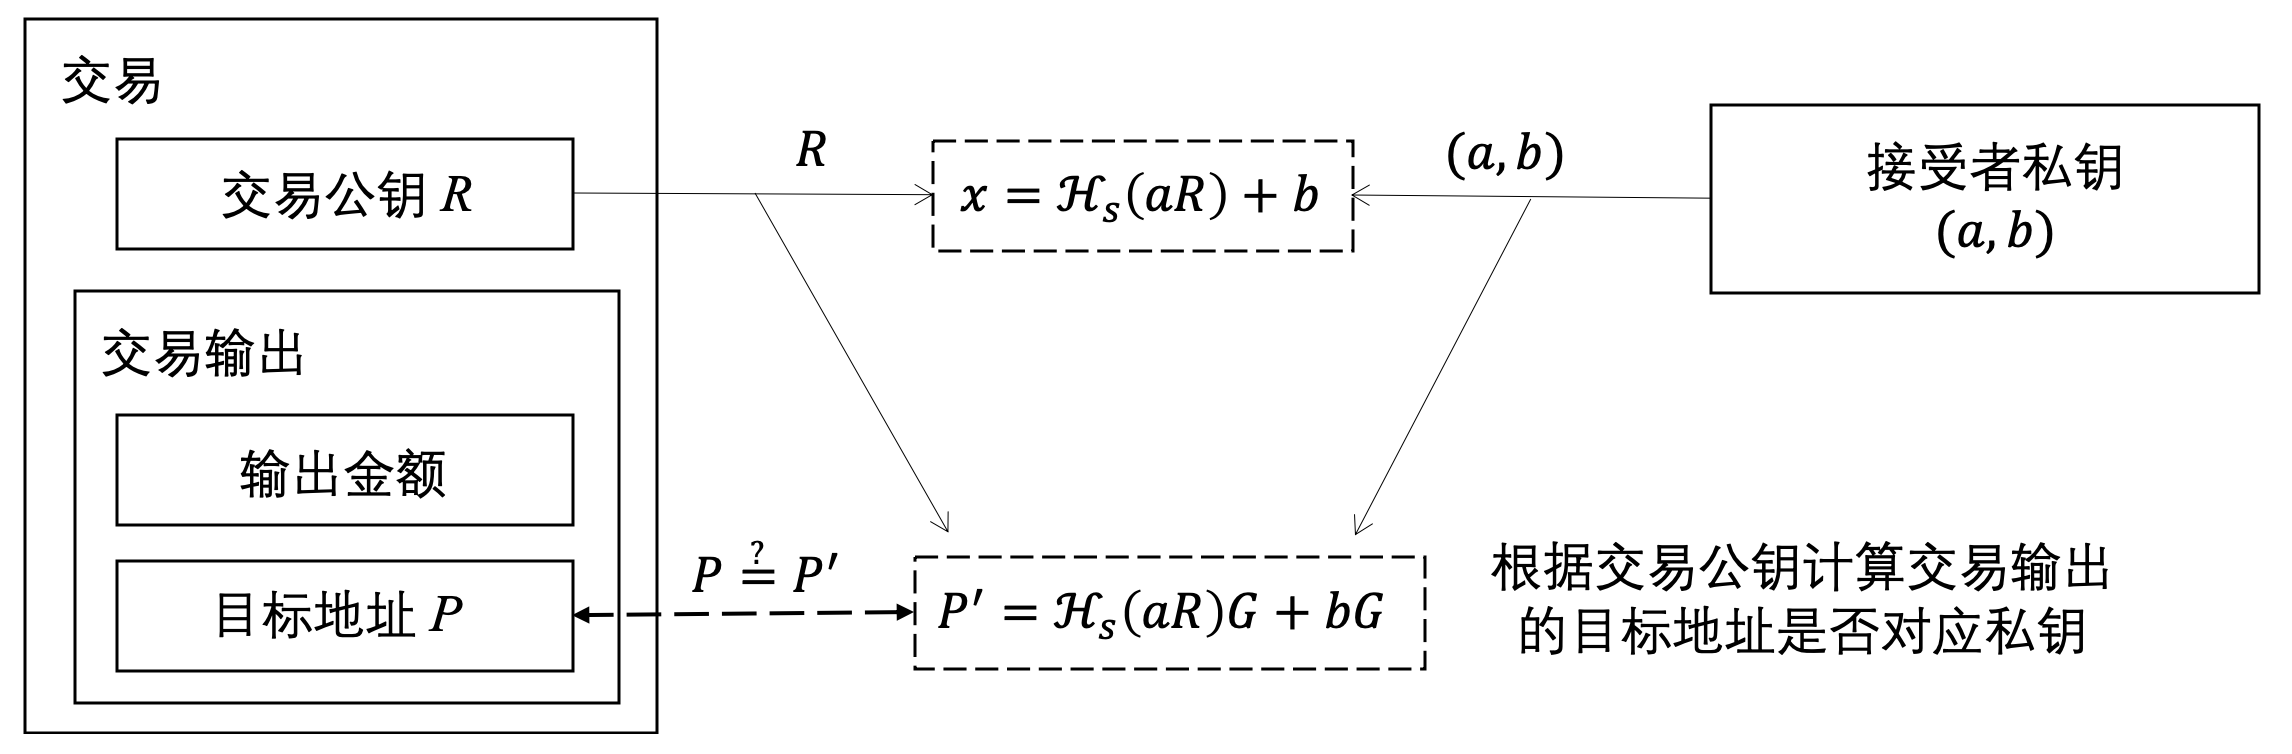
\includegraphics[width=7cm]{figures/one-time-verify.png}}
\caption{使用一次性公私钥对交易流程}
\label{fig:one-time-key}
\end{figure}

采用一次性公私钥对完成交易的流程如图\ref{fig:one-time-key},分为交易发起者生成交易与接受者检查交易两部分。交易发起者生成随机数与接受者公钥计算一次性公钥,作为交易的目标地址,并在交易中公布随机数对应的交易公钥。接受者用私钥与交易公钥计算一次性公钥判断是否为交易目标地址,如果匹配则能用私钥对该输出资产进行签名并花费。

为了满足不可追踪性,在发起交易的时候,CryptoNote协议改进可追踪环签名技术,在一次性公私钥对的基础上采用一次性环签名技术保护交易发送者隐私。一次性环签名同样分为生成签名与验证签名两阶段,并利用私钥哈希值作为快照保证资产对应私钥只进行过一次花费。

CryptoNote协议在交易中采用一次性公私钥对保护了接收方的隐私,采用一次性环签名保护了发送方的隐私。但CryptoNote协议采用环签名保护用户隐私的主要问题在于用户隐私依赖于选择的公钥集合,一旦集合中的其他用户公开使用了资产或发生隐私泄漏,导致输出被关联到对应地址,则该用户的地址关联情况也会被攻击者分析得出,导致隐私泄漏[56]。此后ByteCoin[57],Boolberry[58],DigitalNote[59]等一系列区块链项目都采用了CryptoNote作为底层框架来保护用户隐私。其中应用较为广泛的是Surae等人提出的Monero项目[60],该项目通过强制每笔环签名交易至少包含2个额外资产的方式,解决上述隐私泄漏的风险,增强了用户的长期匿名性[61]。

\subsubsection{机密交易技术}

2013年,Adam[62]提出引入同态加密技术[63]隐藏交易金额的思路,在不泄漏交易输入输出金额的具体数值的前提下,保障交易的输入输出资产金额相等。利用范围证明技术保障资产金额的数值在合法范围内,避免负数或越界的情况。2015年,Maxwell[64]对该想法进行了完善及实现,通过引入盲化因子避免了暴力枚举攻击,提出了机密交易技术(Confidential Transactions)。

机密交易技术中采用Pedersen承诺[65],在不透露交易金额的情况下使得其他节点能验证交易输入输出金额之和相等的正确性,利用椭圆曲线密码体系(ECC,Elliptic curve cryptography)[66]隐藏金额,并添加盲化因子保证在输入金额与输出金额相等的情况下,发起者才能对交易进行正确签名,同时盲化因子也能防止攻击者通过枚举暴力破解金额。为了防止负数和越界情况的出现,机密交易中采用环签名技术和盲化因子进行范围证明。但该方案采用的范围证明技术带来较大的时间复杂度和空间复杂度,为了解决这一问题,Maxwell提出一种新的环签名Borromean环签名[67]对该签名进行优化,可以提升到两倍的渐进效率。

然而,机密交易仅隐藏账本数据中的交易金额,不能隐藏交易发起者和接收者地址信息。2015年,Noether等人通过改进可链接自发匿名群签名(LSAG,Linkable Spontaneous Anonymous Group signature)技术[68],提出多层可链接自发匿名群签名(Multilayered LSAG)技术,并结合CryptoNote协议中的一次性环签名技术、一次性密钥对技术以及Maxwell提出的机密交易技术,提出了环机密交易技术[25]。该技术通过结合上述技术能同时隐藏区块链账本数据中交易金额、交易输入地址、交易输出地址。

\subsection{网络信息隐藏}

区块链系统的P2P网络中,攻击者通过部署足够多的节点监听网络中消息收发情况,可能将用户的IP地址与链上交易、地址等信息关联。因此除了对链上数据进行隔离的方法之外,为了保障区块链系统中用户IP地址的隐私,部分研究建议采用混淆网络对区块链系统进行加固,使得攻击者无法分析真正的消息发出方。现有的混淆网络主要基于两种路由技术:洋葱路由和大蒜路由,其中洋葱路由的代表项目为Tor网络,大蒜路由的代表项目为I2P网络。

\subsubsection{洋葱路由技术}

洋葱路由是一种保护网络通信的真实发送和接受节点,达成匿名通信的网络链路协议。洋葱路由通过对传输消息进行多层加密,使得路由中间节点只能知道前继节点和后继节点的IP地址,不能获取消息的真实发送节点IP与接收节点IP,保护消息发送方和接收方的真实IP不被攻击者知晓。除了出口节点外,其他中间节点也不知道消息的真实内容,保护消息内容隐私,因而只有出口节点知道自己属于出口节点,其他中间节点无法判断消息来源是客户端还是其他中转节点。

\begin{figure}
\centering
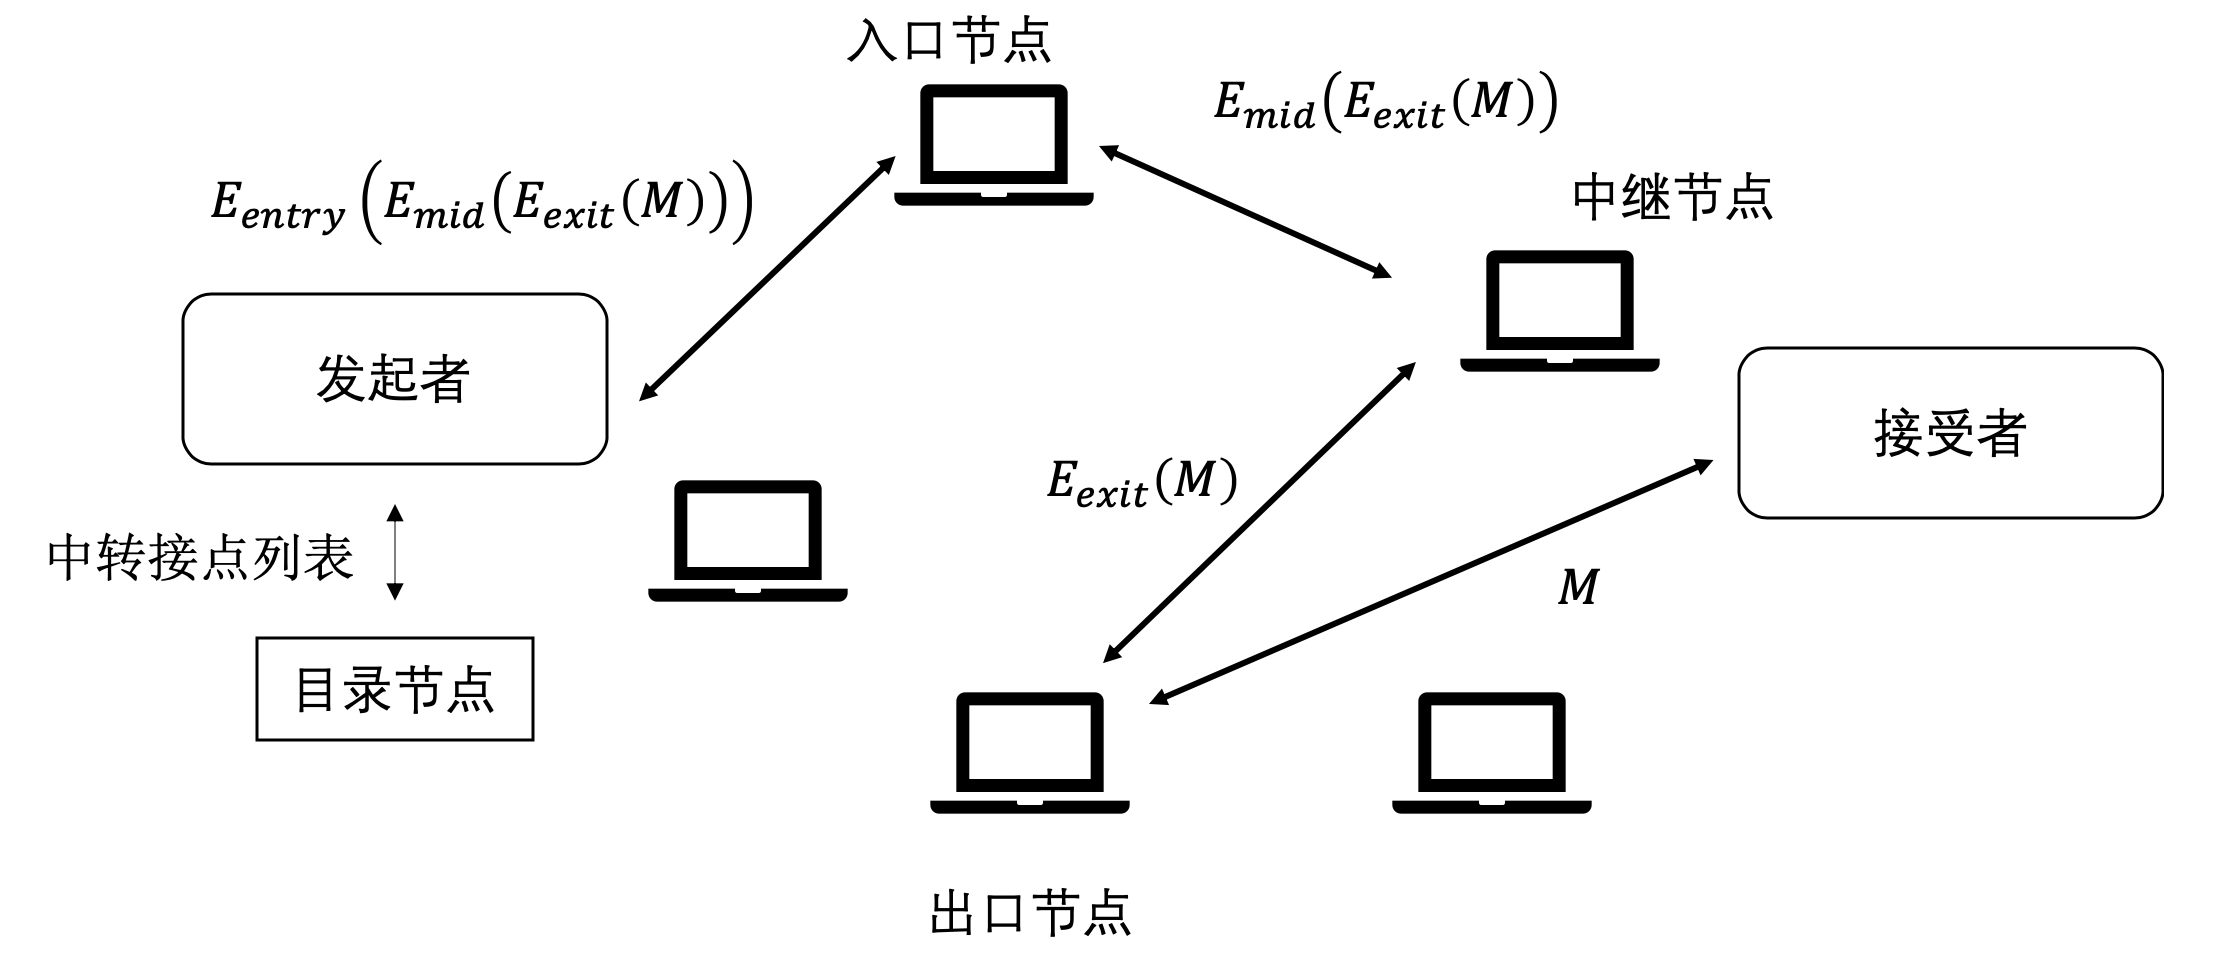
\includegraphics[width=10cm]{figures/tor.png}
\caption{Tor网络示例}
\label{fig:tor}
\end{figure}

基于洋葱路由原理的混淆网络项目主要有Tor网络[69],Tor网络建立发起者到接受者的链路主要包含以下三个阶段:

\begin{enumerate}
	\item 节点选择阶段:客户端从目录节点(directory node)提供的中转接点列表中随机选定网络中三个中转节点分别做为入口节点(Entry node)、中继节点(Middle Relay node)、出口节点(Exit Relay node)。
	\item 链路建立阶段:节点选择完成后,发起者从入口节点开始逐步建立链路。首先发起者与入口节点建立TLS链接,建立之后向入口节点发送信号,向中继节点建立链路,然后通过入口节点向中继节点发送信号,同样建立中继节点到出口节点的链路。
	\item 消息传输阶段:链路建立完成后,发起者可以通过该链路与接受者通信,所发送消息依次采用与三个中转节点协商好的会话密钥进行加密,中转节点层层解密,出口节点解密后发送给接受者。接受者返回信息沿原链路返回。
\end{enumerate}

为了增强用户隐私保护,部分比特币钱包内置了Tor网络配置,使得运行比特币钱包的节点可以通过Tor节点与比特币网络连接,从而保护节点的IP等隐私信息。采用Tor网络的比特币钱包可以在一定程度上抵抗网络监听攻击。但另一研究表明直接在Tor网络之上运行带黑名单机制的区块链项目(例如比特币)会带来安全隐患[70]。在比特币系统中,为了防止恶意节点进行拒绝服务攻击,节点设置了黑名单机制,当从某一节点接受到不合法消息后,会降低该节点信誉度,降低到0后加入黑名单,24小时内不接受该节点发送的消息。如果直接运行在Tor网络上,攻击者可以通过正常出口节点发送不合法消息给用户节点,迫使用户节点将所有正常出口节点加入黑名单,然后恶意节点通过部署自己的出口节点进行监听,这一攻击将威胁到用户身份隐私。

\subsubsection{洋葱路由技术}

尽管Tor网络采用洋葱路由技术保护通信匿名性,但是仍存在一定的安全隐患,例如流量分析攻击可以通过监听Tor网络中各节点的流量收发情况,分析网络中的流量变化情况,根据各Tor节点同一时刻的流量进出情况,判断节点间的链路关系,进而找出通信的真实发送方与接收方[71]。

为了抵抗流量分析攻击,大蒜路由将每个独立的消息称为一个蒜瓣,每个蒜瓣拥有对应的指示信息,表示该蒜瓣的类型和用途。客户端将多个蒜瓣封装成一个大蒜消息进行发送,拆分后通过不同链路传递,数据的返回采用不同的链路,同时数据往返采用的链路条数可以不同。因此基于大蒜路由的I2P网络(Invisible Internet Project)在抗流量分析攻击上比Tor网络更加安全。另一方面,I2P网络通过本地的Net DB发现节点,Net DB在每次链接其他节点时,采用Kad算法[72]进行更新,比Tor网络中的目录服务器方法有更强的安全性,但需要为此付出性能降低的代价。

\begin{figure}
\centering
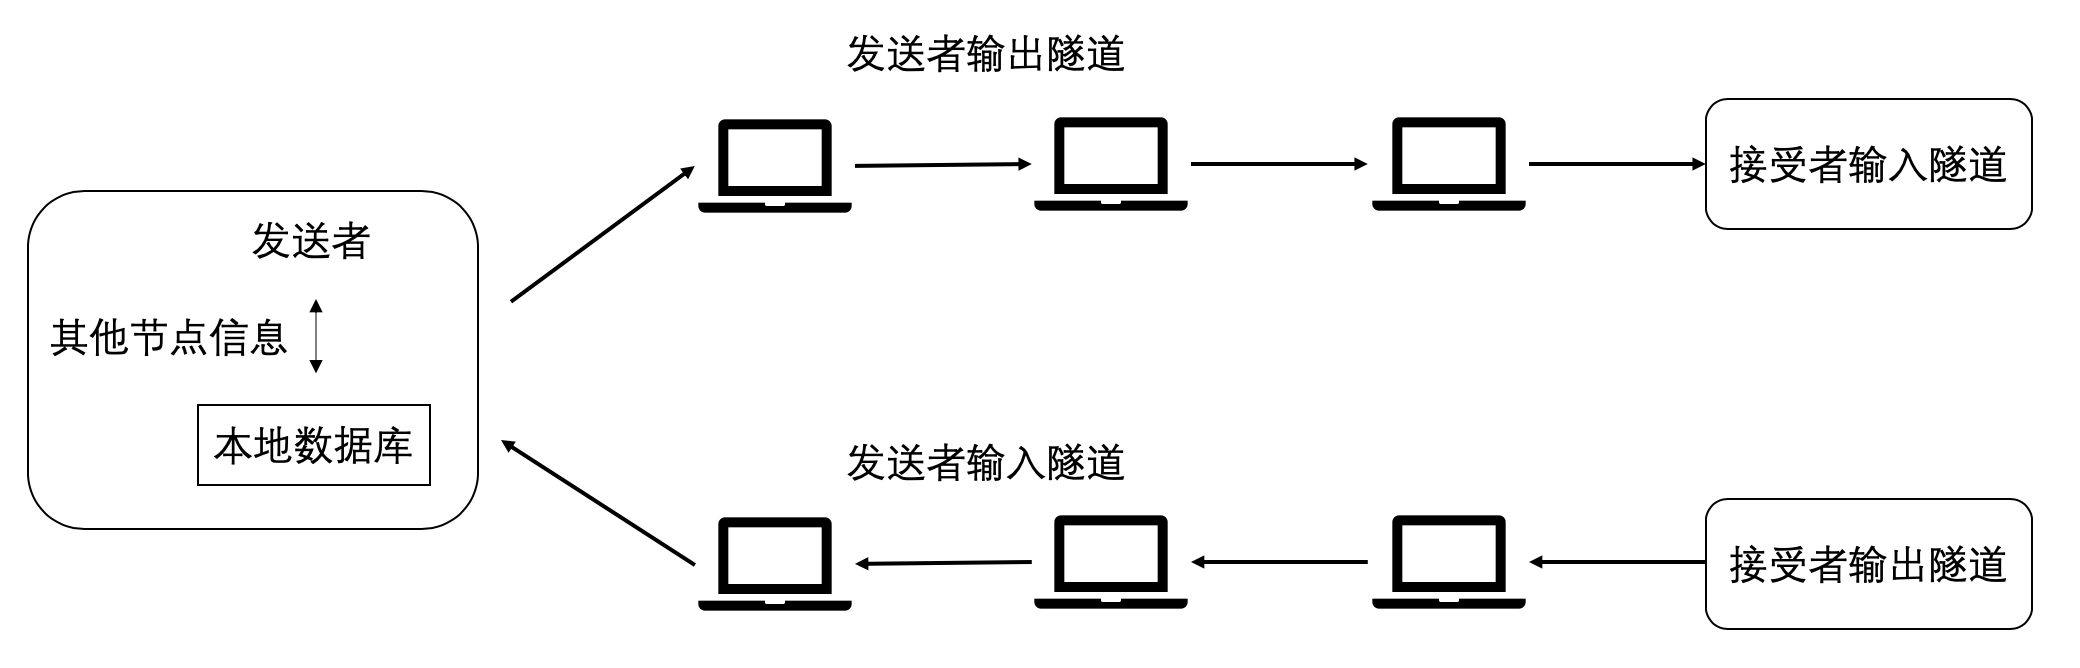
\includegraphics[width=10cm]{figures/i2p.png}
\caption{I2P网络中的隧道}
\label{fig:i2p}
\end{figure}

I2P网络中,用户通过传递可变隧道建立(VTB,Variable Tunnel Build)消息建立输入输出隧道,每个VTB消息由多个建立请求记录(BRR,Build Request Record)组成,其中每个BRR包含接受节点信息和其他相关信息。I2P网络建立隧道与Tor网络同样采用多层加密技术,但在发送消息和返回消息采用输出和输入两条不同链路,使得流量保持单向传输,通信双方的输入输出隧道将构成环路,能隐藏真实的通信节点,抵抗流量分析攻击。I2P网络通过分离链路的方式进一步隐藏了隐藏网络中流量情况,在Tor网络的基础上进一步增强了用户隐私安全。

\section{通道隔离机制}

通道隔离机制从网络层面对数据进行隔离,保护数据只对通道内节点可见。通过对账本进行隔离,每个节点只处理并存储自己所在通道的数据,防止攻击者访问数据,保护用户隐私。但是通道机制也存在一定缺陷,主要体现在区块链网络中通道部署存在一定代价,节点创建和进出通道需要进行网络配置的修改,灵活性较弱。根据被隔离数据的存放位置,通道隔离机制的实现技术可以分为链下通道隔离和多链通道隔离两大类。

链下通道隔离主要应用于高频小额交易,用户通过在区块链上记录起始的状态创建通道,随后在链下进行交易,具体数据通过合约保证安全,但不公布记录在区块链上,需要中止交易的时候再将最新的结束状态公布并记录在区块链上,终止通道并销毁历史交易记录。

多链通道隔离通过在特定节点之间构建独立通信网络作为通道,该网络中信息单独存放在子账本中,非通道内节点不能访问,同一节点可以加入多条不同通道中。多链通道隔离通过在网络层面构建子网络,实现节点通信隔离,杜绝攻击者访问隐私信息,保护用户隐私。

\subsection{链下通道隔离}

为了解决区块链账本容量有限的问题,研究者尝试将小额高频交易放在链下的微支付通道进行,仅仅将通道启动和结束的信息记录在区块链账本上。典型的微支付通道技术为比特币系统中的闪电网络技术[26]与以太坊系统中的雷电网络技术[27]。其中闪电网络技术针对基于未花费交易输出模型的密码货币,雷电网络主要针对基于账户余额状态模型的密码货币,更多利用链上合约机制。该技术主要分为两步,首先在两个节点之间构造链下双方支付通道,然后通过节点间的双方支付通道构建支付网络。

双方支付通道:在两个地址间构建可信的链下支付通道。通过将资产托管到链上合约创建支付通道,随后参与双方通过对状态更新进行签名确认进行交易,具体过程不需要记录到区块链账本中。当某一方希望中断通道时,将最新状态发布到区块链中,并赎回最新状态对应资产。
构建支付网络:在所有参与用户之间两两构建双方支付通道会带来巨大的存储资源和资产的浪费。因此在双方支付通道的基础上,用户通过已有的双方支付通道进行支付,从而构建全体用户之间的支付网络。

\subsubsection{闪电网络技术}

2016年,Poon等人提出了比特币系统中的闪电网络技术[26],该技术主要由序列到期可撤销合约(RSMC,Revocable Sequence Maturity Contract)和哈希时间锁定合约(HTLC,Hashed Timelock Contract)组成,利用RSMC实现双方支付通道,通过HTLC进一步构建支付网络。这一设计在提高比特币系统性能的同时,也通过隐藏不在链上记录用户间的小额支付保护了用户隐私。

\begin{figure}
\centering
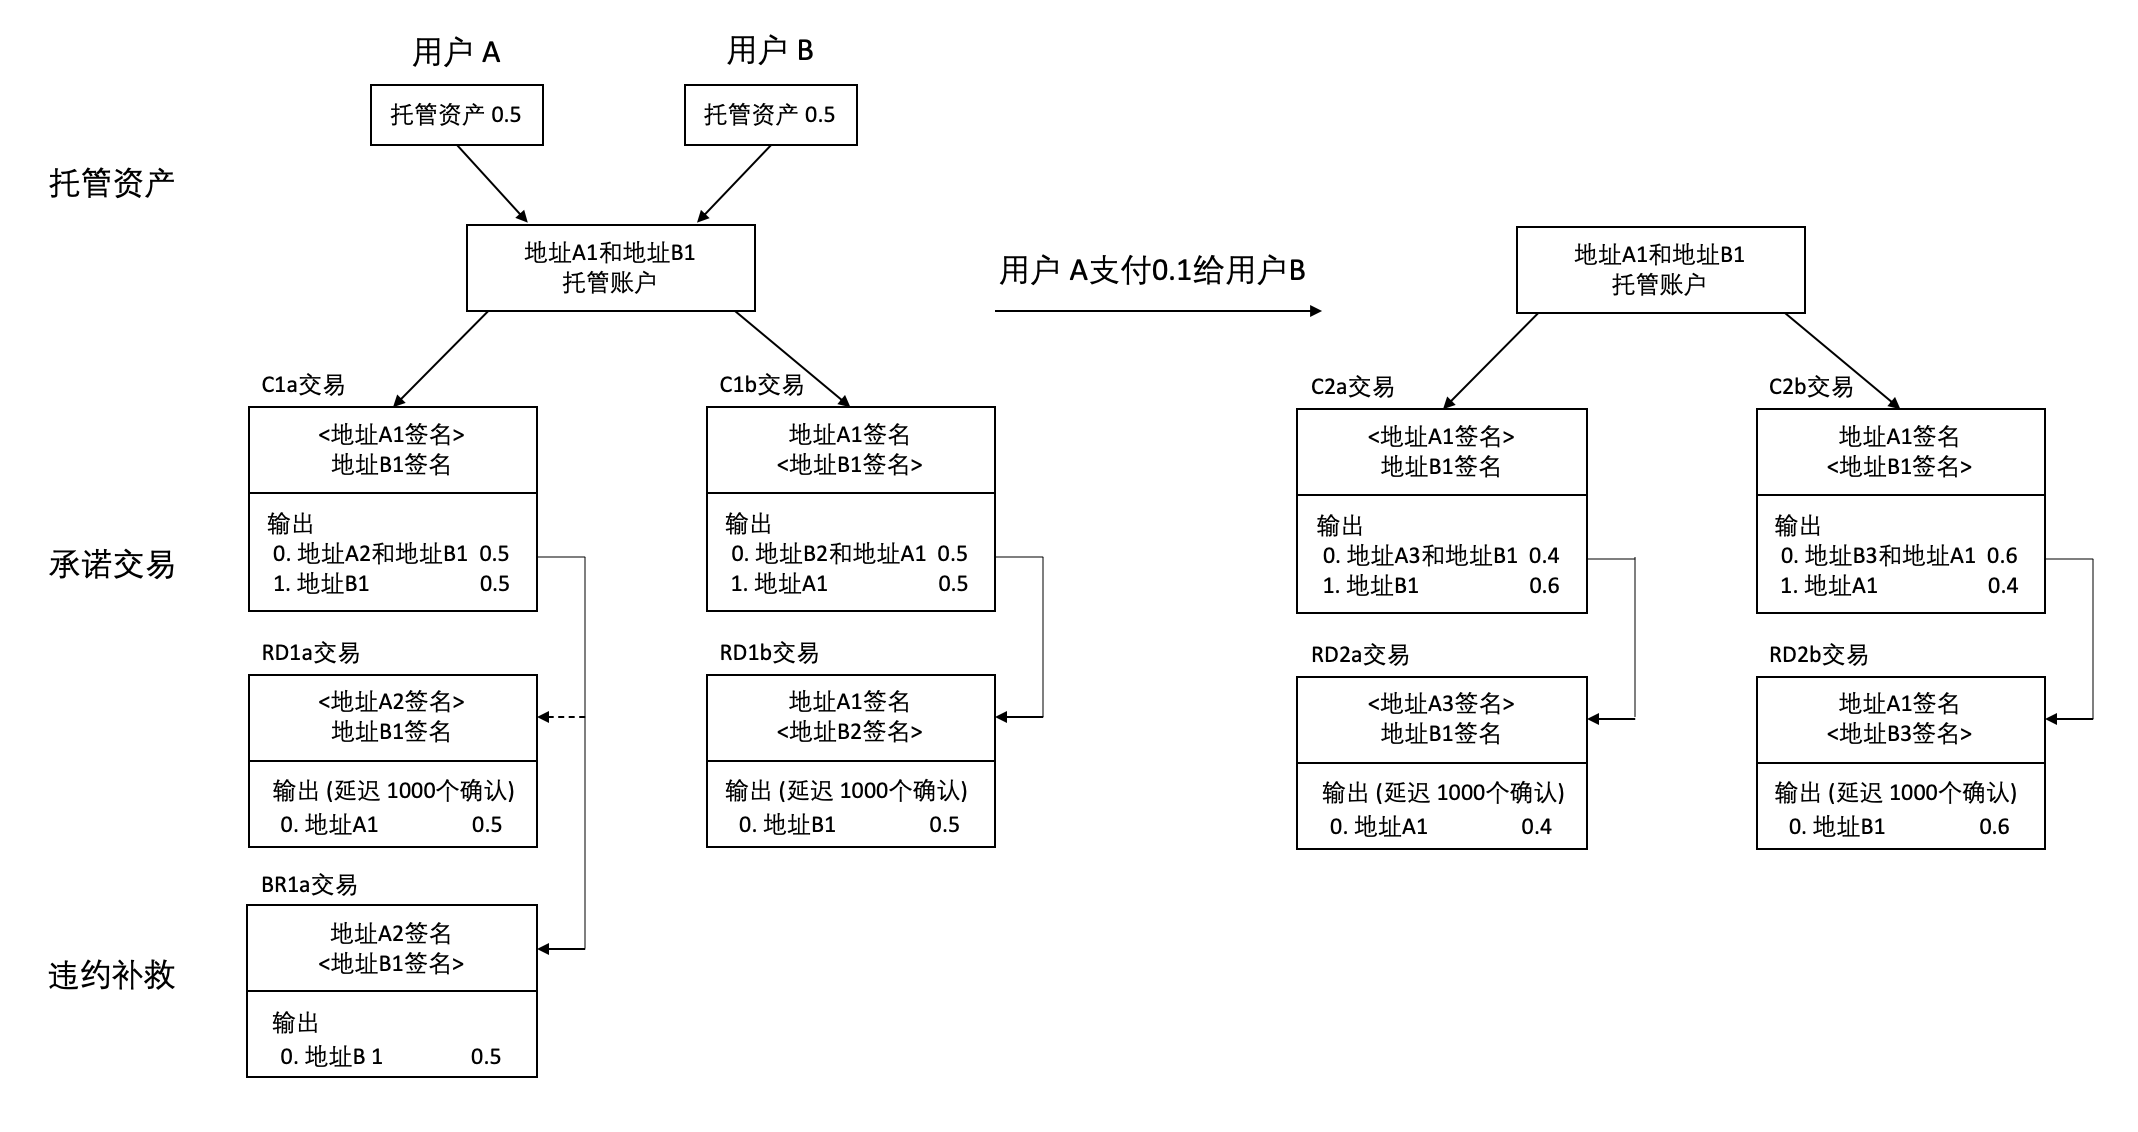
\includegraphics[width=10cm]{figures/lightning-network.png}
\caption{序列到期可撤销合约的通道创建和状态更新}
\label{fig:lightning-network}
\end{figure}

双方支付通道: 序列到期可撤销合约(RSMC)通过不断创建2/2多重签名钱包,构建双向支付通道。只在合约创建和结束时各在比特币账本上发布一次的特性,保障用户隐私。图17展示了一个具体的序列到期可撤销合约的创建及支付过程:

\begin{enumerate}
	\item 托管资产阶段:用户A和用户B双方各拿出部分资产,托管到双方签名账户,该账户的支出需要双方共同签名,此后支付阶段中支付通道的交易状态各用户花费不能超出所托管资产。但双方不对托管交易签名,更不广播到区块链网络。
	\item 构造通道阶段:用户A构造承诺交易1a(C1a,Commitment transaction 1a)和可撤销支付交易1a(RD 1a,Revocable Delivery 1a),并交给用户B签名。C1a交易用于保证在用户A单方中止通道的情况下,Bob能得到自己的托管资产。RD1a用于保证用户A能单方取回自己托管的资产,该交易带有延迟设定,若C1a被记录在第n个区块,则RD1a只能记录在第n+1000个区块之后的区块。Bob对称构造承诺交易C1b和RD1b,并交给Alice签名。双方均完成对承诺交易和可撤销支付交易的签名并交换后,各自再对托管交易进行签名并广播,合约建立完成。
	\item 支付阶段:当用户A支付0。1单位资产给用户B时,首先需要将C1a和RD1a代表的状态作废,用户A构造并签名违约补救交易(BR1a, Breach Remedy 1a),发送给用户B,因此当用户A发布C1a后,在1000个区块时间内,用户B可以发布BR1a。然后双方按照构造通道阶段中的步骤,根据支付后的余额分配情况重新构造承诺交易C2a、C2b以及可撤销支付交易RD2a、RD2b,完成状态改变。
	\item 结束阶段:当任一方用户希望结束合约时,先公布承诺交易,若另一用户未在延迟时间中公布违约补救交易,则表示该承诺交易为最终状态,该用户在延迟时间后再公布可撤销支付交易取回资产。
\end{enumerate}

\begin{figure}
\centering
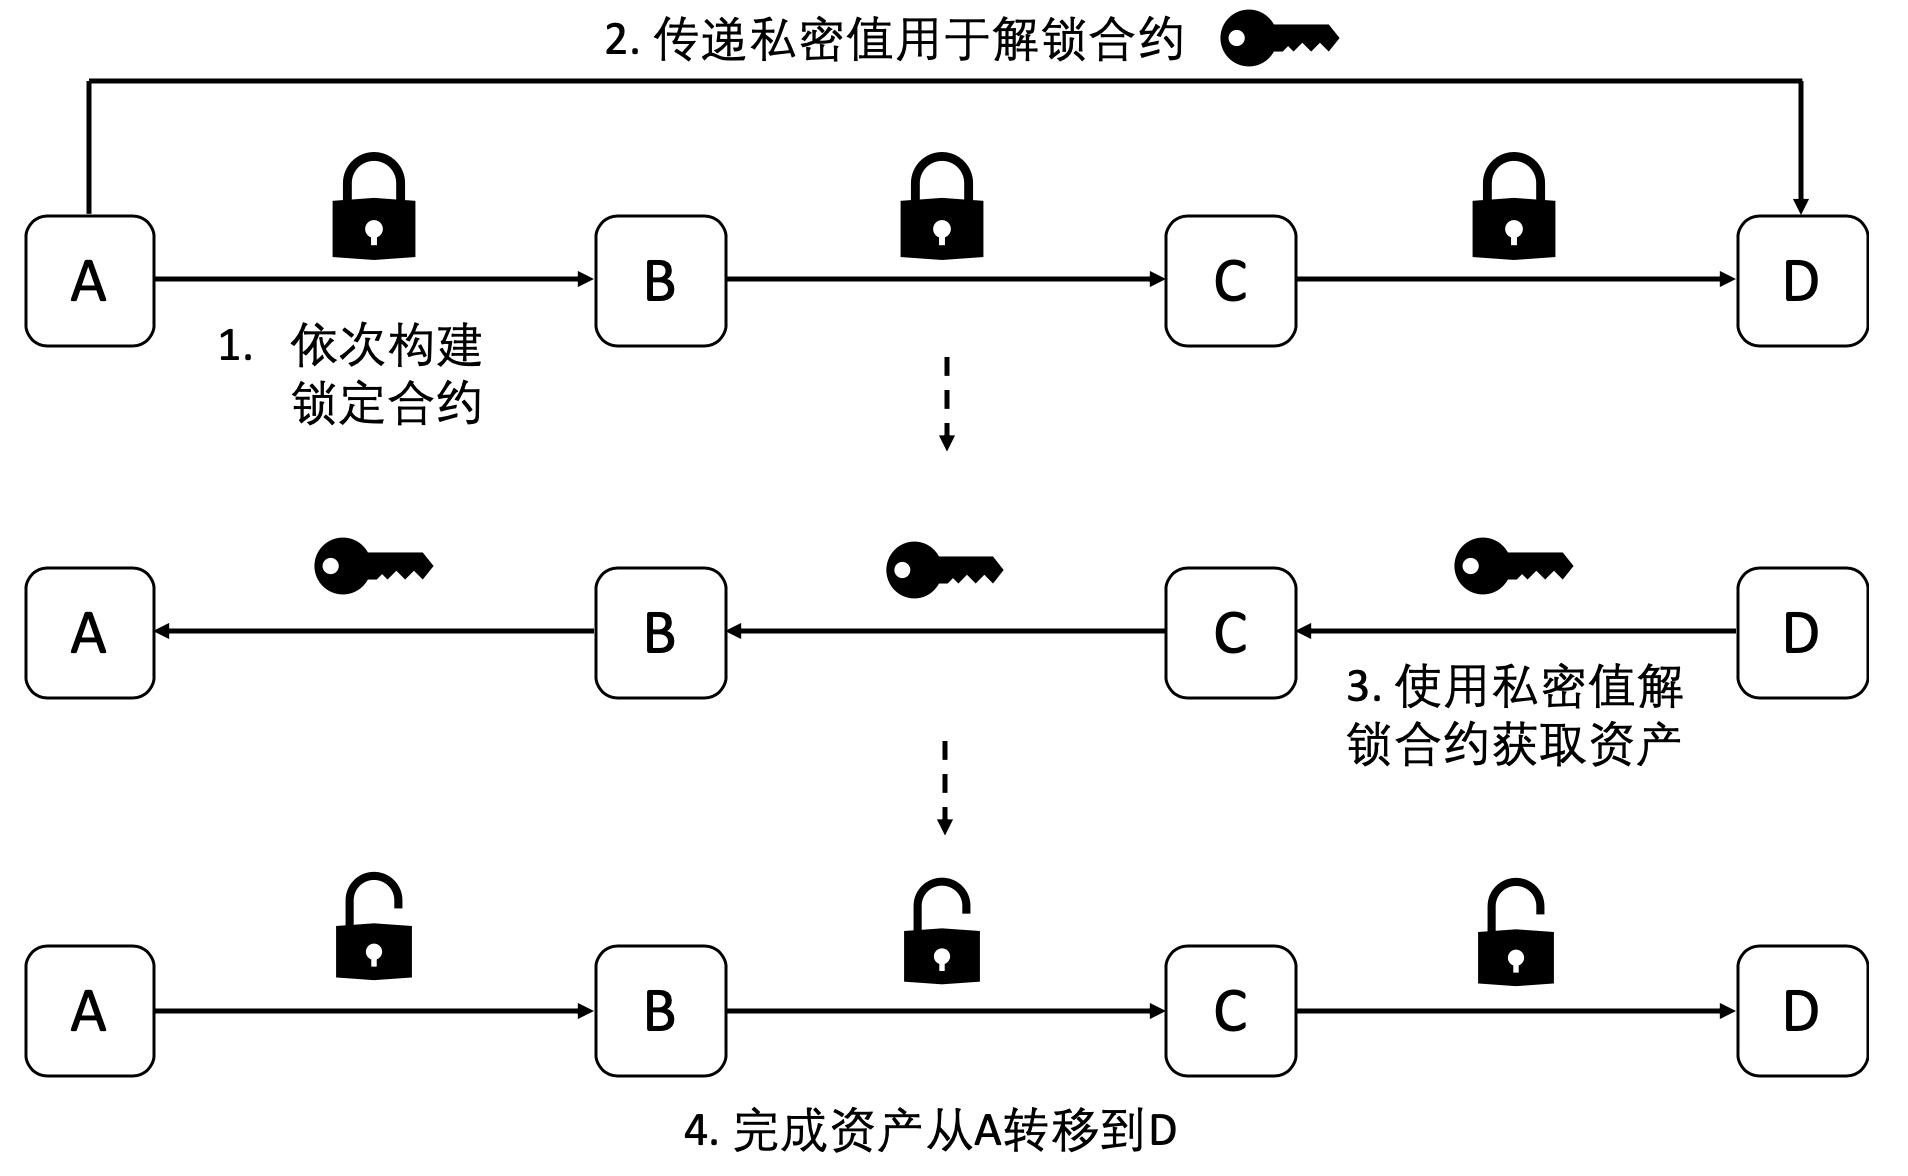
\includegraphics[width=10cm]{figures/hash-time-lock.png}
\caption{哈希时间锁合约的工作流程}
\label{fig:hash-time-lock}
\end{figure}

构建支付网络:哈希时间锁定合约(HTLC)是一类特殊的链上合约交易,通过哈希时间锁构造的链上合约保障交易双方能通过中间人进行安全交易,利用哈希原象作为支付凭证,三方参与的哈希时间锁定合约具体细节已在2。2。2节中详细介绍。多人采用哈希时间锁定合约可以帮助未建立RSMC的两个用户通过中间人建立交易通道。如图\ref{fig:hash-time-lock}所示,在AB、BC、CD之间分别存在RSMC时,AD之间可以通过已有通道完成支付。
闪电网络技术通过RSMC保障链下支付通道的资产安全性,通过HTLC减少网络中所需RSMC的数量,增强闪电网络的扩展性。利用闪电网络技术,用户之间往来的交易数据将不会记录在区块链账本上,杜绝了账本分析攻击,极大保障了用户的账本隐私安全。

\subsubsection{雷电网络技术}

在闪电网络技术的基础上,雷电网络技术[27]基于以太坊系统的智能合约机制提供更加便捷的链下支付通道。雷电网络同样分为构建双方支付通道和多方支付网络两部分,利用图灵完备的智能合约语言,简化了闪电网络中序列到期可撤销合约(RSMC)和哈希时间锁定合约(HTLC)的实现方式。

双方支付通道:雷电网络中的支付通道主要分为合约构建、余额证明、链下支付、合约撤销几个阶段。合约构建阶段由参与者为特定通道创建智能合约并发布到区块链账本。余额证明阶段中,通道中的交易双方通过向合约账户进行转账作为资产抵押,此后通道中的交易额度不可以超过证明的资产数量,保证交易双方有偿还债务的能力。完成证明后,链下支付阶段中,交易双方根据合约规定的格式,通过对更新的交易状态签署新的余额证明完成链下支付,每一次状态消息都附加上递增的序列号。闪电网络中每次记录的是新的余额状态,而雷电网络中记录的是更新的资产变化。当某一方希望中断支付通道时,停止签名新的状态消息,将当前的状态消息发送给智能合约。在一定时间内,如果合约未收到序列号更大的状态消息,则进行合约撤销,根据最新接受的状态消息返回资产到各参与者账户。

\begin{figure}
\centering
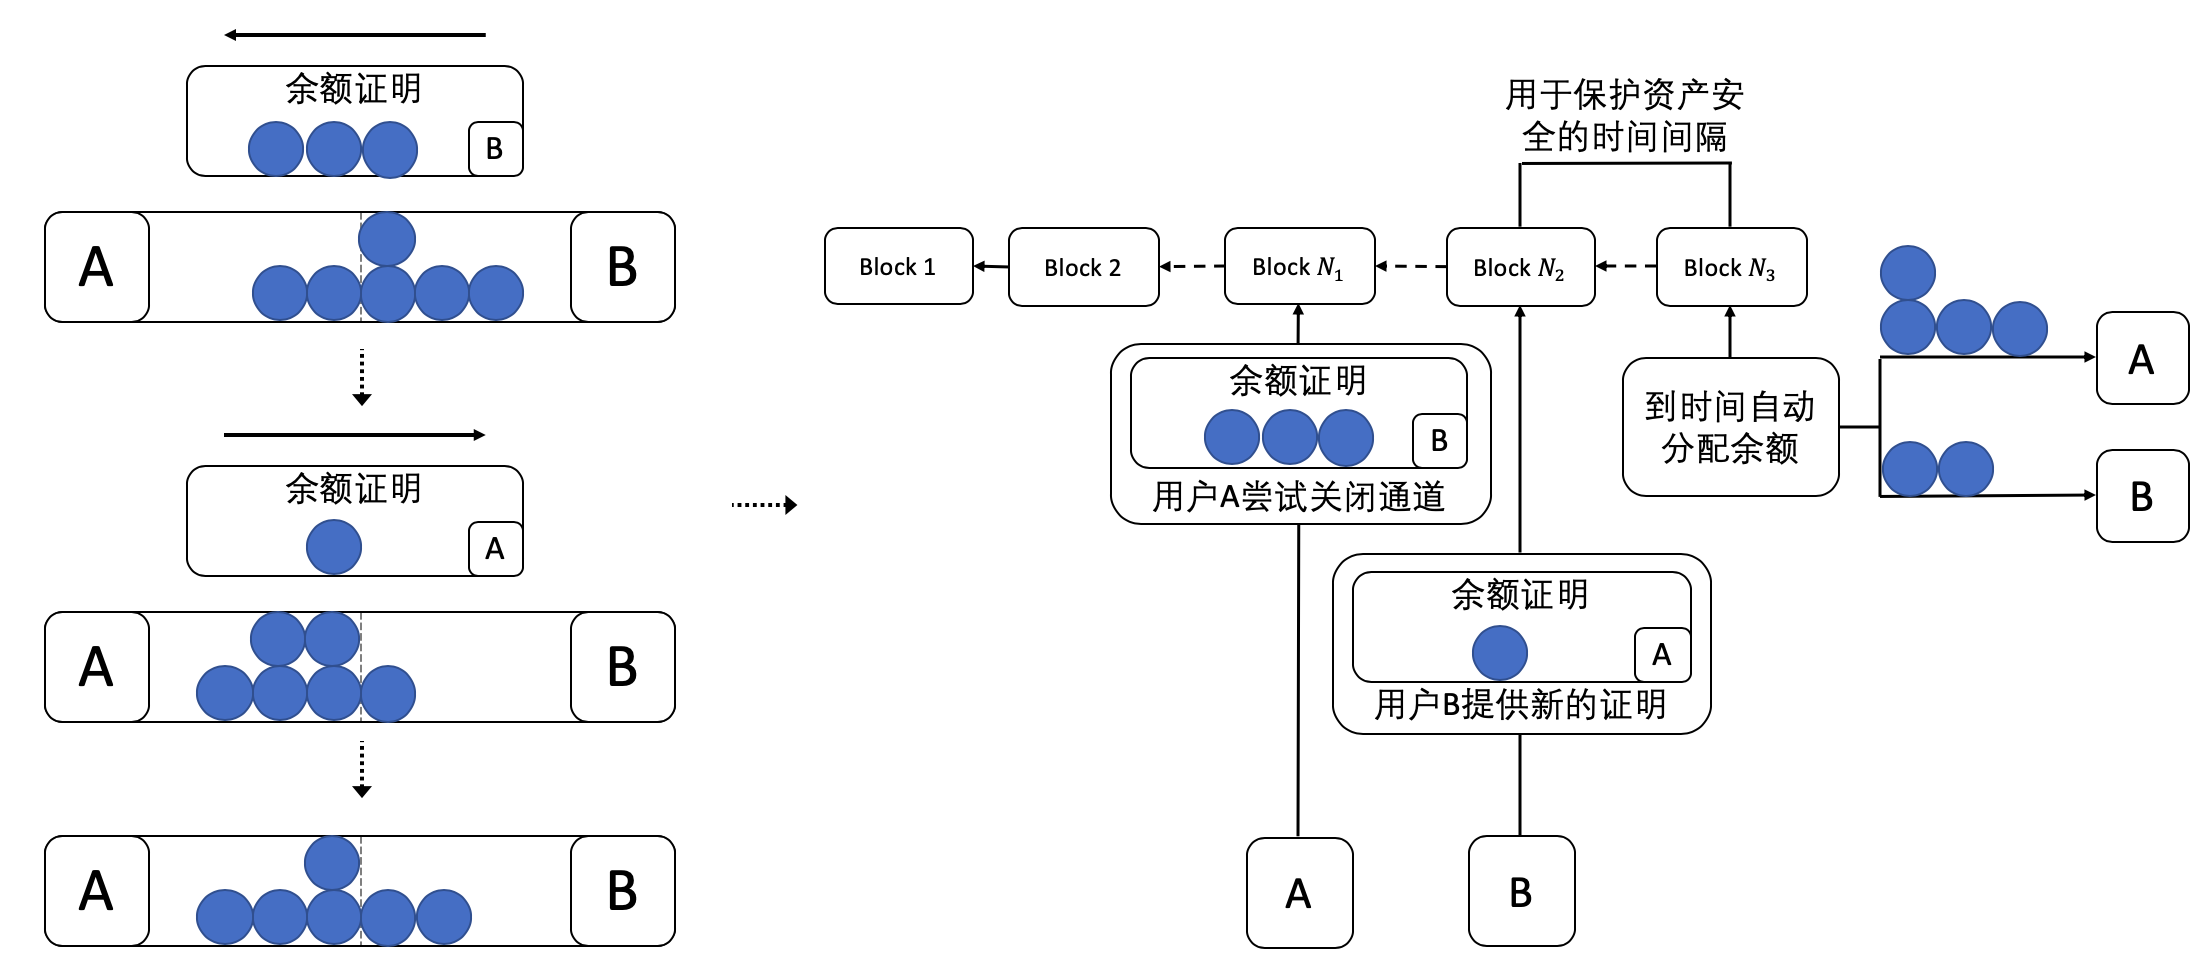
\includegraphics[width=10cm]{figures/raiden-channel.png}
\caption{雷电网络技术的支付通道示例}
\label{fig:raiden-channel}
\end{figure}

如图\ref{fig:raiden-channel}所示,第一步用户B向用户A先支付3个币,第二步用户A向用户B支付1个币。之后用户A尝试使用第一步的余额证明关闭通道,在限定时间内用户B提供新的余额证明,保证最终余额分配是按照最新状态进行。

多方支付通道:由于闪电网络技术中的HTLC存在中间用户与收款用户合谋损害付款用户资产安全性的风险,例如当用户A通过中间用户C向用户B进行支付,用户A发布向用户C支付的锁定合约后,用户C假装离线,用户A重新选择中间用户D完成支付。此时若仍在AC之间合约有效期内,用户B可以提供私密值使得用户C获取合约AC锁定的资产。为了解决这一问题,雷电网络技术在收据哈希锁(receipt hash lock)和时间锁(time hash lock)之外增加重试哈希锁(retry hash lock),该锁用于中间用户离线导致付款人需要改变支付路径的情况。雷电网络技术中的三方支付通道过程中同样由收款用户创建哈希锁并保留哈希原像作为解锁私密值。付款用户构造重试哈希锁同样保留哈希原像,并使用收到的收据哈希锁和重试哈希锁构造支付交易。等待中间用户正确发布支付后再将重试哈希锁的私密值发送给收款用户用于获取资产。若中间用户离线需要更换支付路径,则将旧交易作废,重新构造重试哈希锁,保障付款用户资产安全。

\subsection{多链通道隔离}

多链通道隔离技术在同一区块链系统中维护多个区块链账本,其中不同节点群体维护特定子区块链,通过设置访问控制机制保障子区块链数据隐私安全。

目前较为成熟的多链通道技术主要为HyperLedger Fabric项目[4]中的通道技术,通道技术主要通过在不同团队的内部节点间分别独立构建区块链,保护内部数据的隐私安全。分片技术将同一区块链账本拆分为多个分片进行维护,各分片只负责维护不同的账户信息以及事务数据,不需要验证全局的账本信息。在必要情况下分片之间需要进行通信。多通道技术在不同节点间构建互相隔离的通道,维护各自的独立账本,不同通道之间不需要进行通信,因此更强地保护用户隐私数据。

在实际的应用场景中,不同节点具有不同的链下身份,需要完成不同的业务需求,因而会根据业务组成不同的团队进行合作。为了保护同一团队内部节点间的隐私数据,多通道技术通过在不同团队的内部节点间分别独立构建区块链,维护账本数据,保护内部数据的隐私安全。多通道技术主要包含以下机制:

\begin{itemize}
	\item 身份管理:管理各节点身份授权及认证机制,持有不同身份的节点拥有相应权限。
	\item 通道管理:管理通道建立、维护、销毁的整个生命周期。
	\item 事务管理:管理通道内事务的发布、排序、记录等操作。
\end{itemize}

\begin{figure}
\centering
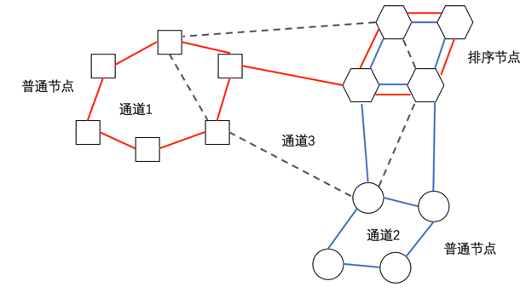
\includegraphics[width=10cm]{figures/hyper-channel.png}
\caption{超级账本通道机制}
\label{fig:hyper-channel}
\end{figure}

2017年,HyperLedger Fabric项目更新1.0版本并增加了通道机制。网络中的若干节点可以通过网络配置搭建通道,在同一通道中的节点共同维护子账本数据,通道中传输的数据不被通道外的用户接收。而某一节点可以根据自己的实际需求加入多个通道,实现了商业场景下的不同业务数据隔离。

综上所述,通道隔离技术在网络层面进行消息隔离,通过限制消息的传播范围保护用户隐私。在非许可链系统中,区块链账本对所有节点公开,因此通道主要以链下通道的形式存在,用户通过构建链下通道保护账本数据隐私,同时利用公有链账本记录通道的开启和结束保护交易安全。而在许可链系统中,主要采用传统的授权与认证技术,由于存在访问权限的设计与管理,网络配置有了更多的选择,通常采用多链机制,根据应用需要构建不同的子区块链。

\section{小结}

随着区块链技术的成熟与众多区块链系统的广泛使用,以及未来区块链技术将在更多的领域中发挥作用,区块链系统中的用户隐私威胁将会成为更加重要的研究问题。本章将现有的隐私保护技术归纳总结为地址混淆、信息隐藏、通道隔离三类机制,并详细介绍了各类隐私保护机制的原理、特征以及不同的实现方式。现有的各类隐私保护机制及实现技术从不同方面保护区块链隐私,但存在安全性、性能、扩展性等方面的不足。

% !TeX root = ../main.tex

\chapter{BACS系统中的隐私保护}
\label{chap:privacy-design}

在第\ref{chap:bacs}中,我们介绍了基于区块链技术的ABAC访问控制系统。这一系统能增强现有访问控制系统的安全性,但引入联盟网络对用户信息进行共同管理,会导致联盟网络中任何节点都可以查看用户在系统中进行的授权信息和历史状态,带来用户隐私泄漏的风险。

第\ref{chap:privacy-survey}章对现有的隐私保护技术进行总结归纳。其中,zk-SNARK技术的优点在于生成的证明大小和验证证明的时间花销都是常数大小,缺点在于需要可信的初始化密码参数。因此,这一技术并不适用于公有链系统。而在BACS系统中,联盟链网络中节点可以通过安全多方计算技术共同参与密码参数的初始化过程,保障系统安全可信。同时,zk-SNARK技术提供常数级复杂度的验证可以保障BACS系统的实时性。

本章首先简要介绍zk-SNARK技术中的R1CS约束,QAP问题,同态加密三个主要步骤,然后介绍结合ABAC访问控制系统,区块链上授权的数据结构以及运用zk-SNARK技术进行隐私保护的方法。

\section{zk-SNARK技术}
\label{sec:zk-SNARK}

简明非交互式零知识证明(zk-SNARK,zero-knowledge Succinct Non-interactive ARguments of Knowledge)技术在非交互式零知识证明证明技术的基础之上进行优化,保持非交互性的同时,减少了证明大小,节省存储空间与验证时间。由于最终生成的证明转化为固定大小的多项式抽样验证,该技术的优点在于生成的证明大小为常数,验证该证明的时间花费也是常数。因此该技术能应用于区块链系统中事务合法性的证明和验证。缺点在于该技术需要可信的启动过程,通过一系列密码学参数来生成加密密钥和验证密钥,掌握这一类系列密码学参数即可伪造证明。该技术主要包含以下3个步骤:

\subsection{R1CS约束}

先将计算拆分为一阶线性约束等式(R1CS, Rank-1 Constraint System),这一过程类似编译器对高级语言程序进行处理到中间表示,每一步计算被转换为
$$s \cdot a * s \cdot b - s \cdot c == 0$$整个函数可能包含数百条甚至更多的R1CS约束,为了简化表示,也为了后面进一步简化,可以用矩阵的形式表达为
$$s \cdot A * s \cdot B - s \cdot C == 0$$

\subsection{QAP问题}

由于R1CS得到的矩阵形式中,每个矩阵包含若干列,对于每一行,可以通过拉格朗日插值公式构造特定函数fi(x)使得当x取值0到n的时候,刚好fi(x)值对应第i行第x列的数值。矩阵形式转换为多项式形式。

$$s \cdot A(x) * s \cdot B(x) - s \cdot C(x) == 0, \forall x = 1, ... , n$$

令$Z(x) = (x-1)(x-2)...(x-n)$,由多项式零点的性质可得s \cdot A(x) * s \cdot B(x) - s \cdot C(x)被$Z(x)$整除,即
$$s \cdot A(x) * s \cdot B(x) - s \cdot C(x) == Z(x)*H(x)$$ 对任意$x$成立

因此我们只需要验证该多项式等式是否即可,但由于多项式参数个数与约束数量相等,目前的验证未能节省时间。为了简化验证复杂度,因为该多项式在任意点都成立,因此通过验证一个特殊点,能以较大概率验证该多项式是否为0。因为2n次的多项式最多有2n个零点,证明者在不知道该特殊点的情况下伪造证明的概率约等于0。

\subsection{同态加密}

将计算的验证转换为对多项式等式的验证,并通过对点的抽样计算完成对整个多项式等式正确性的检验。基于椭圆曲线的双线性对性质隐藏用于计算的真实输入,包括证明者给定的隐私输入,以及验证者使用的特殊点。利用可信创始方初始化阶段生成的参数实现零知识证明.这一过程利用同态加密的加法同态性以及椭圆曲线的双线性对函数。验证者首先对特殊点t,生成t的次方加密后的值如下
$$E(1),E(t), E(t^2), E(t^3),..., E(t^n)$$

证明者可以通过这一系列参数计算出$E(A(t)),E(B(t)),E(C(t)),E(H(t))$。验证者为了验证$A(t)*B(t)-C(t) = Z(t)*H(t)$成立,只需要验证$E(A(t))*E(B(t))-E(C(t)) = E(Z(t))*E(H(t))$成立即可。这一证明可以隐藏证明者的特定输入$s$。

在访问控制系统中,存在资源服务器作为可信的启动方,独立生成初始密码学参数,不用担心其他人获取这些参数伪造证明。用户只需要根据资源服务器提供的加密密钥,以及自己的账户信息生成凭证,该凭证隐藏用户状态等部分敏感输入信息。资源服务器通过验证该凭证即可判断用户是否有权限执行提交的操作申请,并进行正确回应。具体设计将在第二部分介绍。

\section{BACS系统中的隐私保护设计}

在第\ref{chap:bacs}章中,我们提出了基于区块链技术的访问控制系统BACS,该系统中的授权数据结构和访问请求数据结构如图\ref{fig:data-structure}所示。其中,关键隐私信息为相关地址、授权属性、操作对象、操作类型等。该方案采用私钥签名作为来源凭证,在提供身份证明的同时暴露用户隐私信息。因此,本节将介绍采用zk-SNARK技术隐藏授权和访问中的关键信息。

\begin{figure}[ht]
  \centering%
  \subcaptionbox{授权信息数据结构\label{fig:auth-data}}
    {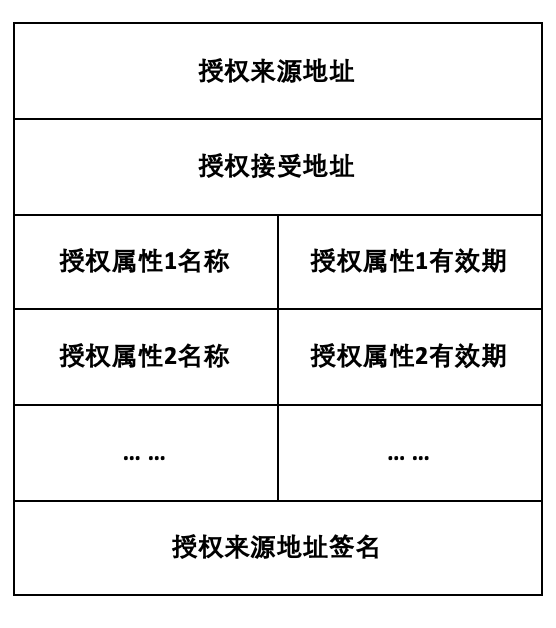
\includegraphics[width=6cm]{figures/auth-data.pdf}}%
  \hspace{4em}%
  \subcaptionbox{访问信息数据结构\label{fig:op-data}}
      {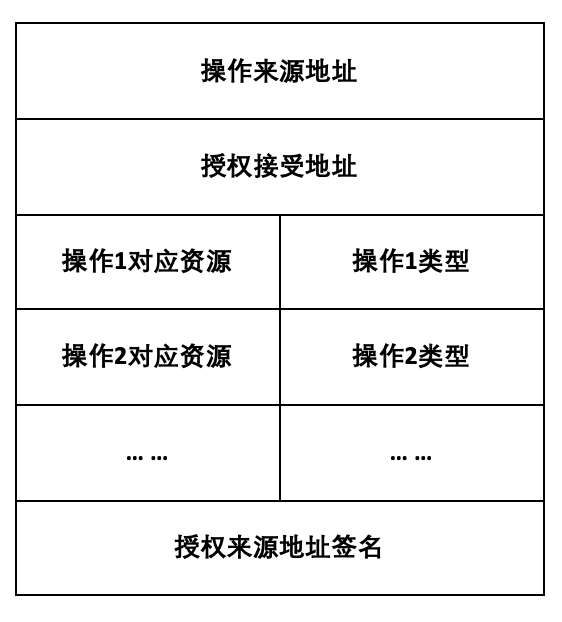
\includegraphics[width=6cm]{figures/op-data.pdf}}
  \caption{授权信息与访问信息数据结构}
  \label{fig:data-structure}
\end{figure}

\subsection{授权信息隐私保护}

对于授权数据,主要保护授权来源、授权对象和授权属性列表。首先设计统一的授权处理算法,该算法包含所有授权前后的状态的转换以及验证的操作。具体细节在算法\ref{alg:authVerify}中进行介绍。

 \begin{algorithm}
 \floatname{algorithm}{Algorithm}
 \caption{授权验证}\label{alg:authVerify}
   \begin{algorithmic}[!htbp]
   \renewcommand{\algorithmicrequire}{\textbf{Input:}}
   \renewcommand{\algorithmicensure}{\textbf{Output:}}
   \REQUIRE $Authorization$
   \ENSURE  $Verification$
    \STATE $Sender$, $Receiptor$, $Attributes$, $nonce$, $Signature \gets Parse(Authorization)$
    \STATE $AuthorizationHash \gets Hash(Authorizaton)$
    \IF {$CheckSignature(Sender, Hash, Signature) \ne true$}
      \RETURN $false$
    \ENDIF
    \STATE $SenderState \gets GetStateFromAddress(Sender)$
    \IF {$nonce < SenderState.nonce$}
      \RETURN $false$
    \ENDIF
    \FOR {$each Attribute \in Attributes$}
      \IF {$SenderState.VerifyAttribute(Attribute) \ne true$}
        \RETURN $false$
      \ENDIF
    \ENDFOR
    \STATE AddAuthorizationToPool(Authorization)
   \RETURN $true$
   \end{algorithmic}
 \end{algorithm}

利用zk-SNARK技术,可以将该算法转换为同态加密下对多项式的验证,并且利用起始阶段生成的证明密钥和验证密钥,授权用户可以对合法的输入给出可信证明,联盟网络中节点在收到该证明后可以在常数时间复杂度内进行验证,并对状态进行修改。

\subsection{操作信息隐私保护}

对于操作数据,与授权数据的不同之处在于,资源服务器必须针对资源进行正确的操作,因此必须知晓操作对象和操作类型,而需要保护操作来源。算法\ref{alg:authVerify}介绍了对操作进行验证的具体步骤。

 \begin{algorithm}
 \floatname{algorithm}{Algorithm}
 \caption{验证操作}
   \begin{algorithmic}[H]\label{alg:opVerify}
   \renewcommand{\algorithmicrequire}{\textbf{Input:}}
   \renewcommand{\algorithmicensure}{\textbf{Output:}}
   \REQUIRE $Operation$
   \ENSURE  $Verification$
    \STATE $Sender$, $OpCode$, $Obj$, $nonce$, $Timestamp$, $Signature \gets Parse(Operation)$
    \STATE $OperationHash \gets Hash(Operation)$
    \IF {$CheckSignature(Sender, Hash, Signature) \ne true$}
      \RETURN $false$
    \ENDIF
    \STATE $SenderState \gets GetStateFromAddress(Sender)$
    \IF {$nonce < SenderState.nonce$}
      \RETURN $false$
    \ENDIF
    \STATE$SubAttributes \gets GetAttrFromAddress(Sender)$
    \STATE$ObjAttributes \gets GetAttrFromObject(Obj)$
    \STATE$OpAttributes \gets GetAttrFromOpCode(OpCode)$
    \STATE$EnvAttributes \gets Timestamp$
    \FOR {$each Policy \in Policies do$}
      \IF {$Policy.Match$($SubAttributes$, $ObjAttributes$, $OpAttributes$, $EnvAttributes$) = $true$}
        \RETURN $true$
      \ENDIF
    \ENDFOR
   \RETURN $false$
   \end{algorithmic}
 \end{algorithm}

在这一算法中,输入的Sender,nonce,Timestamp和Signature信息为隐藏字段,构造在节\ref{sec:zk-SNARK}介绍的$s$中,而OpCode和Obj字段为公开字段,资源服务器根据存储的属性访问控制列表对操作进行验证后得出结论。


% !TeX root = ../main.tex

\chapter{原型实现}
\label{chap:implementation}

\section{系统框架}

\begin{figure}
\centering
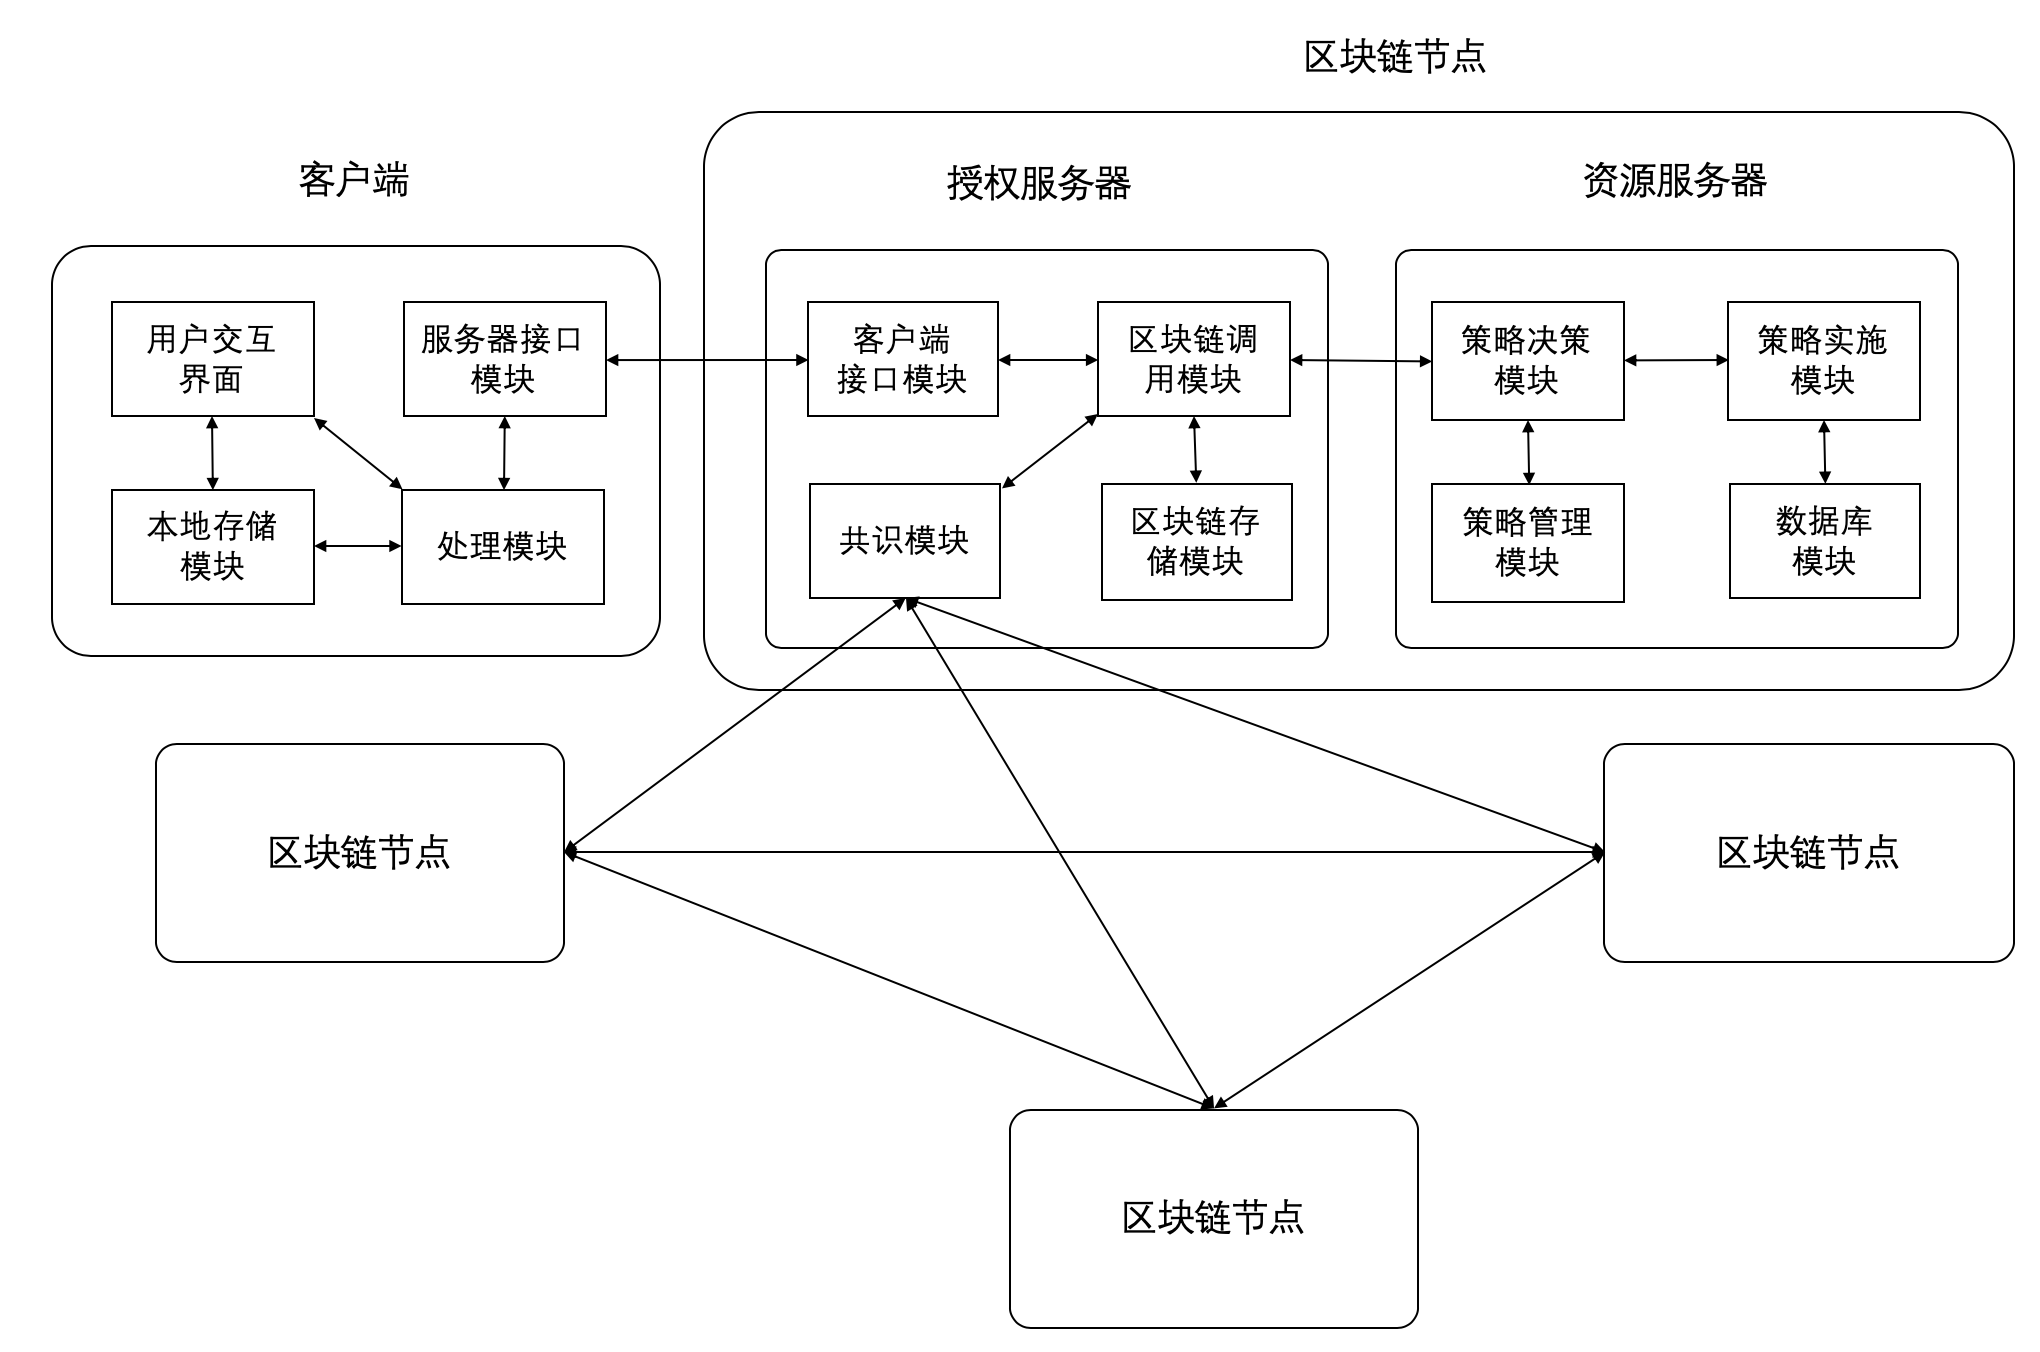
\includegraphics[width=15cm, keepaspectratio]{figures/implementation.pdf}
\caption{系统实现框架图}
\label{fig:implementation}
\end{figure}

如图\ref{fig:implementation}所示,基于上述协议,我们实现了一个原型系统用于验证设计框架和协议的可行性,并且评估性能和延迟等重要指标。

这一系统采用Go程序语言实现,因为Go语言的并发机制(goroutines和channel通信)帮助构建高性能的网络应用,能提升访问控制系统的性能。为了简化实现,客户端、授权服务器以及资源服务器均采用键值对数据库leveldb存储资源,实际上可以采用现有的各类数据库实现。在区块链网络中,节点间的通信采用HTTP协议实现,未来还可以考虑采用UDP协议提升性能。

\begin{description}
  \item \textbf{客户端}:与框架中“客户端”角色不同,这里实现的客户端用于用户管理自己的账户和密钥,授权其他用户,以及操作可访问的资源。该客户端可以生成并签名授权请求和操作请求,并且和服务器节点进行交互。主要实现以下三个模块:
    \begin{enumerate}
      \item 用户交互界面:用户直接查看和操作的界面,用户可以用来完成账号管理、资源访问、授权等操作。
      \item 本地存储模块:在本地存储用户公私钥对、缓存账号属性等信息。
      \item 处理模块:客户端核心模块,负责数据处理,哈希计算,签名及验证等操作。
      \item 服务器接口模块:与服务器进行通信的模块,封装客户端授权,操作数据发送给服务器,以及解析从服务器收到的回应交给处理模块。
    \end{enumerate}
  \item \textbf{授权服务器}:授权服务器主要实现以下四个模块功能:
    \begin{enumerate}
      \item 客户端接口模块:该模块接受客户端的授权请求和操作请求并转发给核心处理模块,以及将处理结果返回给客户端。
      \item 区块链存储模块:该模块根据核心处理模块的指令,负责区块数据以及状态数据的存储和更新。
      \item 共识模块:该模块发送并接受改进的PBFT协议中的相关消息,包括预准备信息,准备信息,承诺信息,更新视图等。采用多个定时器通过管道实现,保障在限定时间内达成共识产生新区块。
      \item 核心处理模块:该模块处理从客户端或者其他节点接收到的消息,运行前文介绍的区块生成和验证算法。
    \end{enumerate}
  \item \textbf{资源服务器}:资源服务器主要由以下四个模块组成:
    \begin{enumerate}
      \item 策略实施模块:接受用户的操作请求,访问授权服务器中区块链模块获取相应的属性信息,将带属性的操作请求发送给策略决策模块。然后根据返回的决策,决定对数据库模块进行相应操作或者拒绝请求。
      \item 策略决策模块:在接收到来自策略实施模块的带属性的操作请求后,向策略管理模块请求相关的访问控制策略,并根据返回的策略对操作请求进行验证。
      \item 策略管理模块:该模块保存基于属性的访问控制列表,根据策略决策模块的请求返回相应的访问控制策略。
      \item 数据库模块:该模块管理用户存储资源的数据库,并根据策略实施模块的操作请求对数据进行增加、删除、修改以及查询操作。
    \end{enumerate}
\end{description}

\section{客户端实现}

\begin{figure}[htb]
\centering
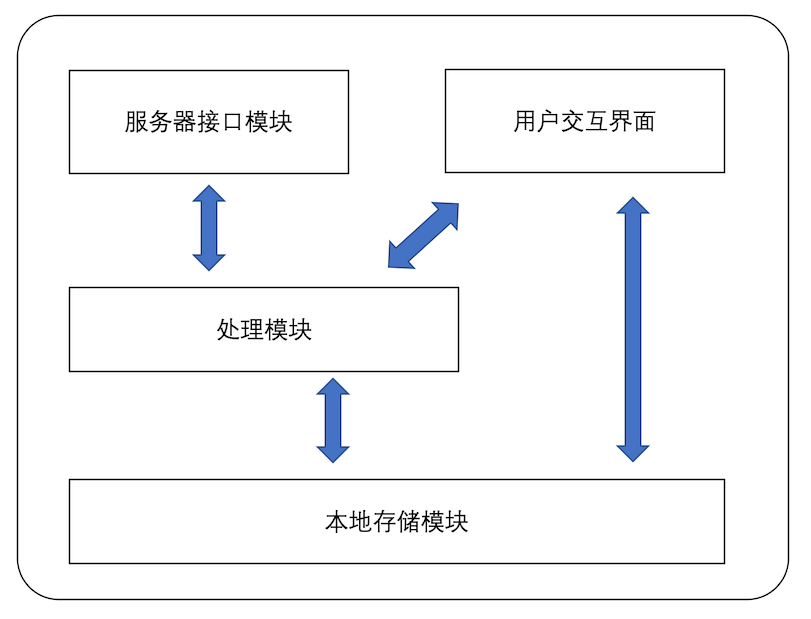
\includegraphics[width=12cm, keepaspectratio]{figures/client.pdf}
\caption{客户端}
\label{fig:client}
\end{figure}

如图\ref{fig:client}所示,客户端主要包含用户交互界面,本地存储模块,处理模块和服务器接口模块三个部分。其中用户交互界面以网页的形式供用户直接查看和操作,主要由前端代码实现。本地存储模块主要实现用户的账号管理,存储账号的公私钥对,属性等信息。服务器接口模块实现与与服务器通信,根据设计的协议封装用户的操作以及解析从服务器收到的回应数据,并通过调用哈希函数,非对称密码库等密码学组件完成签名及验证等操作。

\subsection{用户交互界面}

\begin{figure}[H]
\centering
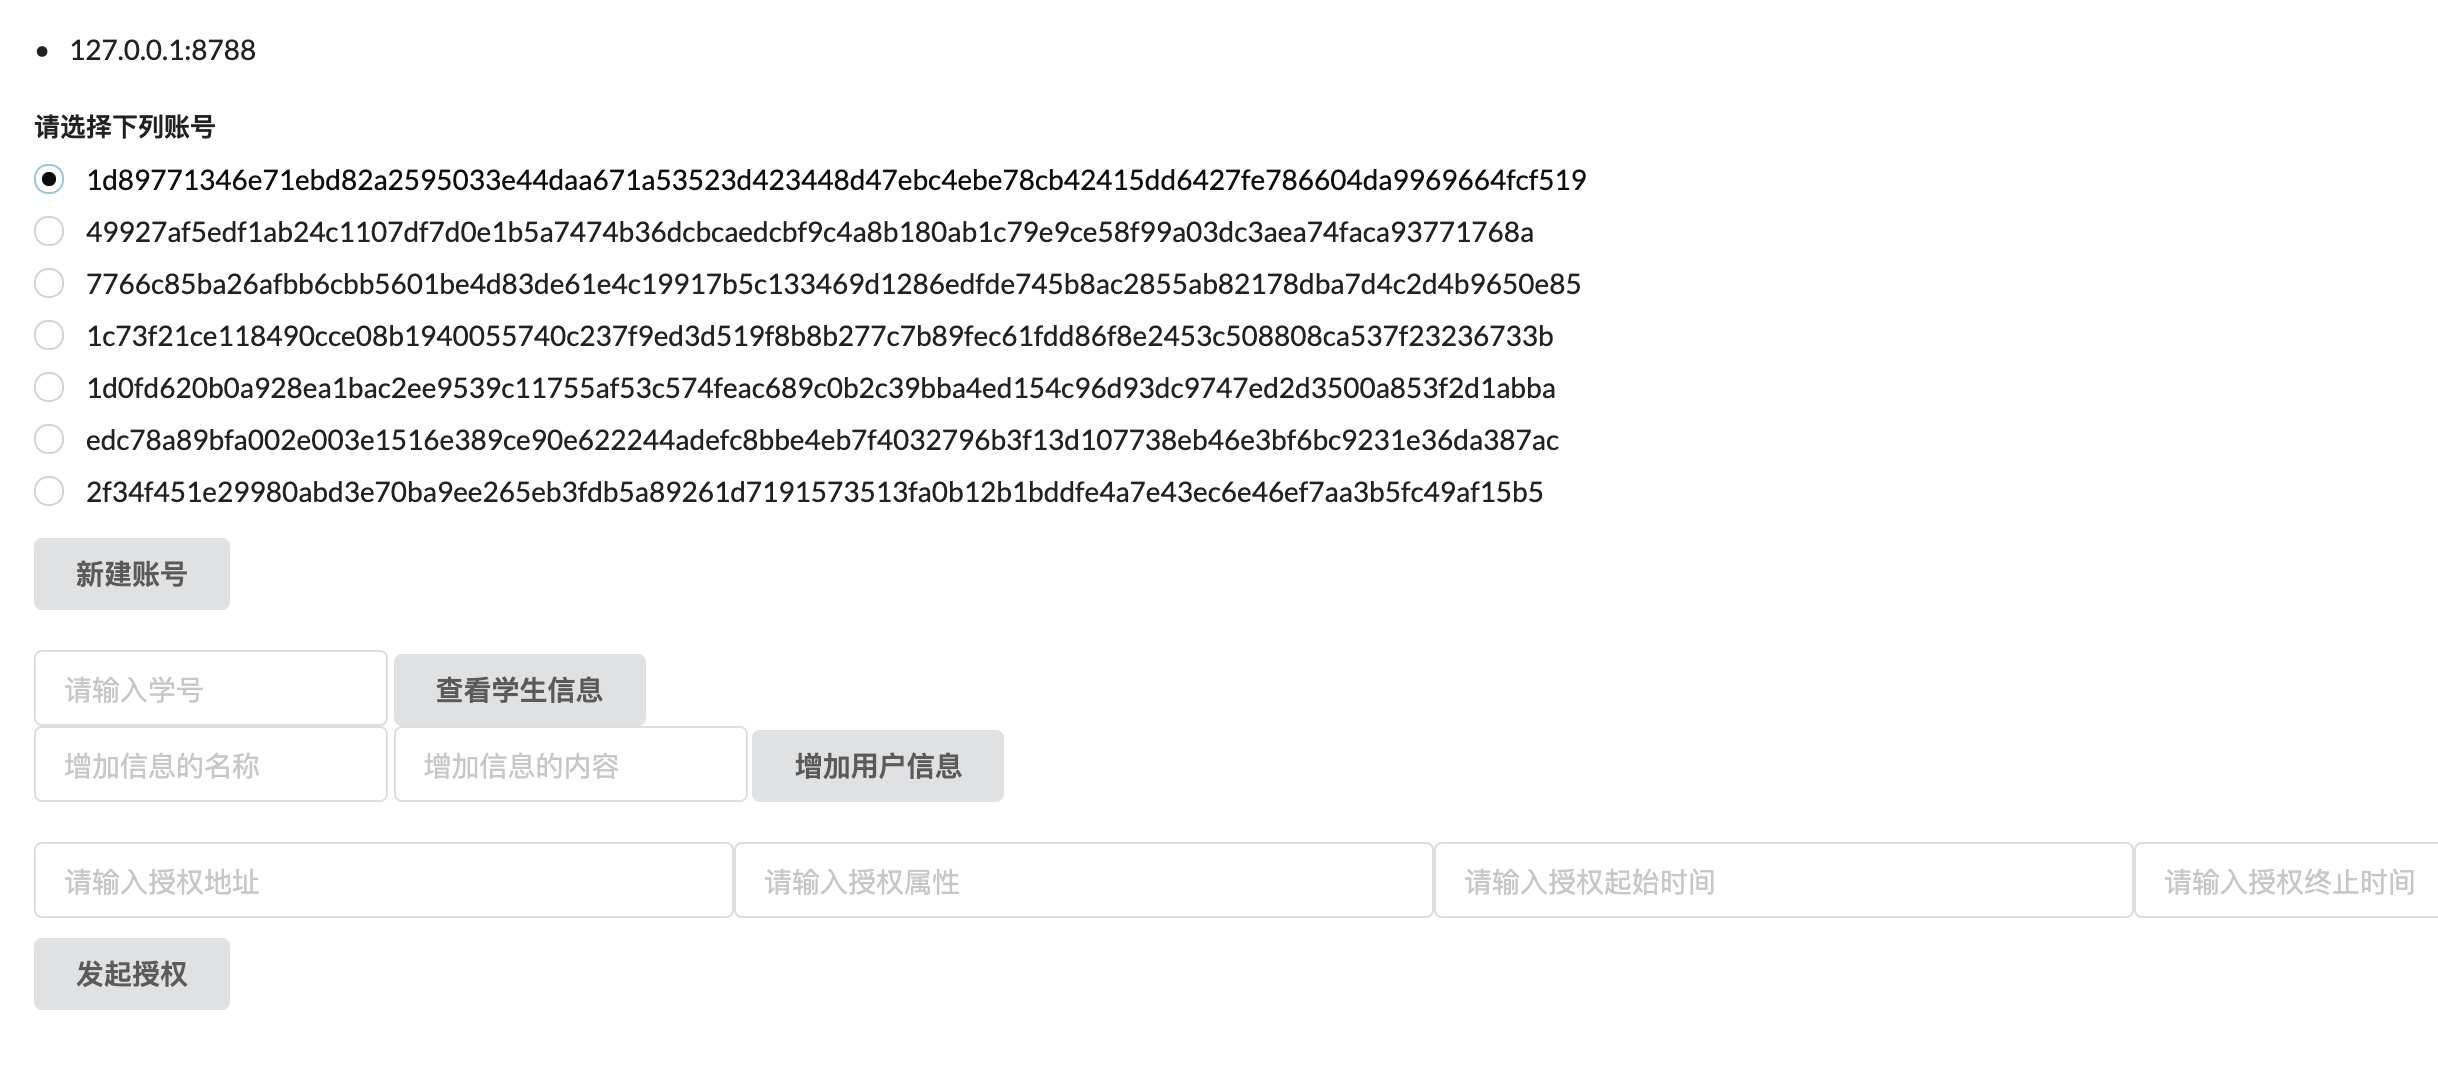
\includegraphics[width=12cm, keepaspectratio]{figures/ui.png}
\caption{用户交互界面}
\label{fig:ui}
\end{figure}

如图\ref{fig:ui}所示,用户交互界面以网页的形式供用户直接查看和操作,用户可以通过“新建账号”按钮创建账号,并选择当前本地已有的任意账号。选定账号后,用户可以通过查看信息,增加信息,修改信息,删除信息等接口对资源进行操作。并且可以通过授权接口,将自己的属性在选定的时间内授权给其他账号。交互界面中,html代码实现界面各元素,css代码实现各文本框及按钮等元素的样式,js代码实现各按钮的交互功能,以及和处理模块进行数据交互。

\subsection{处理模块}

处理模块负责客户端的数据处理,一方面接受来自用户交互界面的账户操作,根据请求数据对本地存储模块进行更新。另一方面,处理用户发起的授权操作和资源操作请求,将请求数据转发到服务器接口模块,由该模块解析并重新封装后发送给服务器。数据处理的过程中调用哈希函数,椭圆曲线等密码学库完成哈希计算,消息签名及签名验证等操作。

\subsection{本地存储模块}

本地存储模块存储用户公私钥对信息,当处理模块需要时提供用于签名或验证。现有各类区块链钱包管理系统用于安全管理账户信息,为了实现简单,本系统以json格式的文件对账户信息进行存储。

\subsection{服务器接口模块}

服务器接口模块负责与服务器进行通信。封装客户端授权数据和操作数据发送给服务器,以及解析从服务器收到的回应转发给处理模块。

\section{授权服务器实现}

\begin{figure}[H]
\centering
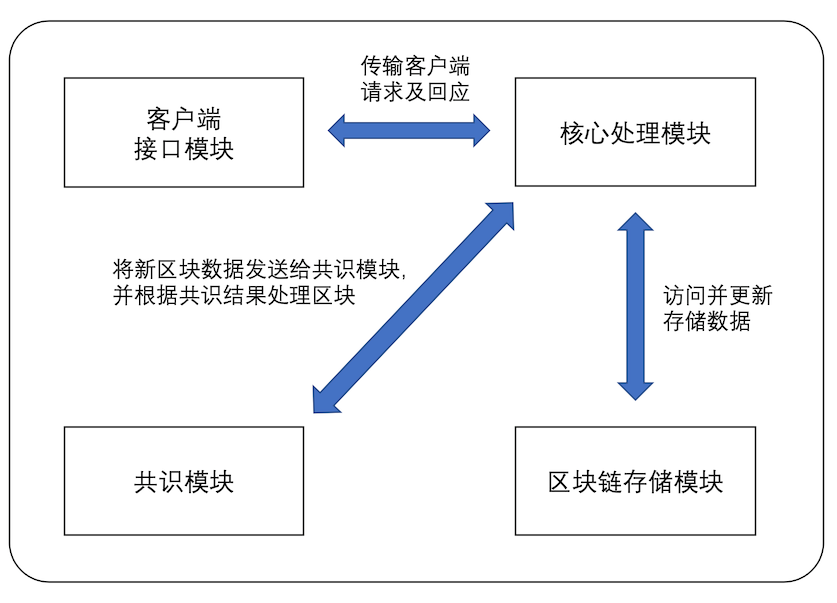
\includegraphics[width=12cm, keepaspectratio]{figures/imple-auth.pdf}
\caption{授权服务器实现框架}
\label{fig:imple-auth}
\end{figure}

授权服务器主要实现客户端接口模块,区块链调用模块,区块链存储模块以及共识模块四个模块功能。其中客户端接口模块负责接受客户端的授权请求和操作请求并转发给核心处理模块,以及将处理结果返回给客户端。区块链存储模块根据核心处理模块的指令,负责区块数据以及状态数据的存储和更新。共识模块与其他区块链节点相连,发送并接收共识协议中的相关消息,包括预准备信息,准备信息,承诺信息,更新视图等。采用多个定时器通过管道实现,保障在限定时间内达成共识产生新区块。核心处理模块负责处理从客户端或者其他区块链节点接收到的数据,运行第\ref{chap:bacs}介绍的授权验证、区块生成等算法。

\subsection{客户端接口模块}

该模块接受客户端的授权请求和操作请求并转发给处理器模块,以及将处理结果返回给客户端。根据预先定义的授权和操作数据结构,负责数据的解析和封装。

\subsection{核心处理模块}

该模块处理从客户端或者其他节点接收到的消息,将通过验证的授权数据存放在授权池,根据共识模块的信号从授权池中选取授权打包成新区块,提交给共识模块。

\subsection{区块链存储模块}

该模块负责存储区块链数据,采用leveldb数据库对区块链链上数据进行存储。该模块在每次核心处理模块启动时,需要提供达成共识的区块链历史数据。在共识模块达成共识后,由核心处理模块将新区块数据发送给存储模块写入数据库。

\subsection{共识模块}

\begin{figure}
\centering
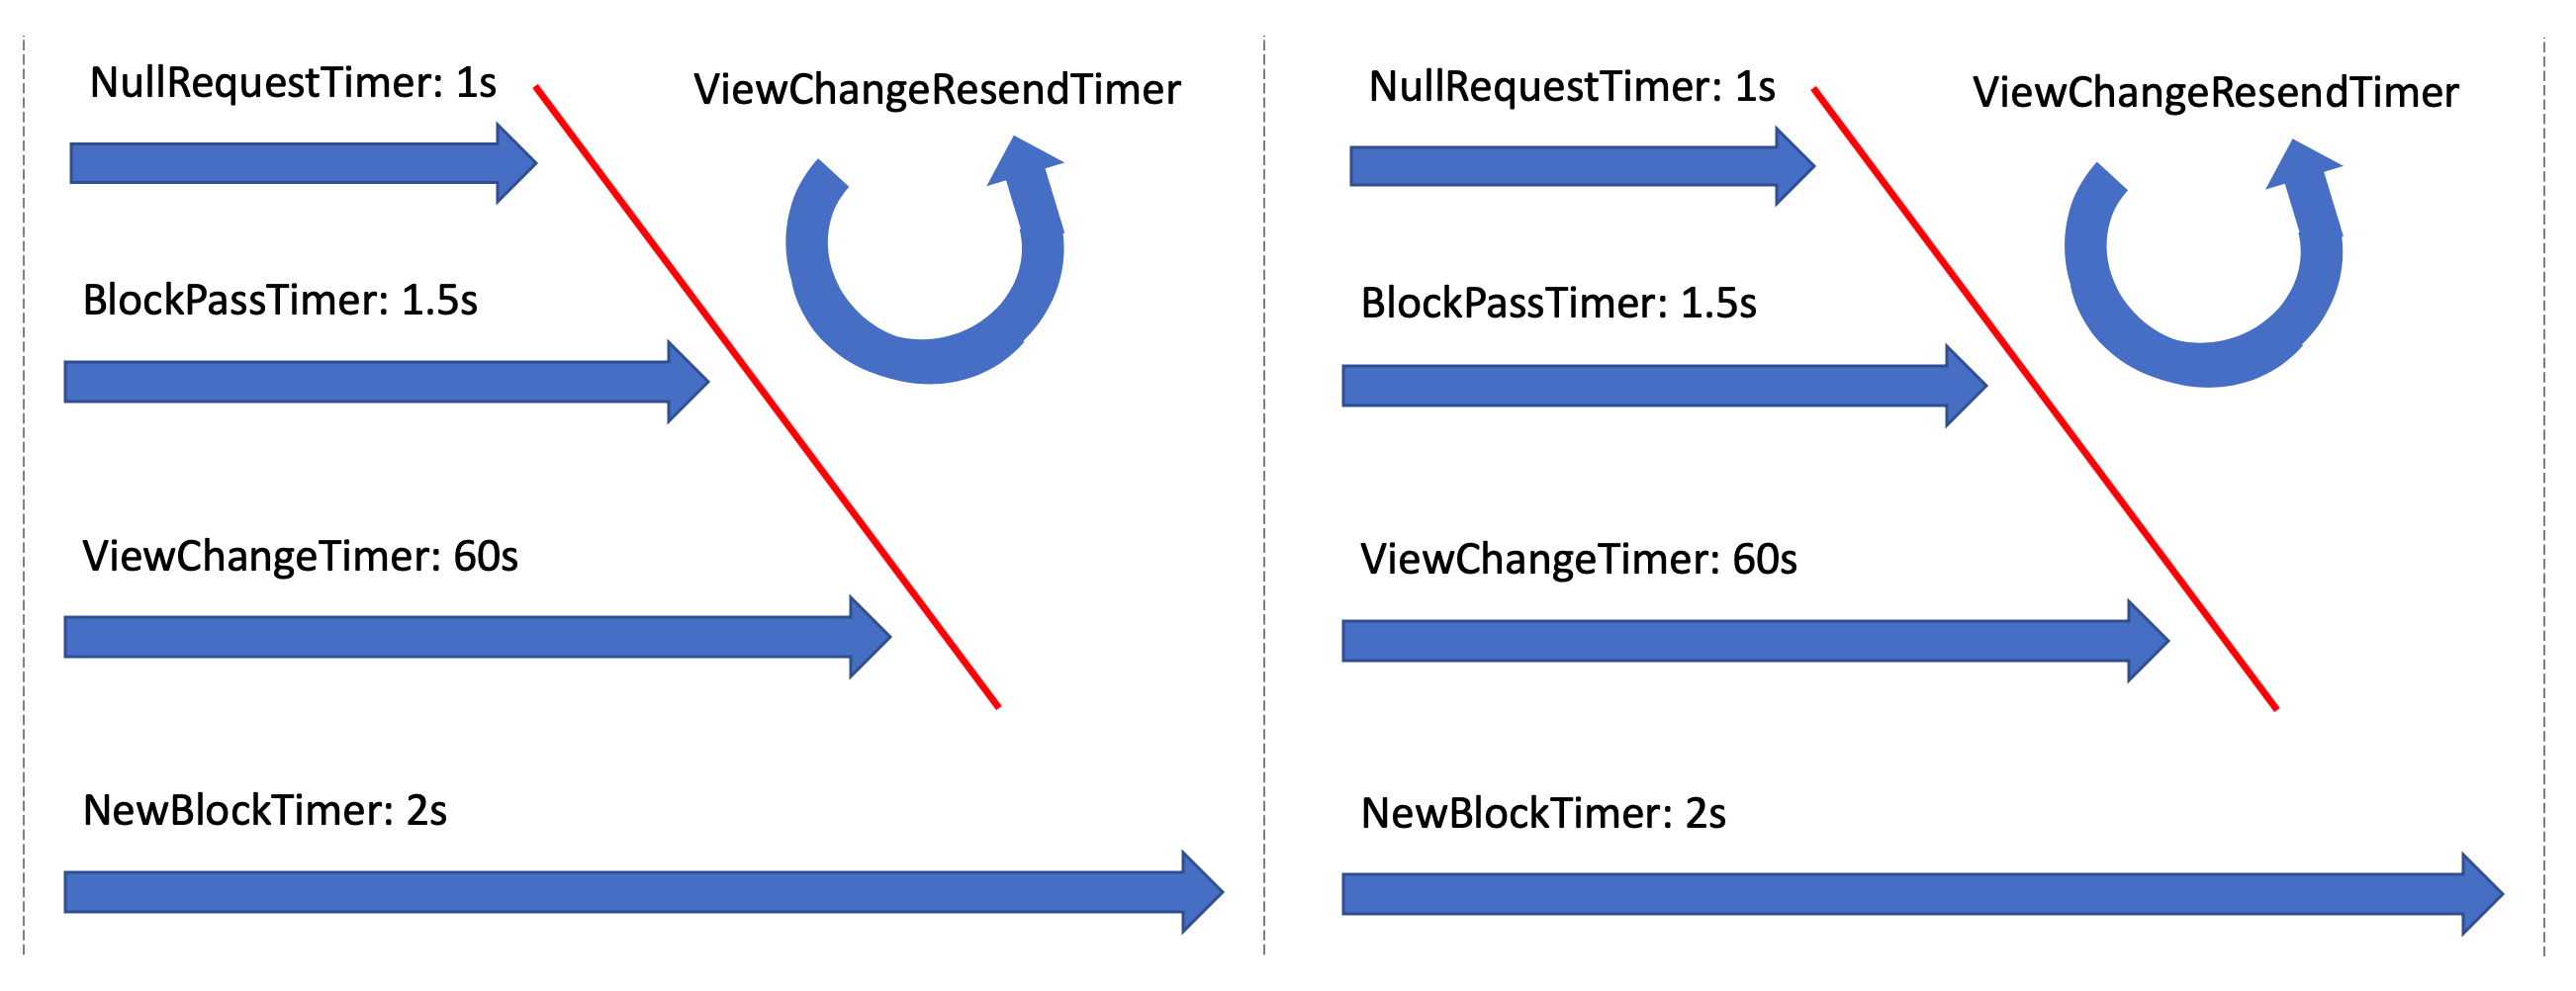
\includegraphics[width=15cm, keepaspectratio]{figures/timer.pdf}
\caption{定时器工作流程}
\label{fig:timer}
\end{figure}

共识模块采用第\ref{subsec:adapted-pbft}节中介绍的共识协议,主要通过若干定时器启动函数,保障协议的正常进行。如图\ref{fig:timer},该系统中,正常情况下由NewBlockTimer每2秒启动一次NewBlock函数,开始一轮新的共识。当每轮共识开始时,启动NullRequestTimer和BlockPassTimer,如果节点在1秒内没有接收到来自主节点的消息,则NullRequestTimer到期。如果节点在1.5秒内没有收到足够多的“承诺消息”表示共识达成,则BlockPassTimer到期。为了保障在一定时间后主节点切换,ViewChangeTimer设置为每60秒到期一次,无法中断。这三个定时器到期,节点都会发起视图切换,开始不断循环ViewChangeResendTimer尝试切换到下一个视图,直到与其他节点达成共识成功切换视图为止。

\section{资源服务器实现}

\begin{figure}[ht]
\centering
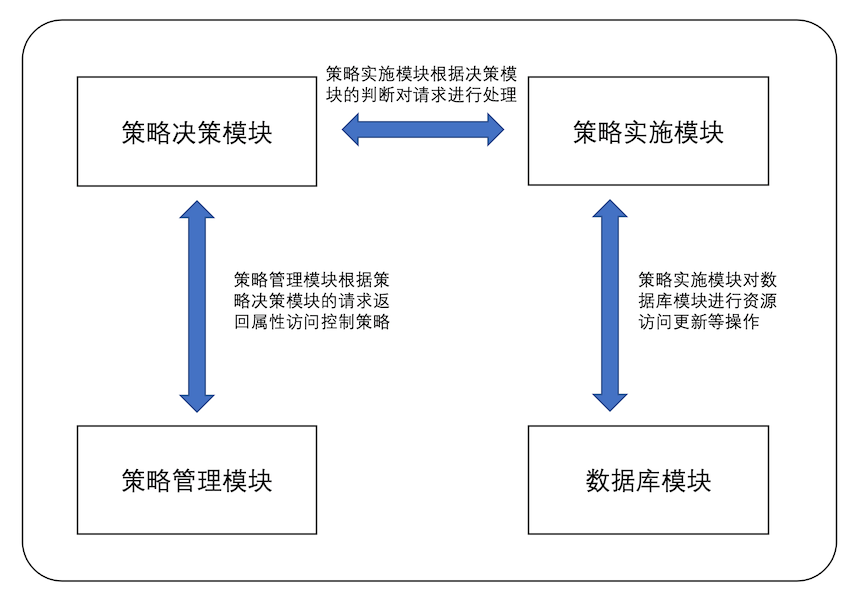
\includegraphics[width=12cm, keepaspectratio]{figures/imple-resource.pdf}
\caption{资源服务器实现框架}
\label{fig:imple-resource}
\end{figure}

如图\ref{fig:imple-resource}所示,资源服务器主要由以下四个模块组成,数据库模块管理用户存储资源的数据库,并根据访问控制模块的验证结果对数据进行操作。策略管理模块保存基于属性的访问控制列表。策略决策模块对访问请求进行决策。策略实施模块根据策略决策模块的判断对数据库模块进行操作,并回应请求。

\subsection{策略实施模块}

策略实施模块接收来自用户的操作请求,如果消息与签名不符合则直接拒绝该请求。在验证签名后,策略实施模块根据当前时间补充上时间戳字段作为环境属性,提交给策略决策模块。等待策略决策模块回应决策结果后,策略实施模块将操作请求中具体操作的信息发送给数据库模块。最后将数据库模块返回的操作结果发送给请求用户。

\subsection{策略决策模块}

策略决策模块接收来自策略实施模块的带属性的操作请求,解析出其中主体属性、客体属性、操作属性以及环境属性,根据各属性从策略管理模块中获取相关的访问控制策略。控制策略列表中的各策略包含主体属性、客体属性、操作属性以及环境属性四个部分,其中主体属性、客体属性以及操作属性由逻辑表达式构成,当操作请求中的各项属性满足逻辑表达式即满足。环境属性只包含时间戳,由起始时间和终止时间两个字段组成,当操作请求中的时间戳在起始时间和终止时间组成的区间内即满足。如果操作请求满足访问控制策略列表中任何一项策略,则通过验证。策略决策模块将验证后的结果返回给策略实施模块。

\subsection{策略管理模块}

本原型系统不考虑策略列表的初始化和更新,策略管理模块只负责存储访问控制策略列表,当接受到策略决策模块关于带有某些属性的访问策略请求时,返回对应策略。为了简化实现,访问控制列表以json形式文件存储。

\subsection{数据库模块}

该原型实现中,数据库模块采用LevelDB键值数据库存放管理用户信息,每个用户拥有唯一编号。可以根据该编号查询用户信息,以及对信息进行增加、删除、修改等操作。操作请求的数据结构主要包含用户编号、操作类型、操作字段、操作值四个数据。其中当操作类型为查询时,操作字段和操作值可以为空。当操作类型为删除时,操作值可以为空。当操作类型为新增和修改时,所有字段都不能为空。

\section{性能测试}

\begin{figure}[H]
\centering
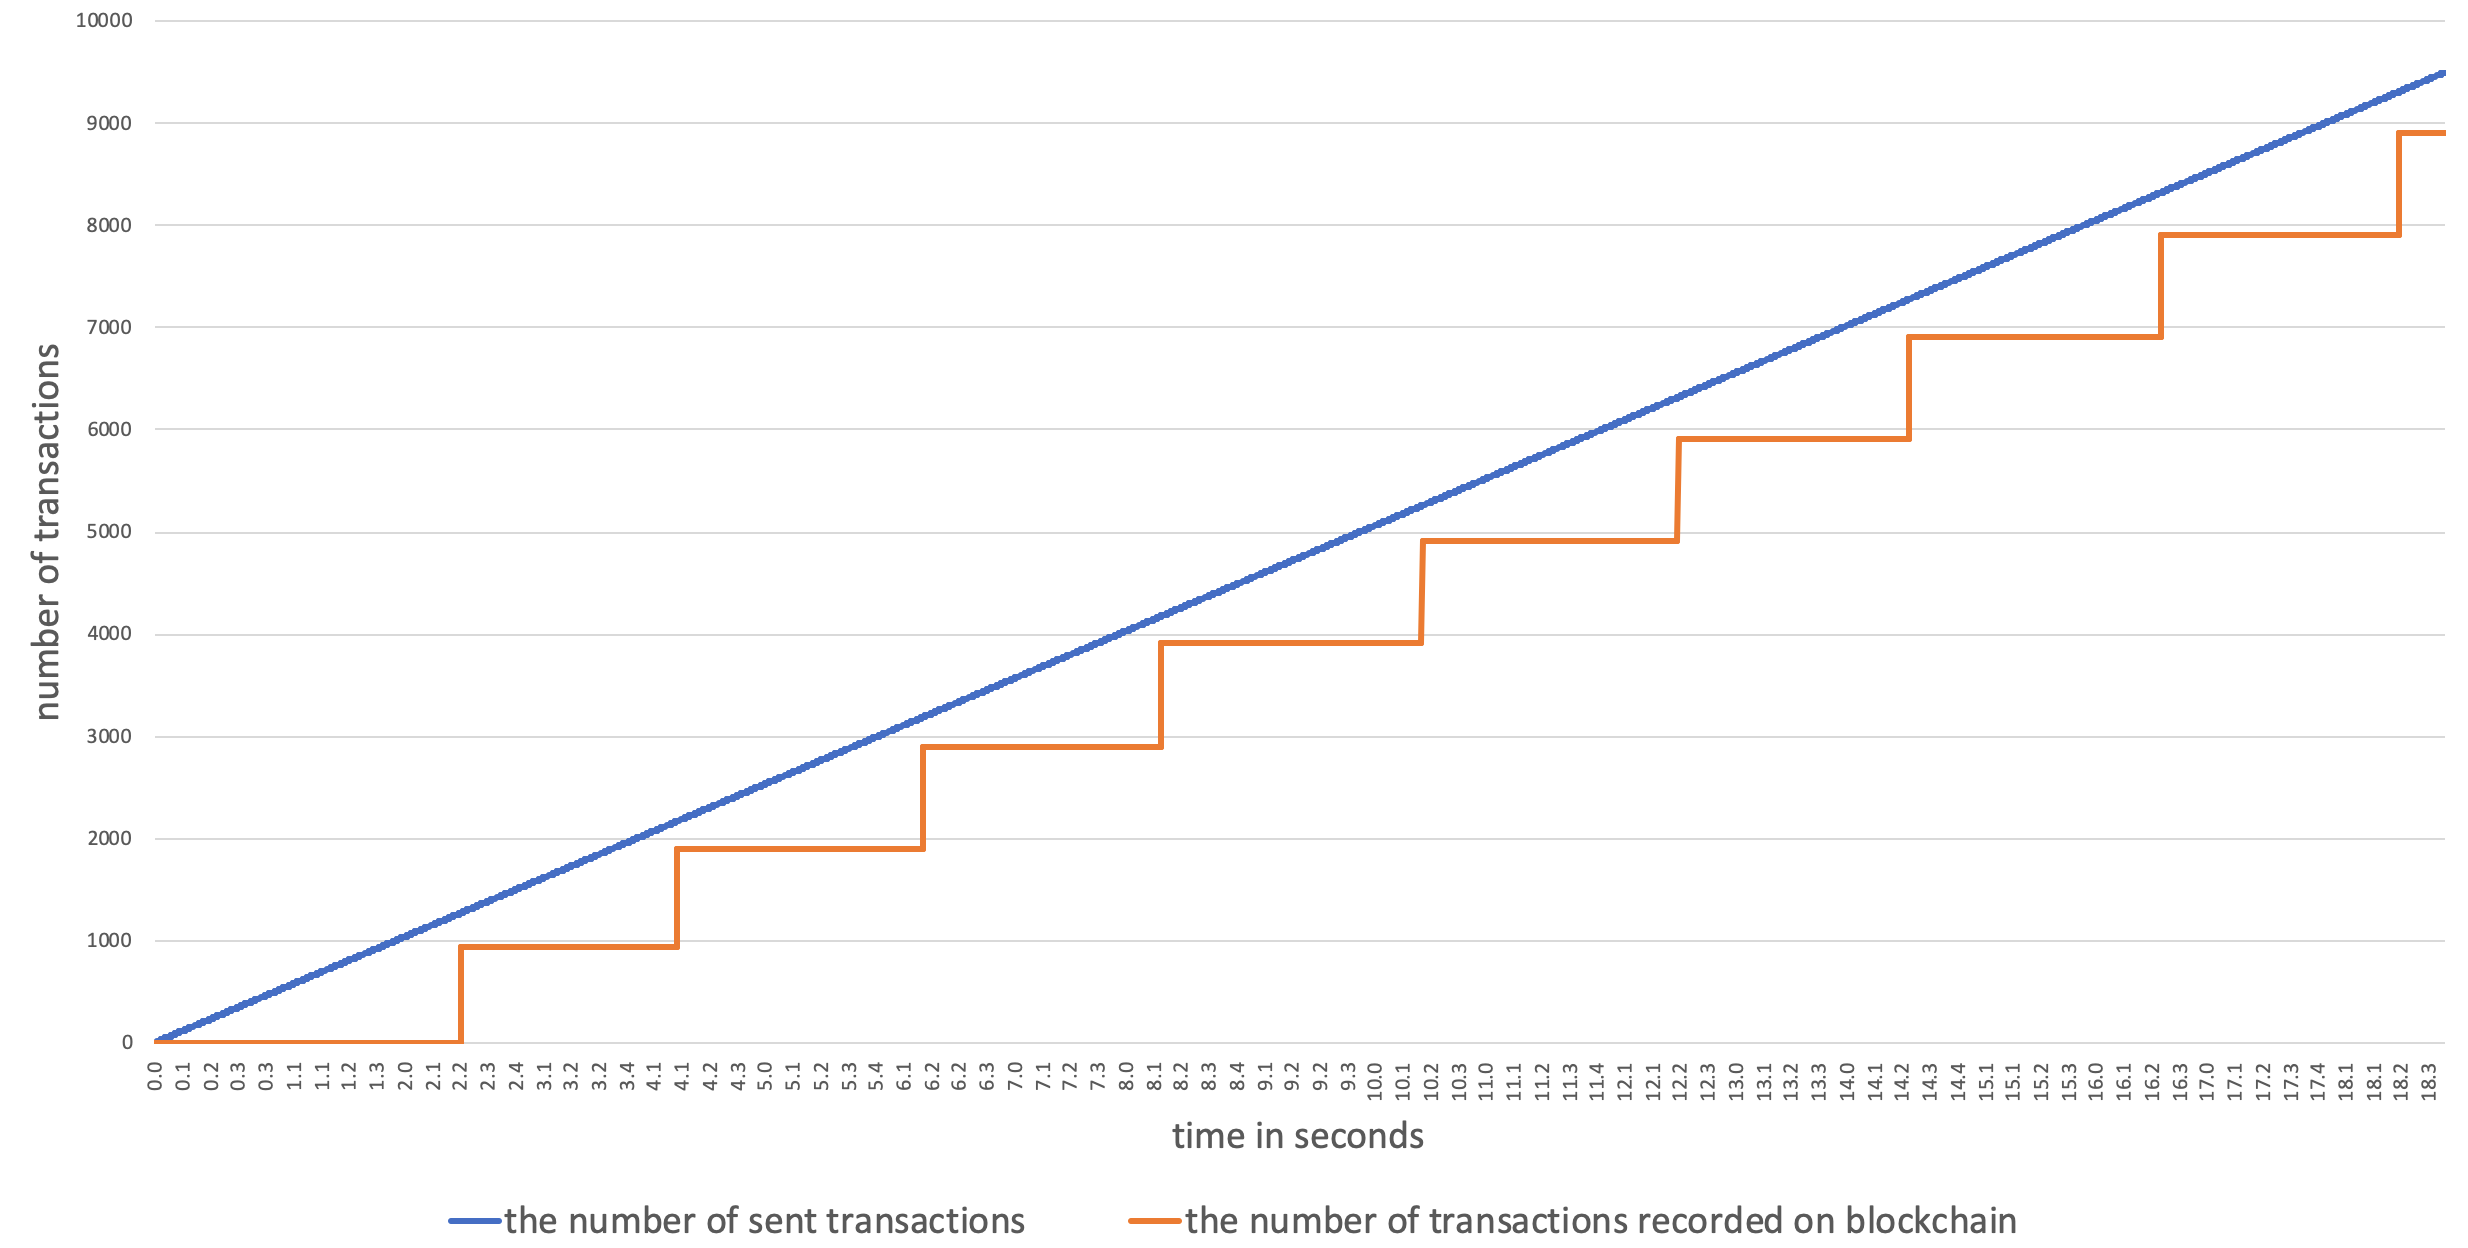
\includegraphics[width=12cm, keepaspectratio]{figures/performance.png}
\caption{性能测试}
\label{fig:performance}
\end{figure}

我们在微软云平台上部署了四个区块链节点,每个节点采用标准的D2s v3型号服务器,拥有2 vCPU,2G内存以及1000 MBps网络带宽。为了测试系统性能,我们生成了1000对公私钥对来模拟1000个用户,每个用户拥有不同的属性,还在随机用户之间生成了10000个随机的授权操作,用于模拟现实中的授权行为。

测试授权数据以每秒500个授权的速率发送给4个节点,区块链网络在大概21秒的时间里成功处理了这些请求。发送的分布时间如图\ref{fig:performance}所示。该网络每2秒生成一个新区块,并且每个区块最多包含1000个授权请求(这一限制设置在代码中)。每个区块包含的授权信息数量如图\ref{fig:performance}所示。实验证明了该系统可以达到每秒处理500个授权请求并且平均延迟在1秒左右,这说明该框架和协议可以应用于部分现实场景中。并且在性能上还可以通过增加服务器性能、带宽,优化通信协议等方式提升。
% !TeX root = ../main.tex

\chapter{总结与展望}

\section{全文总结}

访问控制领域是计算机系统中重要的研究领域,直接关系数据的安全和隐私。访问控制模型的发展已经较为成熟,DAC、MAC、RBAC、ABAC等访问控制模型被普遍应用。随着互联网应用的发展,为了提升访问控制的灵活性,OAuth 2.0框架广泛用于互联网中向第三方应用提供授权服务。OAuth及类似框架都存在严重中心化的授权服务器,成为系统的性能瓶颈和安全隐患。

区块链技术能保障存储数据的安全性,但由于性能和存储有限,难以在各领域实际应用。访问控制领域的授权数据刚好满足这两点特性,一方面授权数据需要较高的安全性保障,另一方面,授权数据相较于业务数据而言规模较小。基于这些特点,本文提出基于区块链技术的授权服务系统B-OAuth,主要进行以下技术的改进和创新:

\begin{enumerate}
	\item 针对授权服务框架中存在的中心化授权服务器,提出了区块链网络替代方案,增强系统的安全性和鲁棒性。
	\item 针对区块链账本的存储模式,对基于属性的访问控制系统进行改进,定义符合区块链特点的授权数据结构。
	\item 针对区块链网络存在的用户隐私泄漏风险,引入zk-snark技术,提出了对授权和操作进行隐私保护的方法。
\end{enumerate}

\section{未来展望}

基于区块链的访问控制系统未来有广泛的应用场景,但相关研究还较少。本文提出了一些技术的改进,但仍在框架设计、技术细节等方面存在一些需要改进的空间,后续的研究可以从以下几个方面进行:

\begin{enumerate}
	\item 本文只提出了基于属性的访问控制模型和区块链技术的结合,还可以研究现有其他各访问控制模型基于区块链的实现,增强该系统对现有访问控制系统的兼容性。
	\item 本文采用了改进的PBFT共识协议,该共识协议在性能、扩展性方面还存在不足,难以应用于多节点网络,因此还可以研究性能更高的共识协议。
	\item 本文只是提出了对授权和操作进行隐私保护的设计和功能实现方案,还未将该方法结合现有系统进行完整的实现,后续可以将整个系统的存储数据结构进行修改,满足隐私保护特性。
\end{enumerate}


% 其它部分
% \backmatter

%% 本科生要求的几个索引。
% \listoffigures    % 插图索引
% \listoftables     % 表格索引
% \listofequations  % 公式索引

% 参考文献
\bibliographystyle{thuthesis-numeric}      % 顺序编码制
\bibliographystyle{thuthesis-author-year}  % 著者-出版年制
\bibliographystyle{thuthesis-bachelor}     % 本科生参考文献的著录格式
\bibliography{ref/refs}

% 致谢
% \input{data/acknowledgements}

% 声明
% \statement

% 附录
% \appendix
% \input{data/appendix-survey}       % 本科生:外文资料的调研阅读报告
% \input{data/appendix-translation}  % 本科生:外文资料的书面翻译
% \input{data/appendix}

% 个人简历
% % !TeX root = ../main.tex

\begin{resume}

  \resumeitem{个人简历}

  1995 年 07 月 25 日出生于 四川 省 资阳 市。

  2013 年 9 月考入 北京航空航天 大学 计算机科学与技术 系 计算机科学与技术 专业,2017 年 7 月本科毕业并获得 工学 学士学位。

  2017 年 9 月 研究生统一招生考试 进入 清华 大学 计算机科学与技术 系攻读 硕士 学位至今。

  \researchitem{发表的学术论文} % 发表的和录用的合在一起

  % 1. 已经刊载的学术论文(本人是第一作者,或者导师为第一作者本人是第二作者)
  \begin{publications}
    \item Zhang A., Bai X. (2020) Decentralized Authorization and Authentication Based on Consortium Blockchain. In: Zheng Z., Dai HN., Tang M., Chen X. (eds) Blockchain and Trustworthy Systems. BlockSys 2019. Communications in Computer and Information Science, vol 1156. Springer, Singapore (EI 收录, 检索号:20200708163648.)
  \end{publications}

  % 2. 尚未刊载,但已经接到正式录用函的学术论文(本人为第一作者,或者
  %    导师为第一作者本人是第二作者)。
  \begin{publications}[before=\publicationskip,after=\publicationskip]
    \item 张 奥, 白晓颖. 区块链隐私保护研究与实践综述 (已被 软件学报 录用. TH-CPL B类期刊.)
  \end{publications}

  % 3. 其他学术论文。可列出除上述两种情况以外的其他学术论文,但必须是
  %    已经刊载或者收到正式录用函的论文。
  % \begin{publications}
  %   \item Wu X M, Yang Y, Cai J, et al. Measurements of ferroelectric MEMS
  %     microphones. Integrated Ferroelectrics, 2005, 69:417-429. (SCI 收录, 检索号
  %     :896KM)
  %   \item 贾泽, 杨轶, 陈兢, 等. 用于压电和电容微麦克风的体硅腐蚀相关研究. 压电与声
  %     光, 2006, 28(1):117-119. (EI 收录, 检索号:06129773469)
  %   \item 伍晓明, 杨轶, 张宁欣, 等. 基于MEMS技术的集成铁电硅微麦克风. 中国集成电路,
  %     2003, 53:59-61.
  % \end{publications}

  % \researchitem{研究成果} % 有就写,没有就删除
  % \begin{achievements}
  %   \item 任天令, 杨轶, 朱一平, 等. 硅基铁电微声学传感器畴极化区域控制和电极连接的
  %     方法: 中国, CN1602118A. (中国专利公开号)
  %   \item Ren T L, Yang Y, Zhu Y P, et al. Piezoelectric micro acoustic sensor
  %     based on ferroelectric materials: USA, No.11/215, 102. (美国发明专利申请号)
  % \end{achievements}

\end{resume}


% 本科生的综合论文训练记录表
% \includepdf[pages=-]{scan-record.pdf}

\end{document}
